\documentclass[ignorenonframetext,]{beamer}
\setbeamertemplate{caption}[numbered]
\setbeamertemplate{caption label separator}{: }
\setbeamercolor{caption name}{fg=normal text.fg}
\beamertemplatenavigationsymbolsempty
\usepackage{lmodern}
\usepackage{amssymb,amsmath}
\usepackage{ifxetex,ifluatex}
\usepackage{fixltx2e} % provides \textsubscript
\ifnum 0\ifxetex 1\fi\ifluatex 1\fi=0 % if pdftex
  \usepackage[T1]{fontenc}
  \usepackage[utf8]{inputenc}
\else % if luatex or xelatex
  \ifxetex
    \usepackage{mathspec}
  \else
    \usepackage{fontspec}
  \fi
  \defaultfontfeatures{Ligatures=TeX,Scale=MatchLowercase}
\fi
\usetheme{AnnArbor}
\usecolortheme{dolphin}
\usefonttheme{professionalfonts}
% use upquote if available, for straight quotes in verbatim environments
\IfFileExists{upquote.sty}{\usepackage{upquote}}{}
% use microtype if available
\IfFileExists{microtype.sty}{%
\usepackage{microtype}
\UseMicrotypeSet[protrusion]{basicmath} % disable protrusion for tt fonts
}{}
\newif\ifbibliography
\usepackage{color}
\usepackage{fancyvrb}
\newcommand{\VerbBar}{|}
\newcommand{\VERB}{\Verb[commandchars=\\\{\}]}
\DefineVerbatimEnvironment{Highlighting}{Verbatim}{commandchars=\\\{\}}
% Add ',fontsize=\small' for more characters per line
\usepackage{framed}
\definecolor{shadecolor}{RGB}{248,248,248}
\newenvironment{Shaded}{\begin{snugshade}}{\end{snugshade}}
\newcommand{\KeywordTok}[1]{\textcolor[rgb]{0.13,0.29,0.53}{\textbf{{#1}}}}
\newcommand{\DataTypeTok}[1]{\textcolor[rgb]{0.13,0.29,0.53}{{#1}}}
\newcommand{\DecValTok}[1]{\textcolor[rgb]{0.00,0.00,0.81}{{#1}}}
\newcommand{\BaseNTok}[1]{\textcolor[rgb]{0.00,0.00,0.81}{{#1}}}
\newcommand{\FloatTok}[1]{\textcolor[rgb]{0.00,0.00,0.81}{{#1}}}
\newcommand{\ConstantTok}[1]{\textcolor[rgb]{0.00,0.00,0.00}{{#1}}}
\newcommand{\CharTok}[1]{\textcolor[rgb]{0.31,0.60,0.02}{{#1}}}
\newcommand{\SpecialCharTok}[1]{\textcolor[rgb]{0.00,0.00,0.00}{{#1}}}
\newcommand{\StringTok}[1]{\textcolor[rgb]{0.31,0.60,0.02}{{#1}}}
\newcommand{\VerbatimStringTok}[1]{\textcolor[rgb]{0.31,0.60,0.02}{{#1}}}
\newcommand{\SpecialStringTok}[1]{\textcolor[rgb]{0.31,0.60,0.02}{{#1}}}
\newcommand{\ImportTok}[1]{{#1}}
\newcommand{\CommentTok}[1]{\textcolor[rgb]{0.56,0.35,0.01}{\textit{{#1}}}}
\newcommand{\DocumentationTok}[1]{\textcolor[rgb]{0.56,0.35,0.01}{\textbf{\textit{{#1}}}}}
\newcommand{\AnnotationTok}[1]{\textcolor[rgb]{0.56,0.35,0.01}{\textbf{\textit{{#1}}}}}
\newcommand{\CommentVarTok}[1]{\textcolor[rgb]{0.56,0.35,0.01}{\textbf{\textit{{#1}}}}}
\newcommand{\OtherTok}[1]{\textcolor[rgb]{0.56,0.35,0.01}{{#1}}}
\newcommand{\FunctionTok}[1]{\textcolor[rgb]{0.00,0.00,0.00}{{#1}}}
\newcommand{\VariableTok}[1]{\textcolor[rgb]{0.00,0.00,0.00}{{#1}}}
\newcommand{\ControlFlowTok}[1]{\textcolor[rgb]{0.13,0.29,0.53}{\textbf{{#1}}}}
\newcommand{\OperatorTok}[1]{\textcolor[rgb]{0.81,0.36,0.00}{\textbf{{#1}}}}
\newcommand{\BuiltInTok}[1]{{#1}}
\newcommand{\ExtensionTok}[1]{{#1}}
\newcommand{\PreprocessorTok}[1]{\textcolor[rgb]{0.56,0.35,0.01}{\textit{{#1}}}}
\newcommand{\AttributeTok}[1]{\textcolor[rgb]{0.77,0.63,0.00}{{#1}}}
\newcommand{\RegionMarkerTok}[1]{{#1}}
\newcommand{\InformationTok}[1]{\textcolor[rgb]{0.56,0.35,0.01}{\textbf{\textit{{#1}}}}}
\newcommand{\WarningTok}[1]{\textcolor[rgb]{0.56,0.35,0.01}{\textbf{\textit{{#1}}}}}
\newcommand{\AlertTok}[1]{\textcolor[rgb]{0.94,0.16,0.16}{{#1}}}
\newcommand{\ErrorTok}[1]{\textcolor[rgb]{0.64,0.00,0.00}{\textbf{{#1}}}}
\newcommand{\NormalTok}[1]{{#1}}
\usepackage{longtable,booktabs}
\usepackage{caption}
% These lines are needed to make table captions work with longtable:
\makeatletter
\def\fnum@table{\tablename~\thetable}
\makeatother
\usepackage{graphicx,grffile}
\makeatletter
\def\maxwidth{\ifdim\Gin@nat@width>\linewidth\linewidth\else\Gin@nat@width\fi}
\def\maxheight{\ifdim\Gin@nat@height>\textheight0.8\textheight\else\Gin@nat@height\fi}
\makeatother
% Scale images if necessary, so that they will not overflow the page
% margins by default, and it is still possible to overwrite the defaults
% using explicit options in \includegraphics[width, height, ...]{}
\setkeys{Gin}{width=\maxwidth,height=\maxheight,keepaspectratio}

% Prevent slide breaks in the middle of a paragraph:
\widowpenalties 1 10000
\raggedbottom

\AtBeginPart{
  \let\insertpartnumber\relax
  \let\partname\relax
  \frame{\partpage}
}
\AtBeginSection{
  \ifbibliography
  \else
    \let\insertsectionnumber\relax
    \let\sectionname\relax
    \frame{\sectionpage}
  \fi
}
\AtBeginSubsection{
  \let\insertsubsectionnumber\relax
  \let\subsectionname\relax
  \frame{\subsectionpage}
}

\setlength{\emergencystretch}{3em}  % prevent overfull lines
\providecommand{\tightlist}{%
  \setlength{\itemsep}{0pt}\setlength{\parskip}{0pt}}
\setcounter{secnumdepth}{0}


% \pgfdeclareimage[width=1cm]{logo}{./figures/monkeyTypewriter.png}
%\logo{\pgfuseimage{logo}}

\institute{University of Virginia}
\definecolor{links}{RGB}{42, 27, 129}
\definecolor{mypink2}{RGB}{219, 48, 122}
%\hypersetup{colorlinks,linkcolor=links,urlcolor=mypink2}
\usefonttheme{professionalfonts}

% \setbeamerfont{note page}{family*=pplx,size=\footnotesize} % Palatino for notes

\setbeamerfont{subtitle}{size=\small}

\definecolor{uvablue}{RGB}{0,85,150}
\definecolor{uvalibraryorange}{RGB}{252,175,23}
\definecolor{uvacream}{RGB}{241,229,199}
\definecolor{uvalightblue}{RGB}{163,220,230}

\setbeamercolor{block body}{bg=green,fg=green}
\setbeamercolor{block body alerted}{bg=green,fg=green}
\setbeamercolor{block body example}{bg=green,fg=green}

\setbeamercolor{caption name}{fg=uvablue}

\setbeamercolor{headline}{fg=uvacream,bg=uvacream}
\setbeamercolor{section}{fg=uvalibraryorange,bg=uvablue}
\setbeamercolor{frametitle}{fg=uvalibraryorange,bg=uvablue}
\setbeamercolor{palette primary}{bg=uvalibraryorange,fg=uvablue}
\setbeamercolor{palette secondary}{bg=uvablue,fg=uvablue}
\setbeamercolor{palette tertiary}{bg=uvalibraryorange,fg=uvablue}
\setbeamercolor{palette quarternary}{fg=uvalibraryorange,bg=uvablue}
\setbeamercolor{palette sidebar primary}{bg=uvalibraryorange,fg=uvablue}
\setbeamercolor{palette sidebar secondary}{fg=uvablue,bg=uvablue}
\setbeamercolor{palette sidebar tertiary}{fg=uvalibraryorange,bg=uvablue}
\setbeamercolor{palette sidebar quarternary}{fg=uvalibraryorange,bg=uvablue}
\setbeamercolor{structure}{bg=uvablue}



\useinnertheme{rectangles}

\titlegraphic{\vspace{-7.5mm}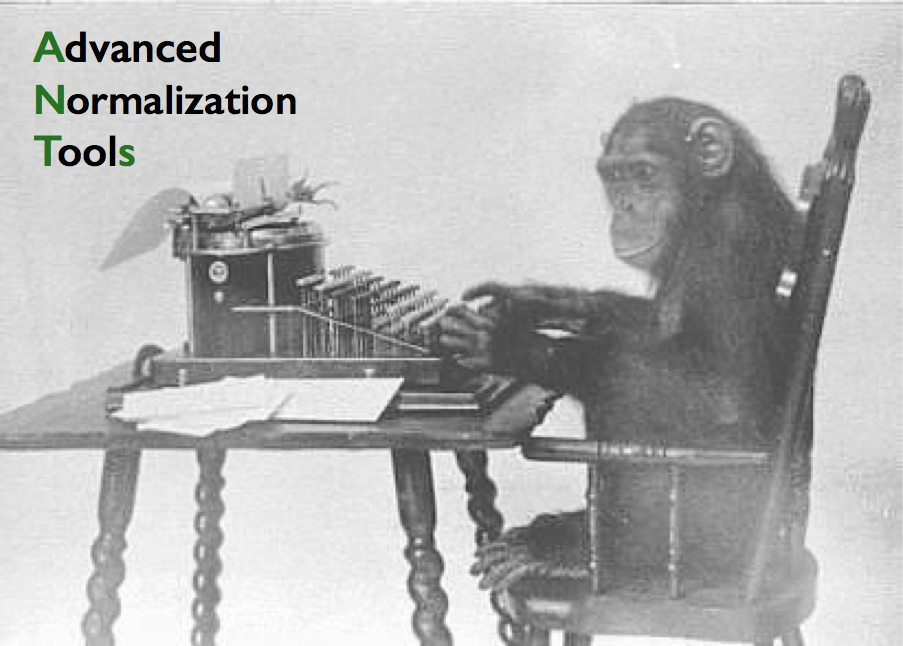
\includegraphics[width=0.45\paperwidth]{./figures/monkeyTypewriter.png}}

\title{``Dr.~Tustison (UVA) presentation''}
\author{Nick Tustison}
\date{}

\begin{document}
\frame{\titlepage}

\section{Developers and
collaborators}\label{developers-and-collaborators}

\begin{frame}{Founders: Brian and Nick}

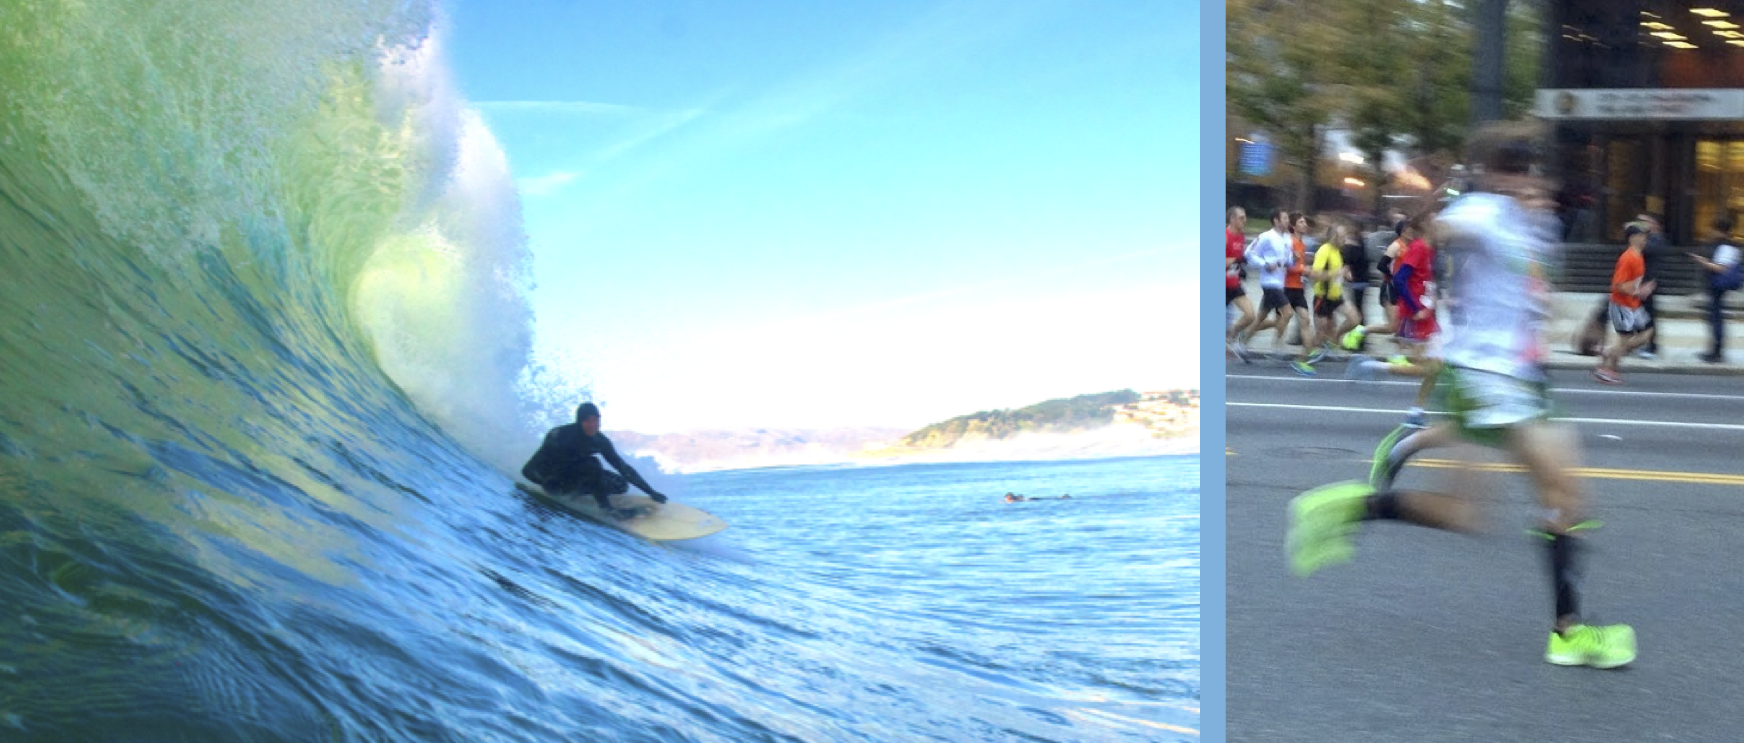
\includegraphics{./figures/brian_and_nick.png}

\end{frame}

\begin{frame}

\includegraphics{./figures/antsCollaborators2.png}

\(+\) \href{http://neuro.debian.net/pkgs/ants.html}{neurodebian},
\href{http://www.slicer.org/}{slicer},
\href{https://github.com/BRAINSia/BRAINSTools}{brainsfit},
\href{http://nipy.sourceforge.net/nipype/}{nipype},
\href{http://www.itk.org}{itk} and more \ldots{}

\end{frame}

\section{Why would you care?}\label{why-would-you-care}

\begin{frame}{Software for medical image analysis}

\begin{itemize}
\item
  \href{http://fsl.fmrib.ox.ac.uk/fsldownloads/}{FSL}
\item
  \href{http://www.fil.ion.ucl.ac.uk/spm/software/}{SPM}
\item
  \href{http://www.fil.ion.ucl.ac.uk/spm/software/}{FreeSurfer}
\item
  \href{http://mipav.cit.nih.gov}{MIPAV}
\item
  \href{https://afni.nimh.nih.gov/afni}{AFNI}
\item
  Slicer, Elastix, SimpleITK, ANTs \(\longleftrightarrow\)
  \href{http://www.itk.org}{Insight Toolkit}
\item
  Many more at \href{http://idoimaging.com}{idoimaging.com}
\end{itemize}

\end{frame}

\begin{frame}{International competitions}

\begin{itemize}
\item
  \href{http://www.ncbi.nlm.nih.gov/pubmed/19195496}{Klein 2009}: MRI
  brain registration
\item
  \href{http://empire10.isi.uu.nl}{EMPIRE 2010}: CT lung registration
\item
  \href{https://masi.vuse.vanderbilt.edu/workshop2012/index.php/Main_Page}{Multi-Atlas
  Label Challenge 2012}: MRI brain registration and segmentation
\item
  \href{https://masi.vuse.vanderbilt.edu/workshop2013/index.php/MICCAI_2013_SATA_Challenge_and_Workshop:Current_events}{SATA
  Challenge 2013}: MRI cardiac and canine hind leg registration
\item
  \href{http://martinos.org/qtim/miccai2013/}{BRATS 2013}: Multi-modal
  MRI brain segmentation
\item
  \href{http://www.cardiacatlas.org/web/stacom2014/moco-introduction}{STACOM
  2014 MoCo Challenge}: MRI cardiac motion estimation
\end{itemize}

\end{frame}

\section{ANTs lineage}\label{ants-lineage}

\begin{frame}{Image mapping and perception: 1877}

Francis Galton: \emph{Can we see criminality in the face?}

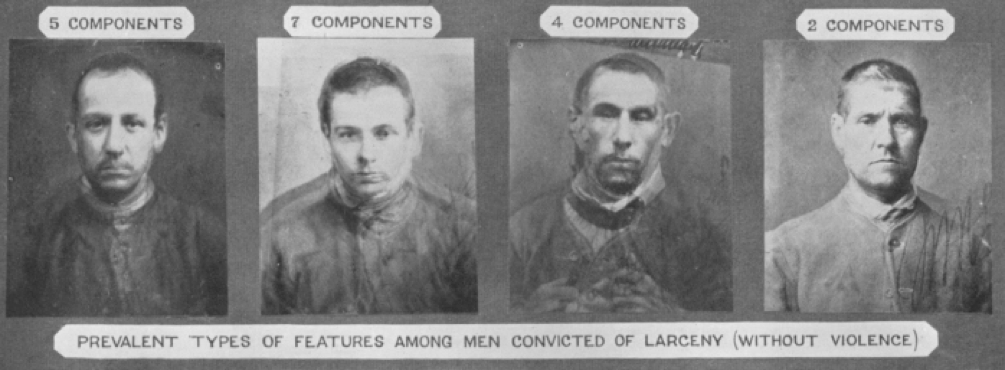
\includegraphics{./figures/galton.png}

\emph{What about syphilis, mental illness?}

\end{frame}

\begin{frame}{Speaking of criminality\ldots{}}

\emph{Can we say anything about the U.S. Congress?}

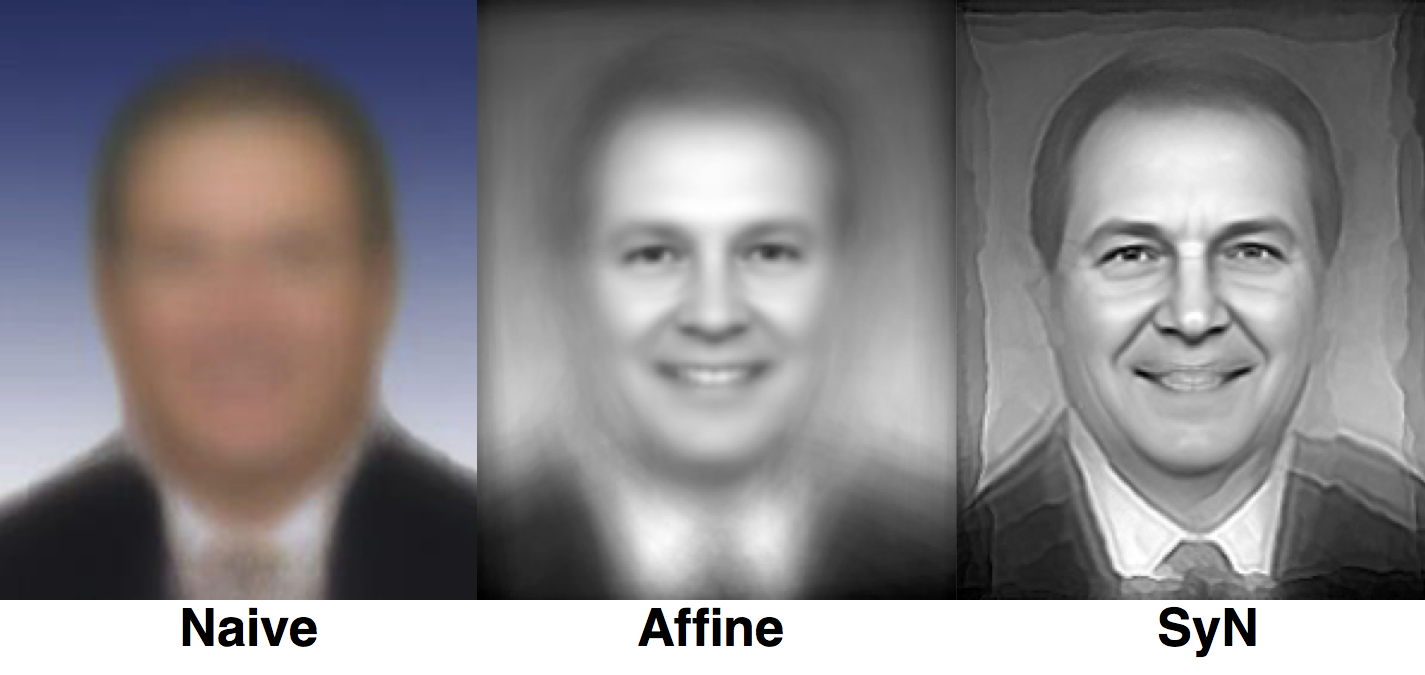
\includegraphics{./background/figures/congressPersons.png}

\textbf{Maybe they should have used
\href{https://github.com/ntustison/CongressionalFaceTemplates}{ANTs}?}

\end{frame}

\begin{frame}{Image mapping \& biology: 1917}

D'Arcy Thompson: \emph{Comparison of related forms}

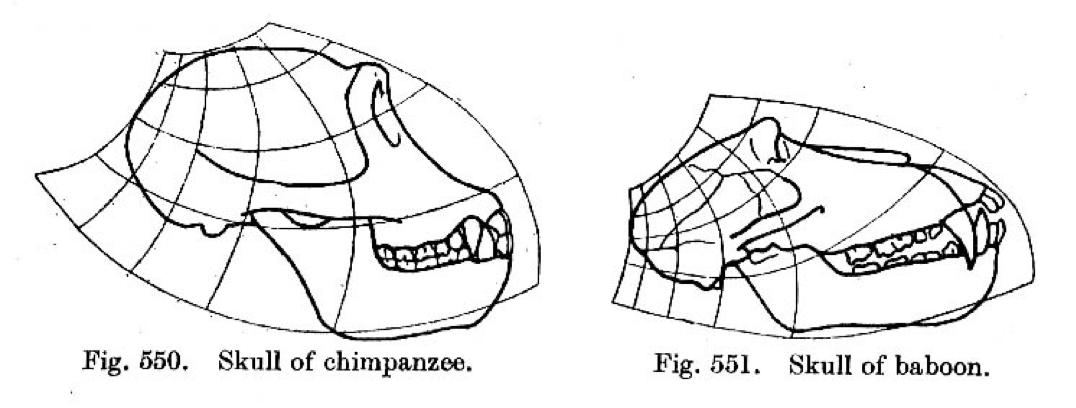
\includegraphics{./figures/dthompson.png} --\textgreater{}

\end{frame}

\begin{frame}{Image mapping \& biology: Current}

 \emph{Look where we are now!}
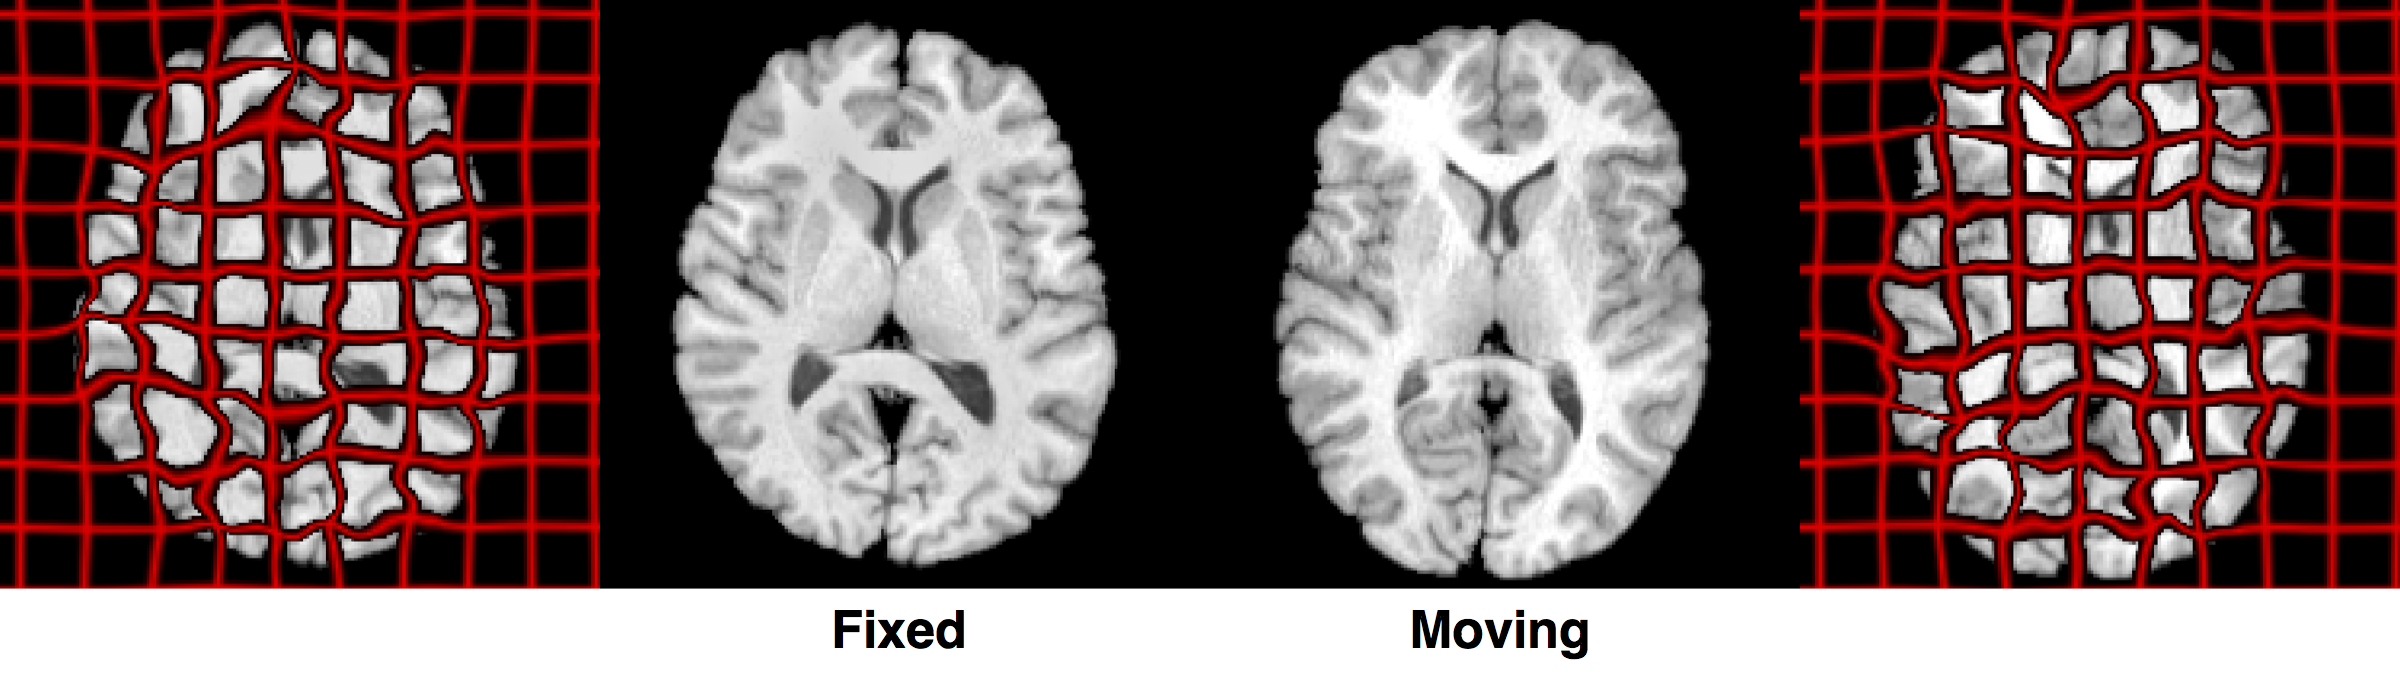
\includegraphics{./background/figures/r16xr85.png}

\end{frame}

\section{Major ANTs utilities}\label{major-ants-utilities}

\begin{frame}{Donoho?}

 \emph{``Papers are just advertisements for the science.''}

\end{frame}

\begin{frame}{Neuro tools}

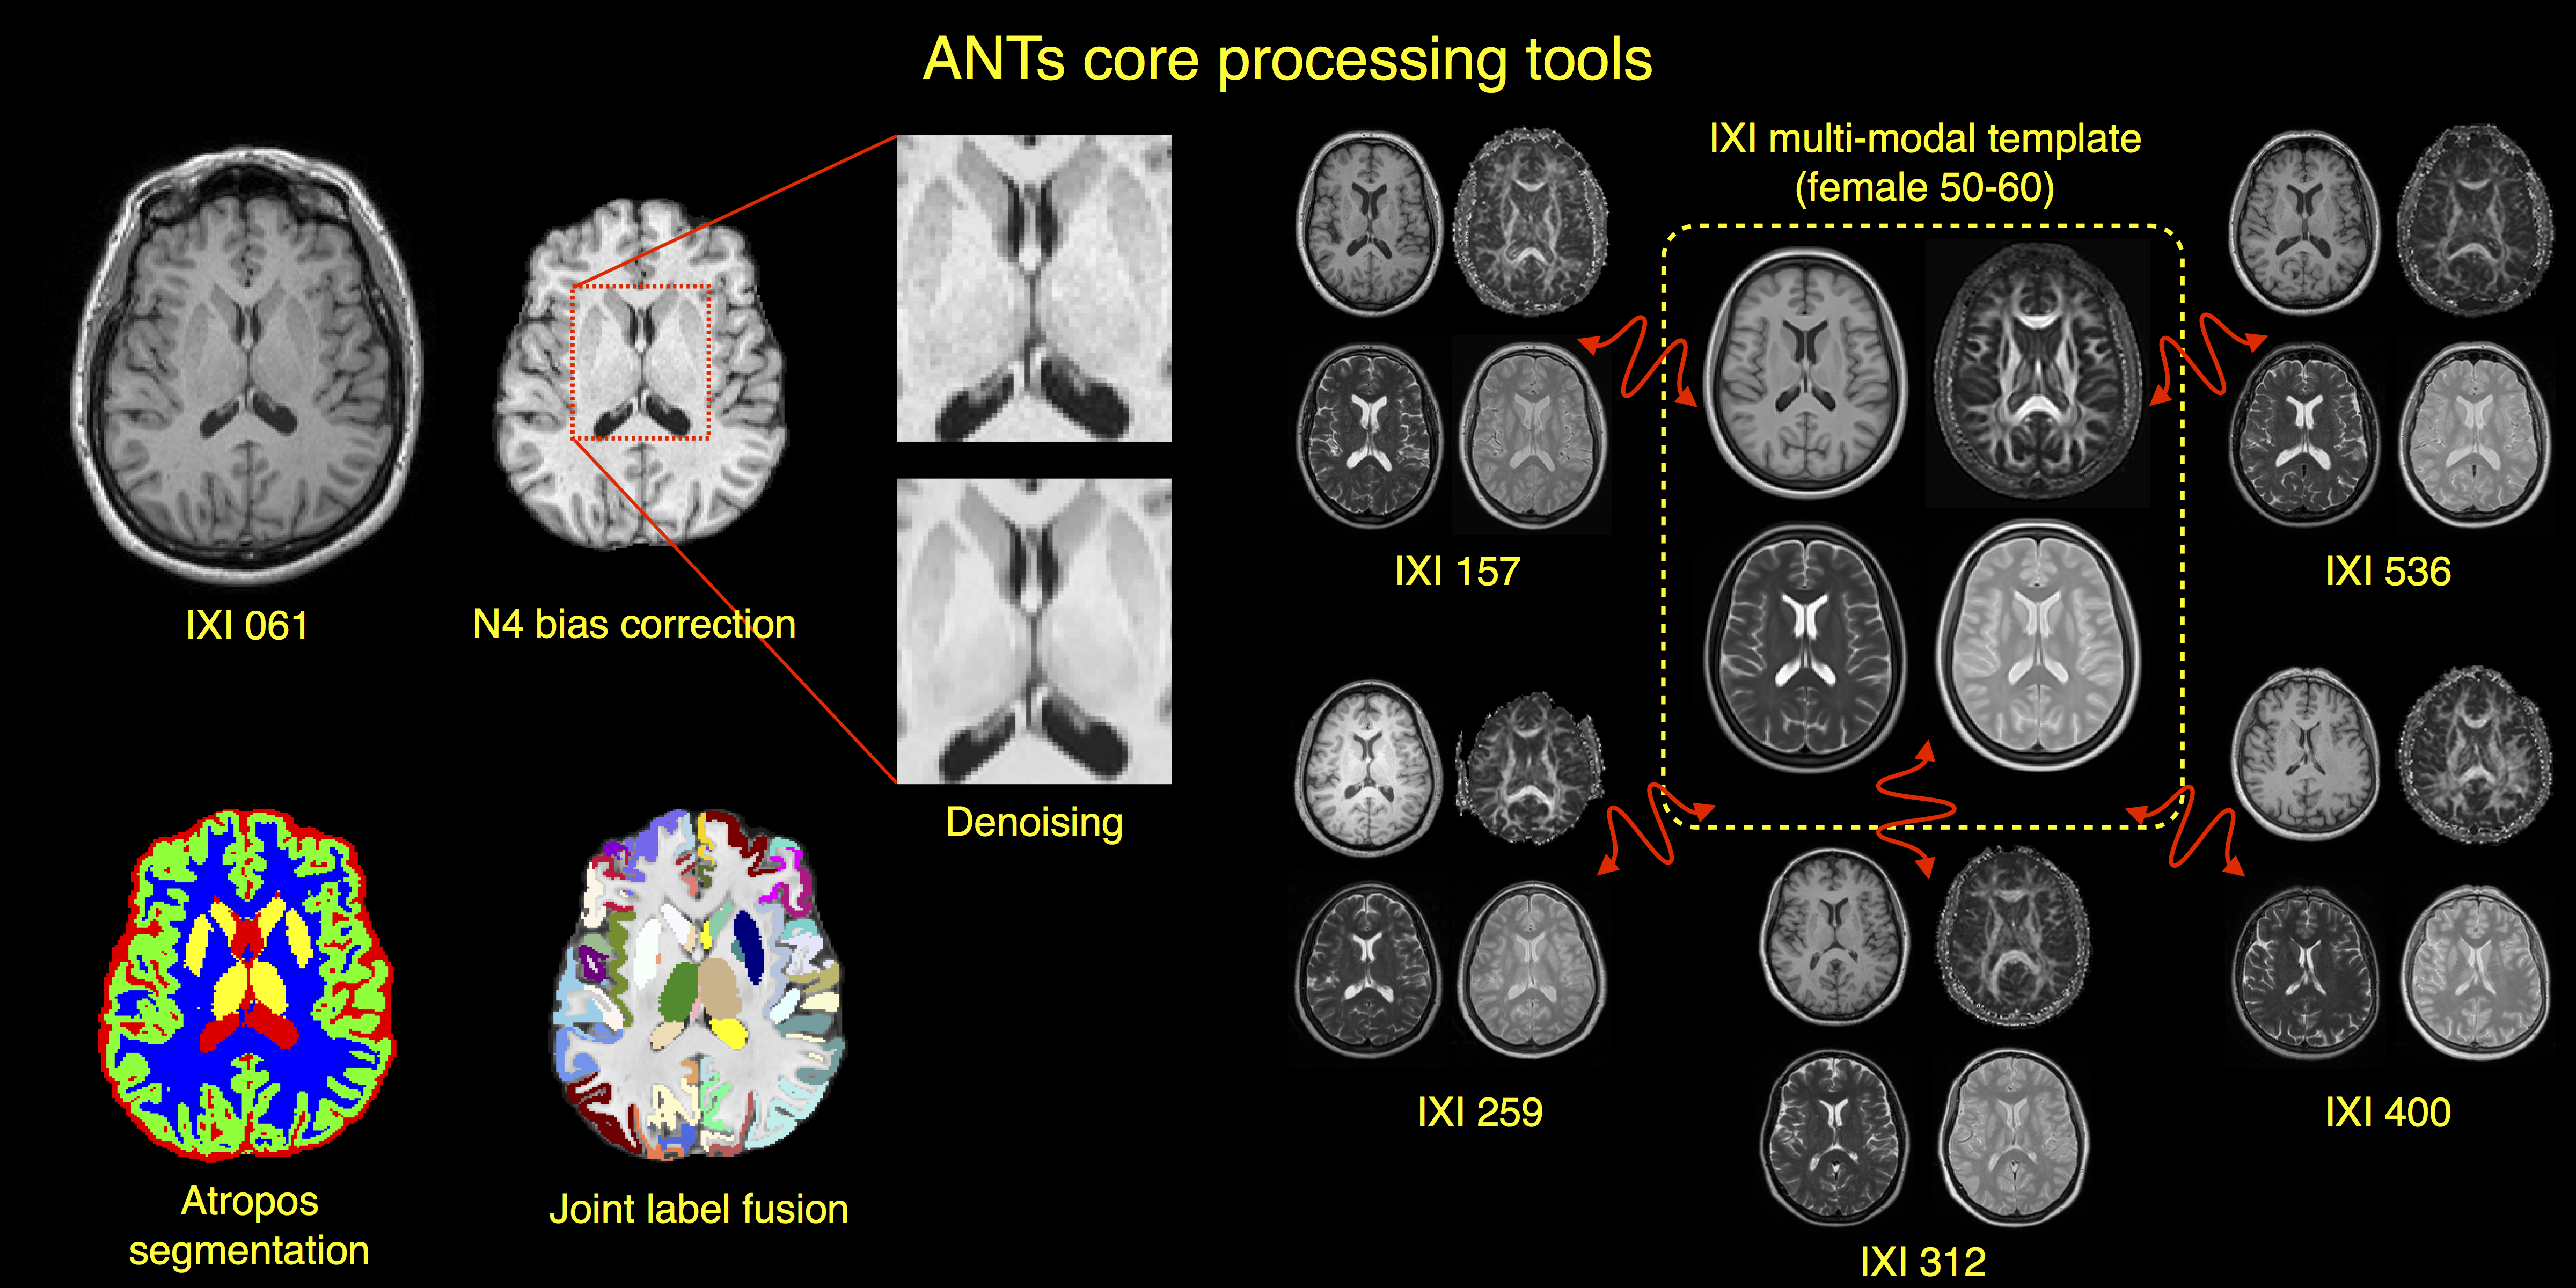
\includegraphics{./tools/figures/coreANtsToolsNeuro.png}

\end{frame}

\begin{frame}{Pulmonary tools}

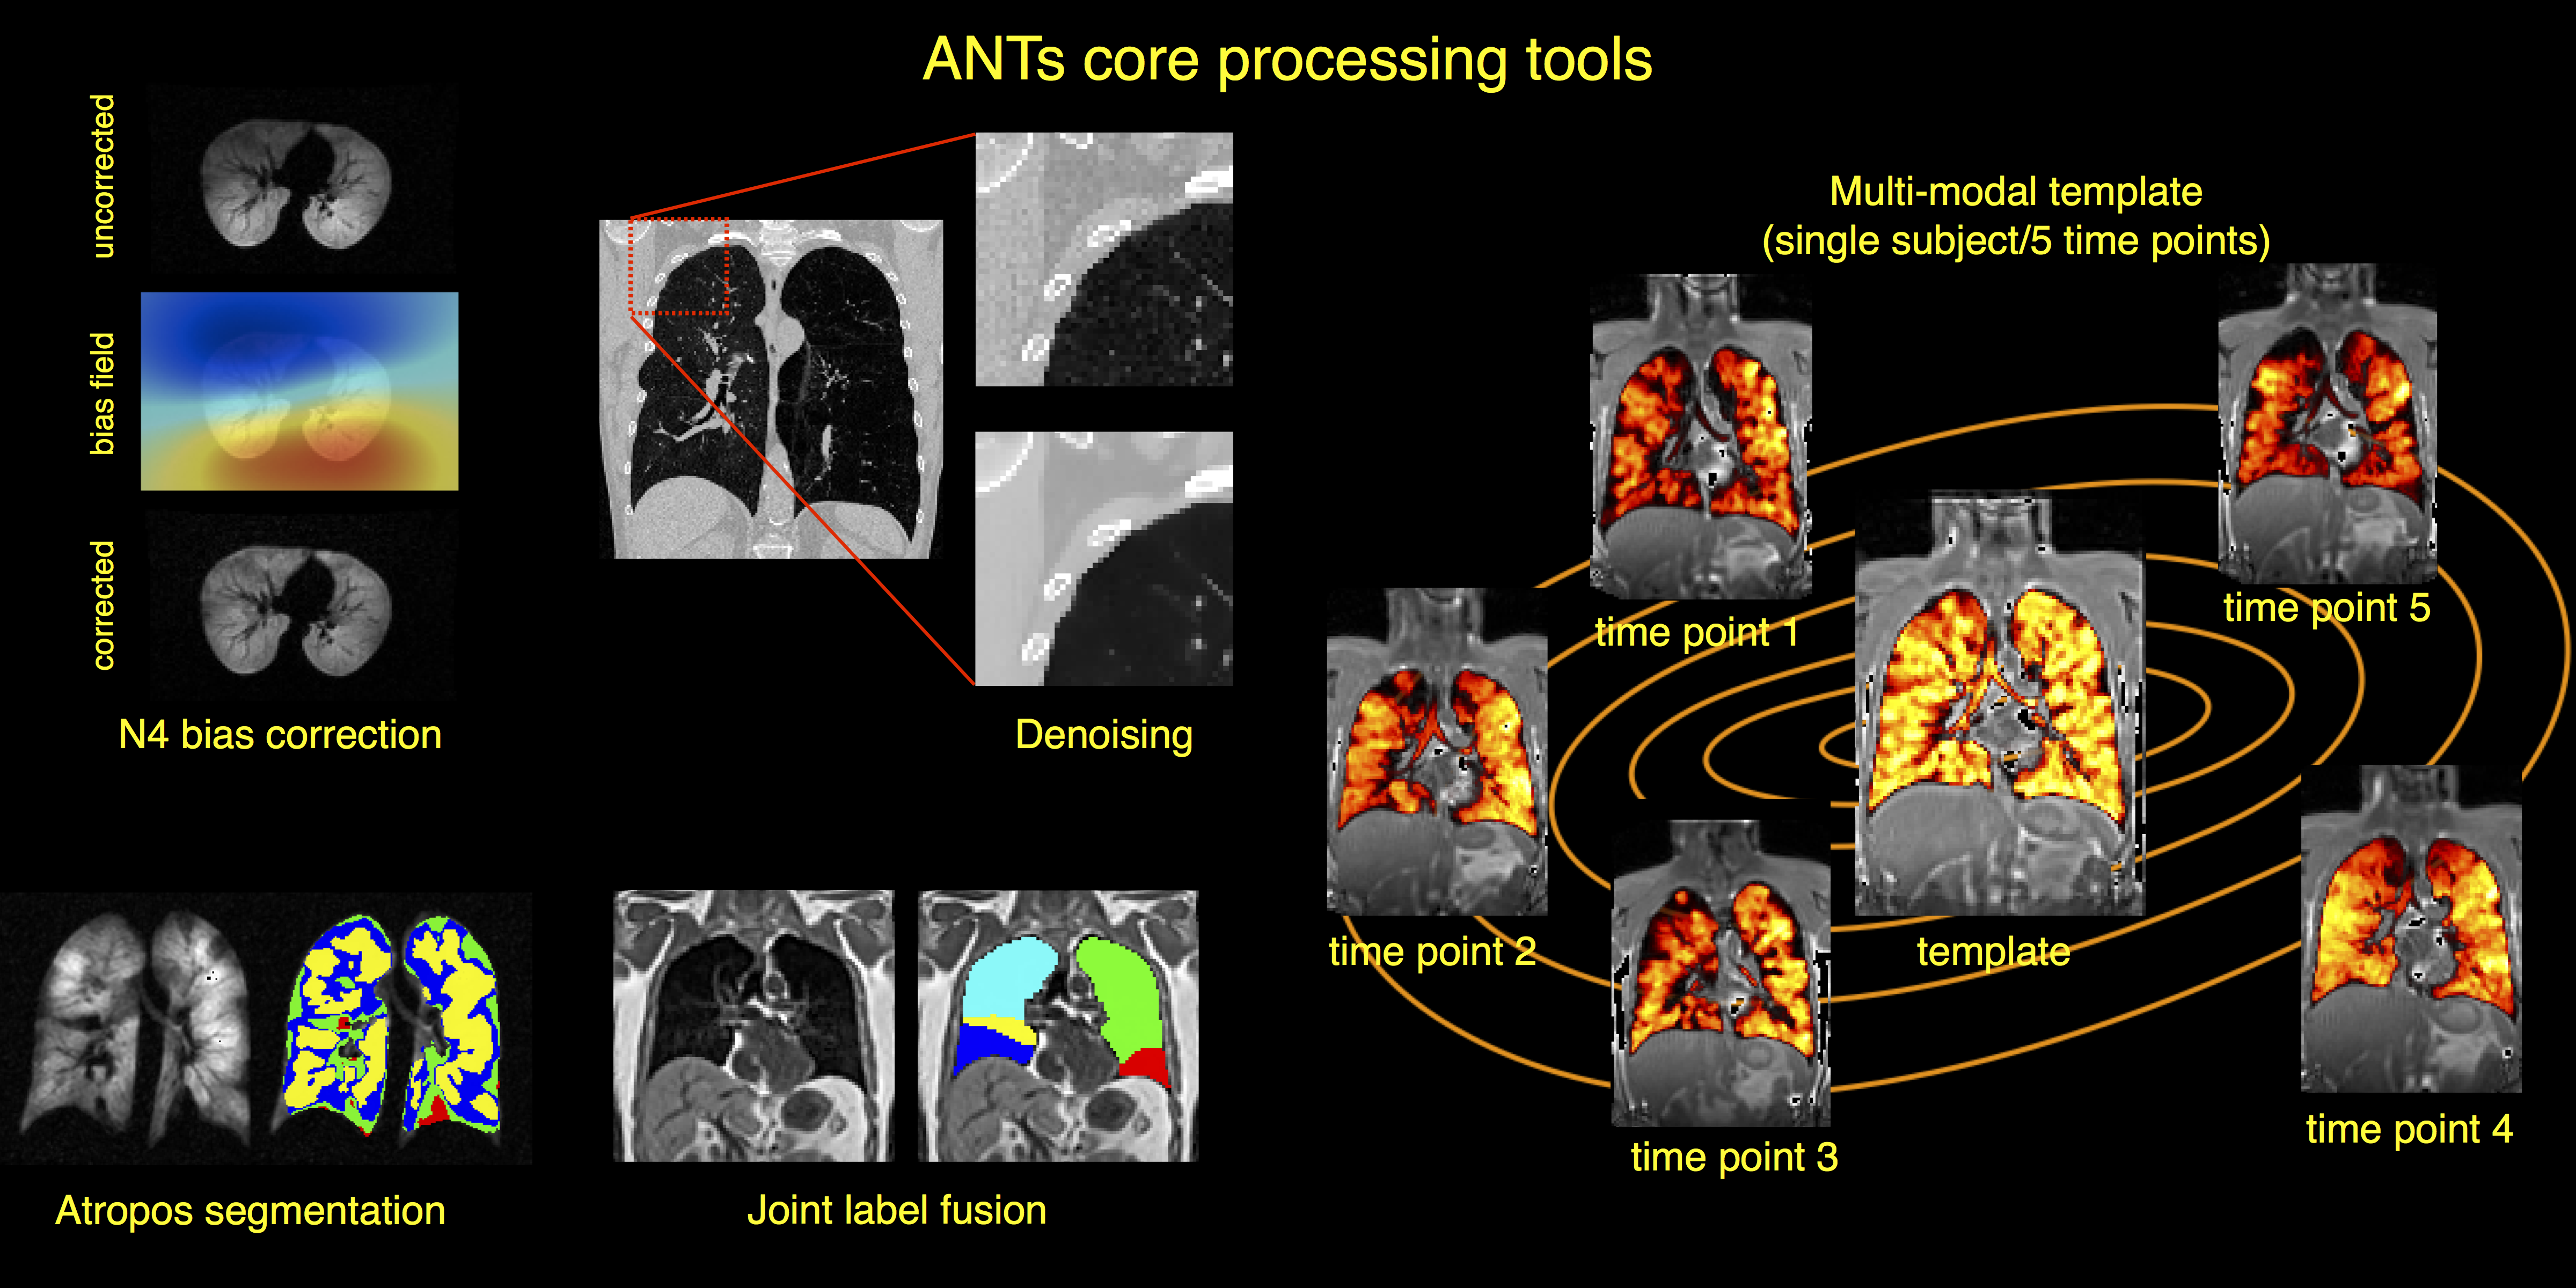
\includegraphics{./tools/figures/coreANtsToolsLung.png}

\end{frame}

\begin{frame}{Diffeomoprhisms: differentiable map with diff. inverse}

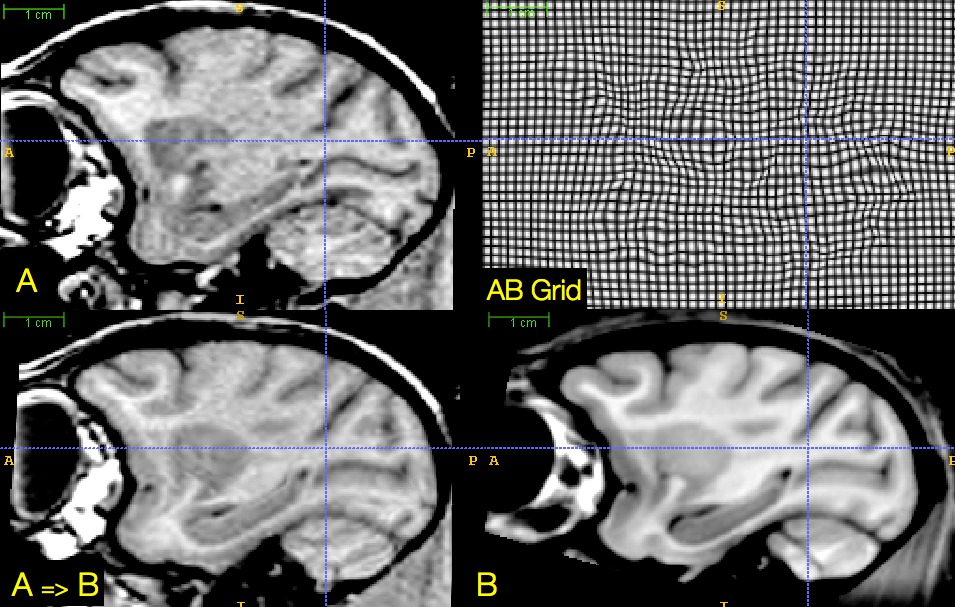
\includegraphics{./figures/highresdiffeos.jpg}

\end{frame}

\begin{frame}{Beyond original SyN}

\small

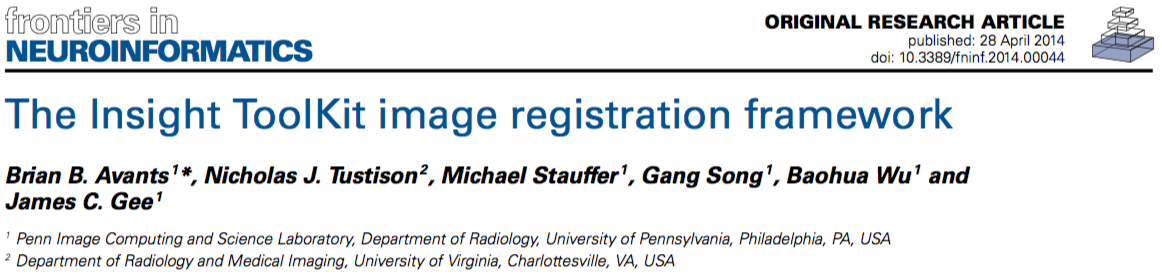
\includegraphics{./papers/figures/Frontiers_ITK.png}

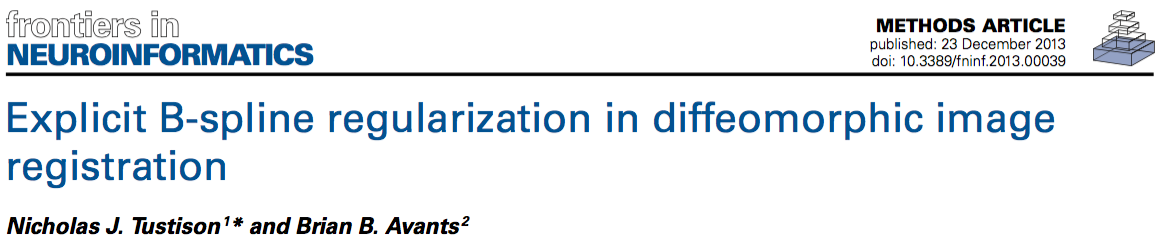
\includegraphics{./papers/figures/Frontiers_BSplineSyN.png}

\end{frame}

\begin{frame}[fragile]{\texttt{antsRegistration}}

\begin{Shaded}
\begin{Highlighting}[]
\NormalTok{$ }\KeywordTok{antsRegistration} \NormalTok{--help}

\KeywordTok{COMMAND}\NormalTok{:}
     \KeywordTok{antsRegistration}
          \KeywordTok{This} \NormalTok{program is a user-level registration application meant to utilize}
          \KeywordTok{ITKv4-only} \NormalTok{classes. The user can specify any number of }\StringTok{"stages"} \NormalTok{where a stage}
          \KeywordTok{consists} \NormalTok{of a transform}\KeywordTok{;} \KeywordTok{an} \NormalTok{image metric}\KeywordTok{;} \KeywordTok{and} \NormalTok{iterations, shrink factors, and}
          \KeywordTok{smoothing} \NormalTok{sigmas for each level.Note that dimensionality, metric, transform,}
          \KeywordTok{output}\NormalTok{, convergence, shrink-factors and smoothing-sigmas parameters are}
          \KeywordTok{mandatory.}

\KeywordTok{OPTIONS}\NormalTok{:}
     \KeywordTok{--version}
          \KeywordTok{Get} \NormalTok{Version Information.}

     \KeywordTok{-d}\NormalTok{, --dimensionality 2/3}
          \KeywordTok{This} \NormalTok{option forces the image to be treated as a specified-dimensional image. If}
          \KeywordTok{not} \NormalTok{specified, we try to infer the dimensionality from the input image.}

     \KeywordTok{-o}\NormalTok{, --output outputTransformPrefix}
                  \NormalTok{[}\KeywordTok{outputTransformPrefix}\NormalTok{,}\KeywordTok{<}\NormalTok{outputWarpedImage}\KeywordTok{>}\NormalTok{,}\KeywordTok{<}\NormalTok{outputInverseWarpedImage}\KeywordTok{>}\NormalTok{]}
          \KeywordTok{Specify} \NormalTok{the output transform prefix (output format is .nii.gz )}\KeywordTok{.} \KeywordTok{Optionally}\NormalTok{, one}
          \KeywordTok{can} \NormalTok{choose to warp the moving image to the fixed space and, if the inverse}
          \KeywordTok{transform} \NormalTok{exists, one can also output the warped fixed image. Note that only the}
          \KeywordTok{images} \NormalTok{specified in the first metric call are warped. Use antsApplyTransforms to}
          \KeywordTok{warp} \NormalTok{other images using the resultant transform(s)}\KeywordTok{.}

     \KeywordTok{-j}\NormalTok{, --save-state saveSateAsTransform}
          \KeywordTok{Specify} \NormalTok{the output file for the current state of the registration. The state}
          \KeywordTok{file} \NormalTok{is written to an hdf5 composite file. It is specially usefull if we want to}
          \KeywordTok{save} \NormalTok{the current state of a SyN registration to the disk, so we can load and}
          \KeywordTok{restore} \NormalTok{that later to continue the next registration process directly started}
          \KeywordTok{from} \NormalTok{the last saved state. The output file of this flag is the same as the}
          \KeywordTok{write-composite-transform}\NormalTok{, unless the last transform is a SyN transform. In that}
          \KeywordTok{case}\NormalTok{, the inverse displacement field of the SyN transform is also added to the}
          \NormalTok{output composite transform. Again notice that this file cannot be treated as a}
          \NormalTok{transform, and restore-state option must be used to load the written file by}
          \NormalTok{this flag.}

     \NormalTok{-k, --restore-state restoreStateAsATransform}
          \NormalTok{Specify the initial state of the registration which get immediately used to}
          \NormalTok{directly initialize the registration process. The flag is mutually exclusive}
          \NormalTok{with other intialization flags.If this flag is used, none of the}
          \NormalTok{initial-moving-transform and initial-fixed-transform cannot be used.}

     \NormalTok{-a, --write-composite-transform 1/(0)}
          \NormalTok{Boolean specifying whether or not the composite transform (and its inverse, if}
          \NormalTok{it exists) should be written to an hdf5 composite file. This is false by default}
          \NormalTok{so that only the transform for each stage is written to file.}
          \NormalTok{<VALUES>: 0}

     \NormalTok{-p, --print-similarity-measure-interval <unsignedIntegerValue>}
          \NormalTok{Prints out the CC similarity metric measure between the full-size input fixed}
          \NormalTok{and the transformed moving images at each iteration a value of 0 (the default)}
          \NormalTok{indicates that the full scale computation should not take placeany value greater}
          \NormalTok{than 0 represents the interval of full scale metric computation.}
          \NormalTok{<VALUES>: 0}

     \NormalTok{-v, --write-interval-volumes <unsignedIntegerValue>}
          \NormalTok{Writes out the output volume at each iteration. It helps to present the}
          \NormalTok{registration process as a short movie a value of 0 (the default) indicates that}
          \NormalTok{this option should not take placeany value greater than 0 represents the}
          \NormalTok{interval between the iterations which outputs are written to the disk.}
          \NormalTok{<VALUES>: 0}

     \NormalTok{-z, --collapse-output-transforms (1)/0}
          \NormalTok{Collapse output transforms. Specifically, enabling this option combines all}
          \NormalTok{adjacent transforms wherepossible. All adjacent linear transforms are written to}
          \NormalTok{disk}\KeywordTok{ in} \NormalTok{the forman itk affine transform }\KeywordTok{(}\NormalTok{called xxxGenericAffine.mat}\KeywordTok{).}
          \KeywordTok{Similarly}\NormalTok{, all adjacent displacement field transforms are combined when written}
          \KeywordTok{to} \NormalTok{disk (e.g. xxxWarp.nii.gz and xxxInverseWarp.nii.gz (if available))}\KeywordTok{.Also}\NormalTok{, an}
          \KeywordTok{output} \NormalTok{composite transform including the collapsed transforms is written to the}
          \KeywordTok{disk} \NormalTok{(called outputCollapsed(Inverse)}\KeywordTok{Composite}\NormalTok{)}\KeywordTok{.}
          \KeywordTok{<VALUES>}\NormalTok{: 1}

     \KeywordTok{-i}\NormalTok{, --initialize-transforms-per-stage (1)}\KeywordTok{/0}
          \KeywordTok{Initialize} \NormalTok{linear transforms from the previous stage. By enabling this option,}
          \KeywordTok{the} \NormalTok{current linear stage transform is directly intialized from the previous}
          \KeywordTok{stage}\StringTok{'s linear transform; this allows multiple linear stages to be run where}
\StringTok{          each stage directly updates the estimated linear transform from the previous}
\StringTok{          stage. (e.g. Translation -> Rigid -> Affine).}
\StringTok{          <VALUES>: 0}

\StringTok{     -n, --interpolation Linear}
\StringTok{                         NearestNeighbor}
\StringTok{                         MultiLabel[<sigma=imageSpacing>,<alpha=4.0>]}
\StringTok{                         Gaussian[<sigma=imageSpacing>,<alpha=1.0>]}
\StringTok{                         BSpline[<order=3>]}
\StringTok{                         CosineWindowedSinc}
\StringTok{                         WelchWindowedSinc}
\StringTok{                         HammingWindowedSinc}
\StringTok{                         LanczosWindowedSinc}
\StringTok{          Several interpolation options are available in ITK. These have all been made}
\StringTok{          available. Currently the interpolator choice is only used to warp (and possibly}
\StringTok{          inverse warp) the final output image(s).}

\StringTok{     -g, --restrict-deformation PxQxR}
\StringTok{          This option allows the user to restrict the optimization of the displacement}
\StringTok{          field, translation, rigid or affine transform on a per-component basis. For}
\StringTok{          example, if one wants to limit the deformation or rotation of 3-D volume to the}
\StringTok{          first two dimensions, this is possible by specifying a weight vector of '}\NormalTok{1x1x0}\StringTok{'}
\StringTok{          for a deformation field or '}\NormalTok{1x1x0x1x1x0}\StringTok{' for a rigid}
\StringTok{          transformation.Low-dimensional restriction only works if there are no preceding}
\StringTok{          transformations.}

\StringTok{     -q, --initial-fixed-transform initialTransform}
\StringTok{                                   [initialTransform,<useInverse>]}
\StringTok{                                   [fixedImage,movingImage,initializationFeature]}
\StringTok{          Specify the initial fixed transform(s) which get immediately incorporated into}
\StringTok{          the composite transform. The order of the transforms is stack-esque in that the}
\StringTok{          last transform specified on the command line is the first to be applied. In}
\StringTok{          addition to initialization with ITK transforms, the user can perform an initial}
\StringTok{          translation alignment by specifying the fixed and moving images and selecting an}
\StringTok{          initialization feature. These features include using the geometric center of the}
\StringTok{          images (=0), the image intensities (=1), or the origin of the images (=2).}

\StringTok{     -r, --initial-moving-transform initialTransform}
\StringTok{                                    [initialTransform,<useInverse>]}
\StringTok{                                    [fixedImage,movingImage,initializationFeature]}
\StringTok{          Specify the initial moving transform(s) which get immediately incorporated into}
\StringTok{          the composite transform. The order of the transforms is stack-esque in that the}
\StringTok{          last transform specified on the command line is the first to be applied. In}
\StringTok{          addition to initialization with ITK transforms, the user can perform an initial}
\StringTok{          translation alignment by specifying the fixed and moving images and selecting an}
\StringTok{          initialization feature. These features include using the geometric center of the}
\StringTok{          images (=0), the image intensities (=1), or the origin of the images (=2).}

\StringTok{     -m, --metric CC[fixedImage,movingImage,metricWeight,radius,<samplingStrategy=\{None,Regular,Random\}>,<samplingPercentage=[0,1]>]}
\StringTok{                  MI[fixedImage,movingImage,metricWeight,numberOfBins,<samplingStrategy=\{None,Regular,Random\}>,<samplingPercentage=[0,1]>]}
\StringTok{                  Mattes[fixedImage,movingImage,metricWeight,numberOfBins,<samplingStrategy=\{None,Regular,Random\}>,<samplingPercentage=[0,1]>]}
\StringTok{                  MeanSquares[fixedImage,movingImage,metricWeight,radius=NA,<samplingStrategy=\{None,Regular,Random\}>,<samplingPercentage=[0,1]>]}
\StringTok{                  Demons[fixedImage,movingImage,metricWeight,radius=NA,<samplingStrategy=\{None,Regular,Random\}>,<samplingPercentage=[0,1]>]}
\StringTok{                  GC[fixedImage,movingImage,metricWeight,radius=NA,<samplingStrategy=\{None,Regular,Random\}>,<samplingPercentage=[0,1]>]}
\StringTok{                  ICP[fixedPointSet,movingPointSet,metricWeight,<samplingPercentage=[0,1]>,<boundaryPointsOnly=0>]}
\StringTok{                  PSE[fixedPointSet,movingPointSet,metricWeight,<samplingPercentage=[0,1]>,<boundaryPointsOnly=0>,<pointSetSigma=1>,<kNeighborhood=50>]}
\StringTok{                  JHCT[fixedPointSet,movingPointSet,metricWeight,<samplingPercentage=[0,1]>,<boundaryPointsOnly=0>,<pointSetSigma=1>,<kNeighborhood=50>,<alpha=1.1>,<useAnisotropicCovariances=1>]}
\StringTok{                  IGDM[fixedImage,movingImage,metricWeight,fixedMask,movingMask,<neighborhoodRadius=0x0>,<intensitySigma=0>,<distanceSigma=0>,<kNeighborhood=1>,<gradientSigma=1>]}
\StringTok{          These image metrics are available--- CC: ANTS neighborhood cross correlation,}
\StringTok{          MI: Mutual information, Demons: (Thirion), MeanSquares, and GC: Global}
\StringTok{          Correlation. The "metricWeight" variable is used to modulate the per stage}
\StringTok{          weighting of the metrics. The metrics can also employ a sampling strategy}
\StringTok{          defined by a sampling percentage. The sampling strategy defaults to '}\NormalTok{None}\StringTok{' (aka}
\StringTok{          a dense sampling of one sample per voxel), otherwise it defines a point set over}
\StringTok{          which to optimize the metric. The point set can be on a regular lattice or a}
\StringTok{          random lattice of points slightly perturbed to minimize aliasing artifacts.}
\StringTok{          samplingPercentage defines the fraction of points to select from the domain. In}
\StringTok{          addition, three point set metrics are available: Euclidean (ICP), Point-set}
\StringTok{          expectation (PSE), and Jensen-Havrda-Charvet-Tsallis (JHCT).}

\StringTok{     -t, --transform Rigid[gradientStep]}
\StringTok{                     Affine[gradientStep]}
\StringTok{                     CompositeAffine[gradientStep]}
\StringTok{                     Similarity[gradientStep]}
\StringTok{                     Translation[gradientStep]}
\StringTok{                     BSpline[gradientStep,meshSizeAtBaseLevel]}
\StringTok{                     GaussianDisplacementField[gradientStep,updateFieldVarianceInVoxelSpace,totalFieldVarianceInVoxelSpace]}
\StringTok{                     BSplineDisplacementField[gradientStep,updateFieldMeshSizeAtBaseLevel,totalFieldMeshSizeAtBaseLevel,<splineOrder=3>]}
\StringTok{                     TimeVaryingVelocityField[gradientStep,numberOfTimeIndices,updateFieldVarianceInVoxelSpace,updateFieldTimeVariance,totalFieldVarianceInVoxelSpace,totalFieldTimeVariance]}
\StringTok{                     TimeVaryingBSplineVelocityField[gradientStep,velocityFieldMeshSize,<numberOfTimePointSamples=4>,<splineOrder=3>]}
\StringTok{                     SyN[gradientStep,updateFieldVarianceInVoxelSpace,totalFieldVarianceInVoxelSpace]}
\StringTok{                     BSplineSyN[gradientStep,updateFieldMeshSizeAtBaseLevel,totalFieldMeshSizeAtBaseLevel,<splineOrder=3>]}
\StringTok{                     Exponential[gradientStep,updateFieldVarianceInVoxelSpace,velocityFieldVarianceInVoxelSpace,<numberOfIntegrationSteps>]}
\StringTok{                     BSplineExponential[gradientStep,updateFieldMeshSizeAtBaseLevel,velocityFieldMeshSizeAtBaseLevel,<numberOfIntegrationSteps>,<splineOrder=3>]}
\StringTok{          Several transform options are available. The gradientStep or learningRate}
\StringTok{          characterizes the gradient descent optimization and is scaled appropriately for}
\StringTok{          each transform using the shift scales estimator. Subsequent parameters are}
\StringTok{          transform-specific and can be determined from the usage. For the B-spline}
\StringTok{          transforms one can also specify the smoothing in terms of spline distance (i.e.}
\StringTok{          knot spacing).}

\StringTok{     -c, --convergence MxNxO}
\StringTok{                       [MxNxO,<convergenceThreshold=1e-6>,<convergenceWindowSize=10>]}
\StringTok{          Convergence is determined from the number of iterations per level and is}
\StringTok{          determined by fitting a line to the normalized energy profile of the last N}
\StringTok{          iterations (where N is specified by the window size) and determining the slope}
\StringTok{          which is then compared with the convergence threshold.}

\StringTok{     -s, --smoothing-sigmas MxNxO...}
\StringTok{          Specify the sigma of gaussian smoothing at each level. Units are given in terms}
\StringTok{          of voxels ('}\NormalTok{vox}\StringTok{') or physical spacing ('}\NormalTok{mm}\StringTok{'). Example usage is '}\NormalTok{4x2x1mm}\StringTok{' and}
\StringTok{          '}\NormalTok{4x2x1vox}\StringTok{' where no units implies voxel spacing.}

\StringTok{     -f, --shrink-factors MxNxO...}
\StringTok{          Specify the shrink factor for the virtual domain (typically the fixed image) at}
\StringTok{          each level.}

\StringTok{     -u, --use-histogram-matching}
\StringTok{          Histogram match the images before registration.}

\StringTok{     -l, --use-estimate-learning-rate-once}
\StringTok{          turn on the option that lets you estimate the learning rate step size only at}
\StringTok{          the beginning of each level. * useful as a second stage of fine-scale}
\StringTok{          registration.}

\StringTok{     -w, --winsorize-image-intensities [lowerQuantile,upperQuantile]}
\StringTok{          Winsorize data based on specified quantiles.}

\StringTok{     -x, --masks [fixedImageMask,movingImageMask]}
\StringTok{          Image masks to limit voxels considered by the metric.}

\StringTok{     --float}
\StringTok{          Use '}\NormalTok{float}\StringTok{' instead of '}\NormalTok{double}\StringTok{' for computations.}
\StringTok{          <VALUES>: 0}

\StringTok{     -v, --verbose (0)/1}
\StringTok{          Verbose output.}

\StringTok{     -h}
\StringTok{          Print the help menu (short version).}

\StringTok{     --help}
\StringTok{          Print the help menu. Will also print values used on the current command line}
\StringTok{          call.}
\end{Highlighting}
\end{Shaded}

\end{frame}

\begin{frame}{Template building: creating the average Joe}

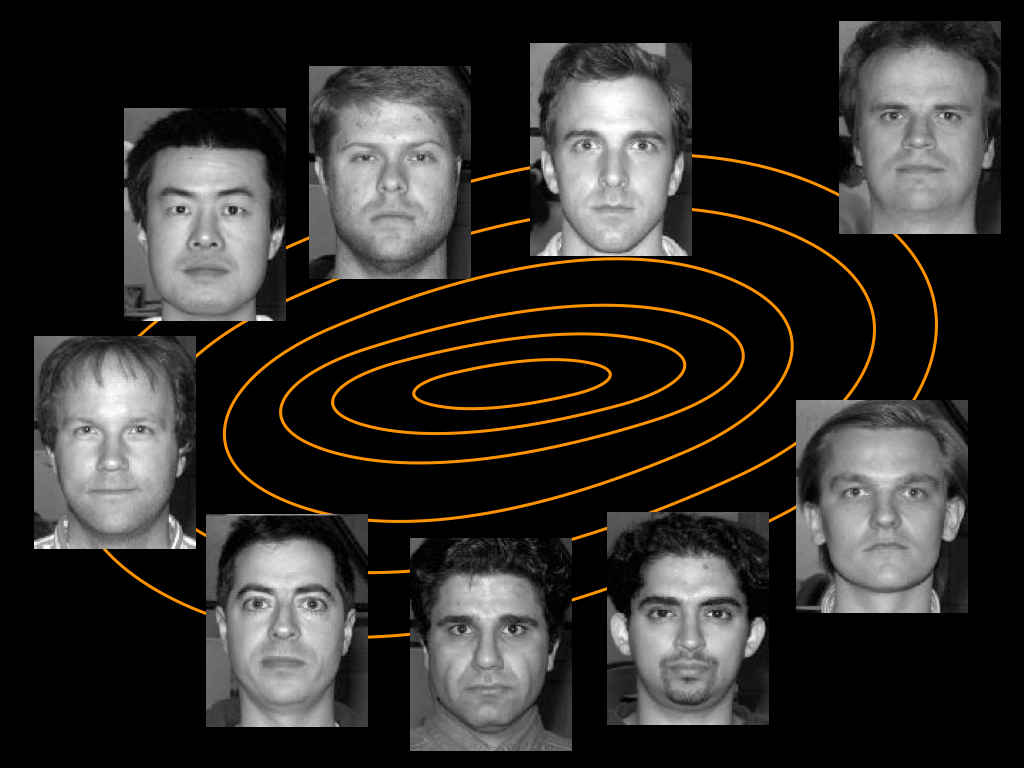
\includegraphics{./papers/figures/template0.jpg}

\end{frame}

\begin{frame}{``Attractiveness'' \(\rightarrow\) mental processing?}

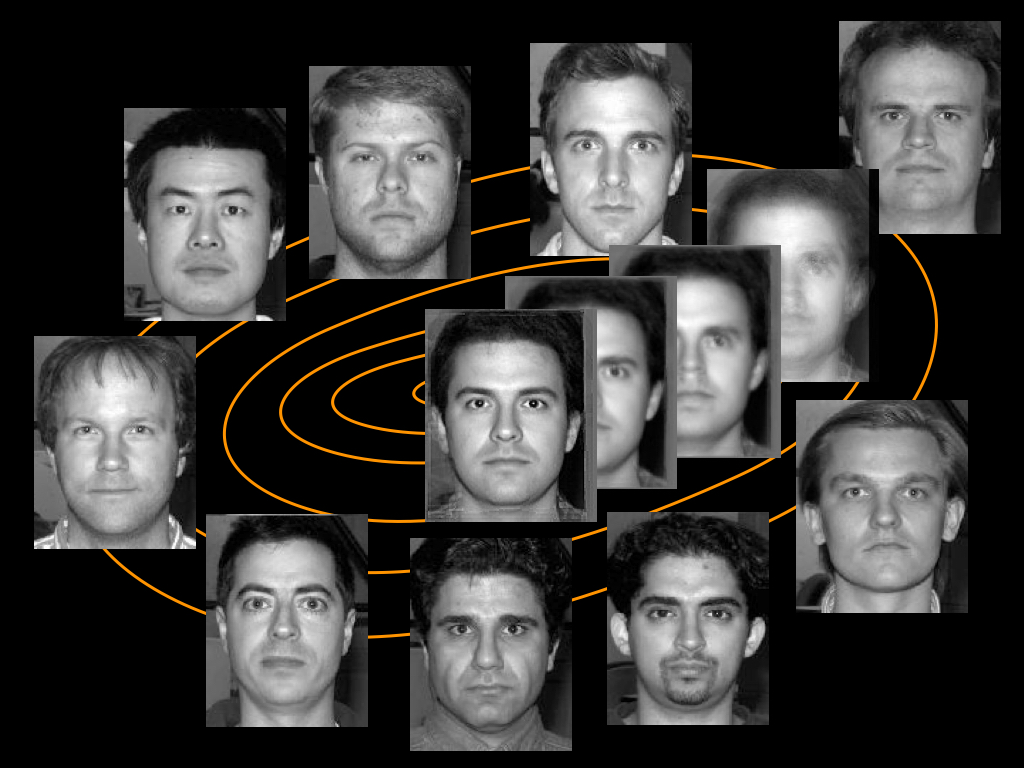
\includegraphics{./papers/figures/template1.jpg}

\end{frame}

\begin{frame}{What about brains?}

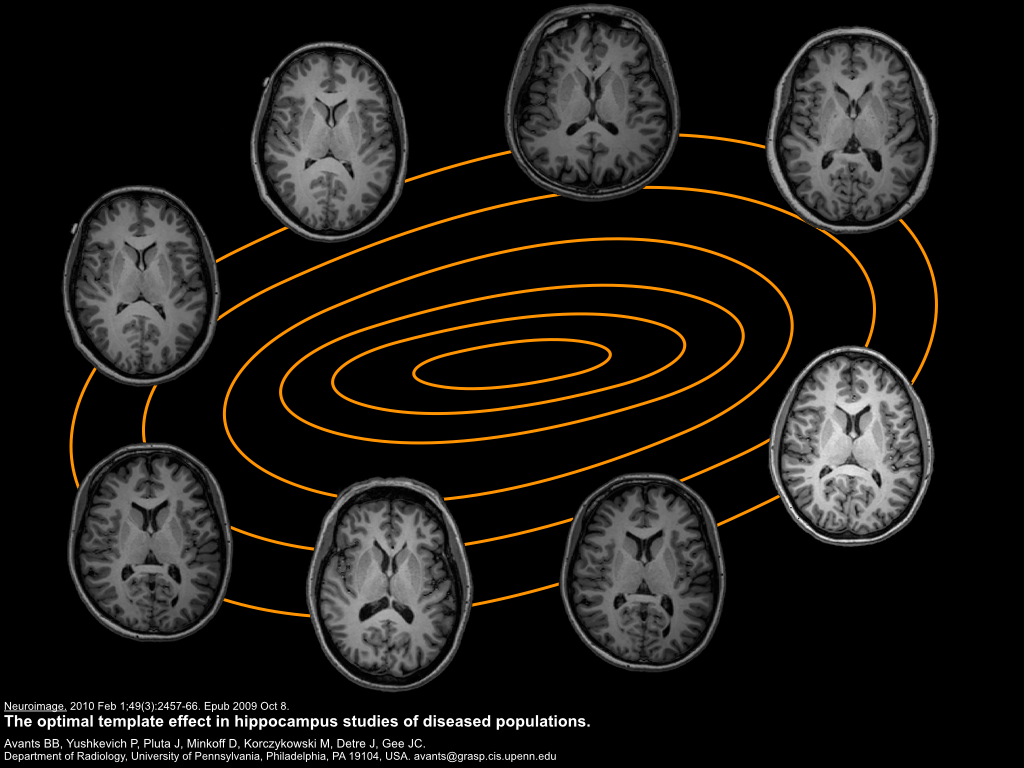
\includegraphics{./papers/figures/template3.jpg}

\end{frame}

\begin{frame}{Templates facilitate computation}

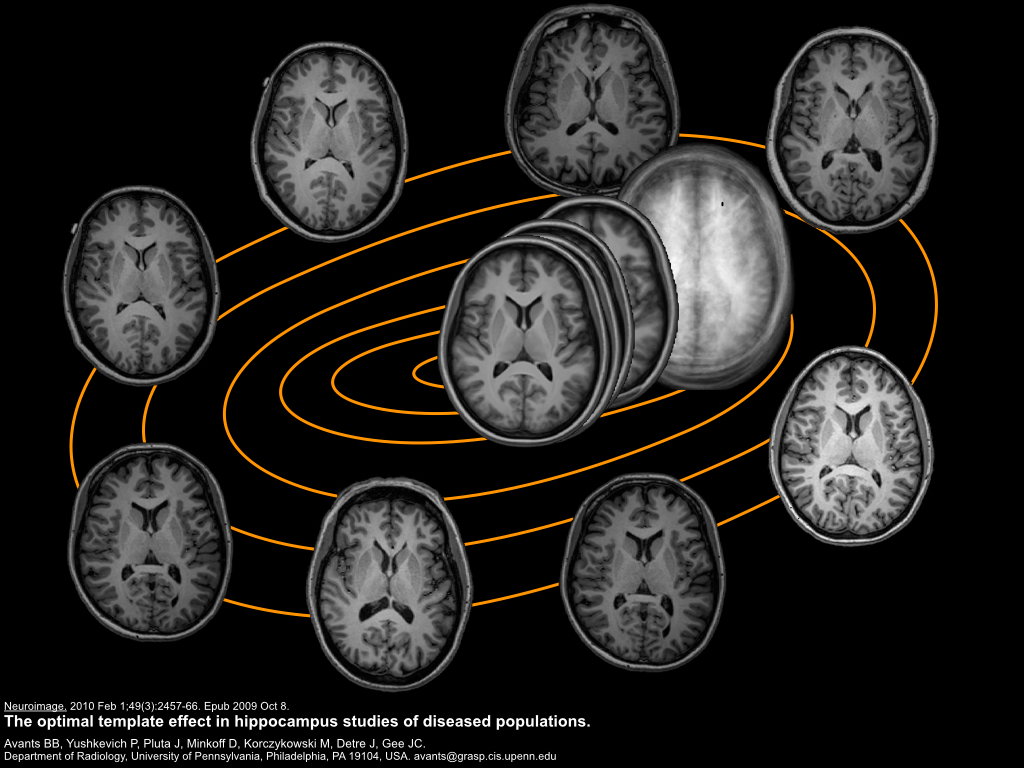
\includegraphics{./papers/figures/template4.jpg}

\end{frame}

\begin{frame}{Gender discernibility?}

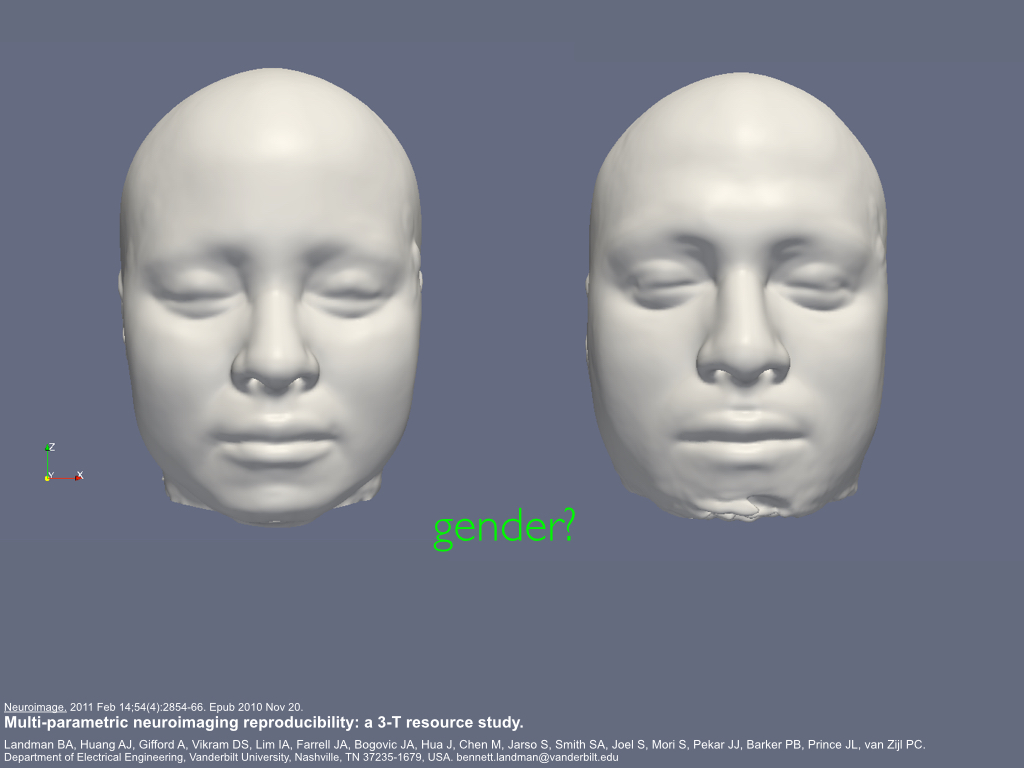
\includegraphics{./papers/figures/template5.jpg}

\end{frame}

\begin{frame}[fragile]{\texttt{antsMultivariateTemplateConstruction.sh}}

\begin{Shaded}
\begin{Highlighting}[]
\NormalTok{$ }\KeywordTok{antsMultivariateTemplateConstruction.sh}

\KeywordTok{Usage}\NormalTok{:}

\KeywordTok{antsMultivariateTemplateConstruction.sh} \NormalTok{-d ImageDimension -o OUTPREFIX }\KeywordTok{<}\NormalTok{other options}\KeywordTok{>} \KeywordTok{<}\NormalTok{images}\KeywordTok{>}

\KeywordTok{Compulsory} \NormalTok{arguments (minimal command line requires SGE cluster, otherwise use -c }\KeywordTok{&} \KeywordTok{-j} \NormalTok{options)}\KeywordTok{:}

     \KeywordTok{-d}\NormalTok{:  ImageDimension: 2 or 3 (for 2 or 3 dimensional registration of single volume)}
   \KeywordTok{ImageDimension}\NormalTok{: 4 (for template generation of time-series data)}

     \KeywordTok{-o}\NormalTok{:  OUTPREFIX}\KeywordTok{;} \KeywordTok{A} \NormalTok{prefix that is prepended to all output files.}

\KeywordTok{<images>}  \NormalTok{List of images in the current directory, eg *_t1.nii.gz. Should be at the end}
          \KeywordTok{of} \NormalTok{the command.  Optionally, one can specify a .csv or .txt file where each}
          \KeywordTok{line} \NormalTok{is the location of the input image.  One can also specify more than}
          \KeywordTok{one} \NormalTok{file for each image for multi-modal template construction (e.g. t1 and t2)}\KeywordTok{.}
          \KeywordTok{For} \NormalTok{the multi-modal case, the templates will be consecutively numbered (e.g.}
          \KeywordTok{template0.nii.gz}\NormalTok{, template1.nii.gz, ...)}\KeywordTok{.}

\KeywordTok{NB}\NormalTok{: All images to be added to the template should be in the same directory, and this script}
\KeywordTok{should} \NormalTok{be invoked from that directory.}

\KeywordTok{Optional} \NormalTok{arguments:}

     \KeywordTok{-c}\NormalTok{:  Control for parallel computation (default 1) }\KeywordTok{--} \NormalTok{0 == run serially,  1 == SGE qsub,}
          \KeywordTok{2} \NormalTok{== use PEXEC (localhost), }\KeywordTok{3} \NormalTok{== Apple XGrid, 4 == PBS qsub, 5 == SLURM}

     \KeywordTok{-g}\NormalTok{:  Gradient step size (default 0.25) }\KeywordTok{--} \NormalTok{smaller in magnitude results in more cautious steps}

     \KeywordTok{-i}\NormalTok{:  Iteration limit (default 4) }\KeywordTok{--} \NormalTok{iterations of the template construction (Iteration limit)}\KeywordTok{*NumImages} \NormalTok{registrations.}

     \KeywordTok{-j}\NormalTok{:  Number of cpu cores to use (default 2}\KeywordTok{;} \KeywordTok{--} \NormalTok{requires }\StringTok{"-c 2"}\NormalTok{)}

     \KeywordTok{-k}\NormalTok{:  Number of modalities used to construct the template (default 1)}

     \KeywordTok{-w}\NormalTok{:  Modality weights used in the similarity metric (default = 1) }\KeywordTok{---} \NormalTok{specified as e.g. 1x0.5x0.75}

     \KeywordTok{-m}\NormalTok{:  Max-iterations in each registration}

     \KeywordTok{-n}\NormalTok{:  N4BiasFieldCorrection of moving image (default 1) }\KeywordTok{--} \NormalTok{0 == off, 1 == on}

     \KeywordTok{-p}\NormalTok{:  Commands to prepend to job scripts (e.g., change into appropriate directory, set paths, etc)}

     \KeywordTok{-r}\NormalTok{:  Do rigid-body registration of inputs before creating template (default 0) }\KeywordTok{--} \NormalTok{0 == off 1 == on. Only useful when}
          \KeywordTok{you} \NormalTok{do not have an initial template}

     \KeywordTok{-s}\NormalTok{:  Type of similarity metric used for registration.}

     \KeywordTok{-t}\NormalTok{:  Type of transformation model used for registration.}

     \KeywordTok{-x}\NormalTok{:  XGrid arguments (e.g., -x }\StringTok{"-p password -h controlhost"}\NormalTok{)}

     \KeywordTok{-y}\NormalTok{:  Update the template with the full affine transform (default 1)}\KeywordTok{.} \KeywordTok{If} \NormalTok{0, the rigid}
          \KeywordTok{component} \NormalTok{of the affine transform will not be used to update the template. If your}
          \KeywordTok{template} \NormalTok{drifts in translation or orientation try -y 0.}

     \KeywordTok{-z}\NormalTok{:  Use this this volume as the target of all inputs. When not used, the script}
          \KeywordTok{will} \NormalTok{create an unbiased starting point by averaging all inputs. Use the full path!}

     \KeywordTok{-b}\NormalTok{:  Boolean for saving iteration output to directories (default = 0)}\KeywordTok{.}

\KeywordTok{Example}\NormalTok{:}

\KeywordTok{antsMultivariateTemplateConstruction.sh} \NormalTok{-d 3 -m 30x50x20 -t GR -s CC -c 1 -o MY -z InitialTemplate.nii.gz  *RF*T1x.nii.gz}

\KeywordTok{-} \NormalTok{In this example 30x50x20 iterations per registration are used for template creation (that is the default)}
\KeywordTok{-} \NormalTok{Greedy-SyN and CC are the metrics to guide the mapping.}
\KeywordTok{-} \NormalTok{Output is prepended with MY and the initial template is InitialTemplate.nii.gz (optional)}\KeywordTok{.}
\KeywordTok{-} \NormalTok{The -c option is set to 1, which will result in using the Sun Grid Engine (SGE) }\KeywordTok{to} \NormalTok{distribute the computation.}
\KeywordTok{-} \NormalTok{if you do not have SGE, read the help for multi-core computation on the local machine, or Apple X-grid options.}

\KeywordTok{--------------------------------------------------------------------------------------}
\KeywordTok{ANTS} \NormalTok{was created by:}
\KeywordTok{--------------------------------------------------------------------------------------}
\KeywordTok{Brian} \NormalTok{B. Avants, Nick Tustison and Gang Song}
\KeywordTok{Penn} \NormalTok{Image Computing And Science Laboratory}
\KeywordTok{University} \NormalTok{of Pennsylvania}

\KeywordTok{Please} \NormalTok{reference http://www.ncbi.nlm.nih.gov/pubmed/20851191 when employing this script}
\KeywordTok{in} \KeywordTok{your} \NormalTok{studies. A reproducible evaluation of ANTs similarity metric performance in}
\KeywordTok{brain} \NormalTok{image registration:}

\KeywordTok{*} \NormalTok{Avants BB, Tustison NJ, Song G, Cook PA, Klein A, Gee JC. Neuroimage, 2011.}

\KeywordTok{Also} \NormalTok{see http://www.ncbi.nlm.nih.gov/pubmed/19818860 for more details.}

\KeywordTok{The} \NormalTok{script has been updated and improved since this publication.}

\KeywordTok{--------------------------------------------------------------------------------------}
\KeywordTok{script} \NormalTok{adapted by N.M. van Strien, http://www.mri-tutorial.com }\KeywordTok{|} \KeywordTok{NTNU} \NormalTok{MR-Center}
\KeywordTok{multivariate} \NormalTok{template adaption by Nick Tustison}
\KeywordTok{--------------------------------------------------------------------------------------}
\KeywordTok{Apple} \NormalTok{XGrid support by Craig Stark}
\KeywordTok{--------------------------------------------------------------------------------------}
\end{Highlighting}
\end{Shaded}

\end{frame}

\begin{frame}{N3 adoption issues}

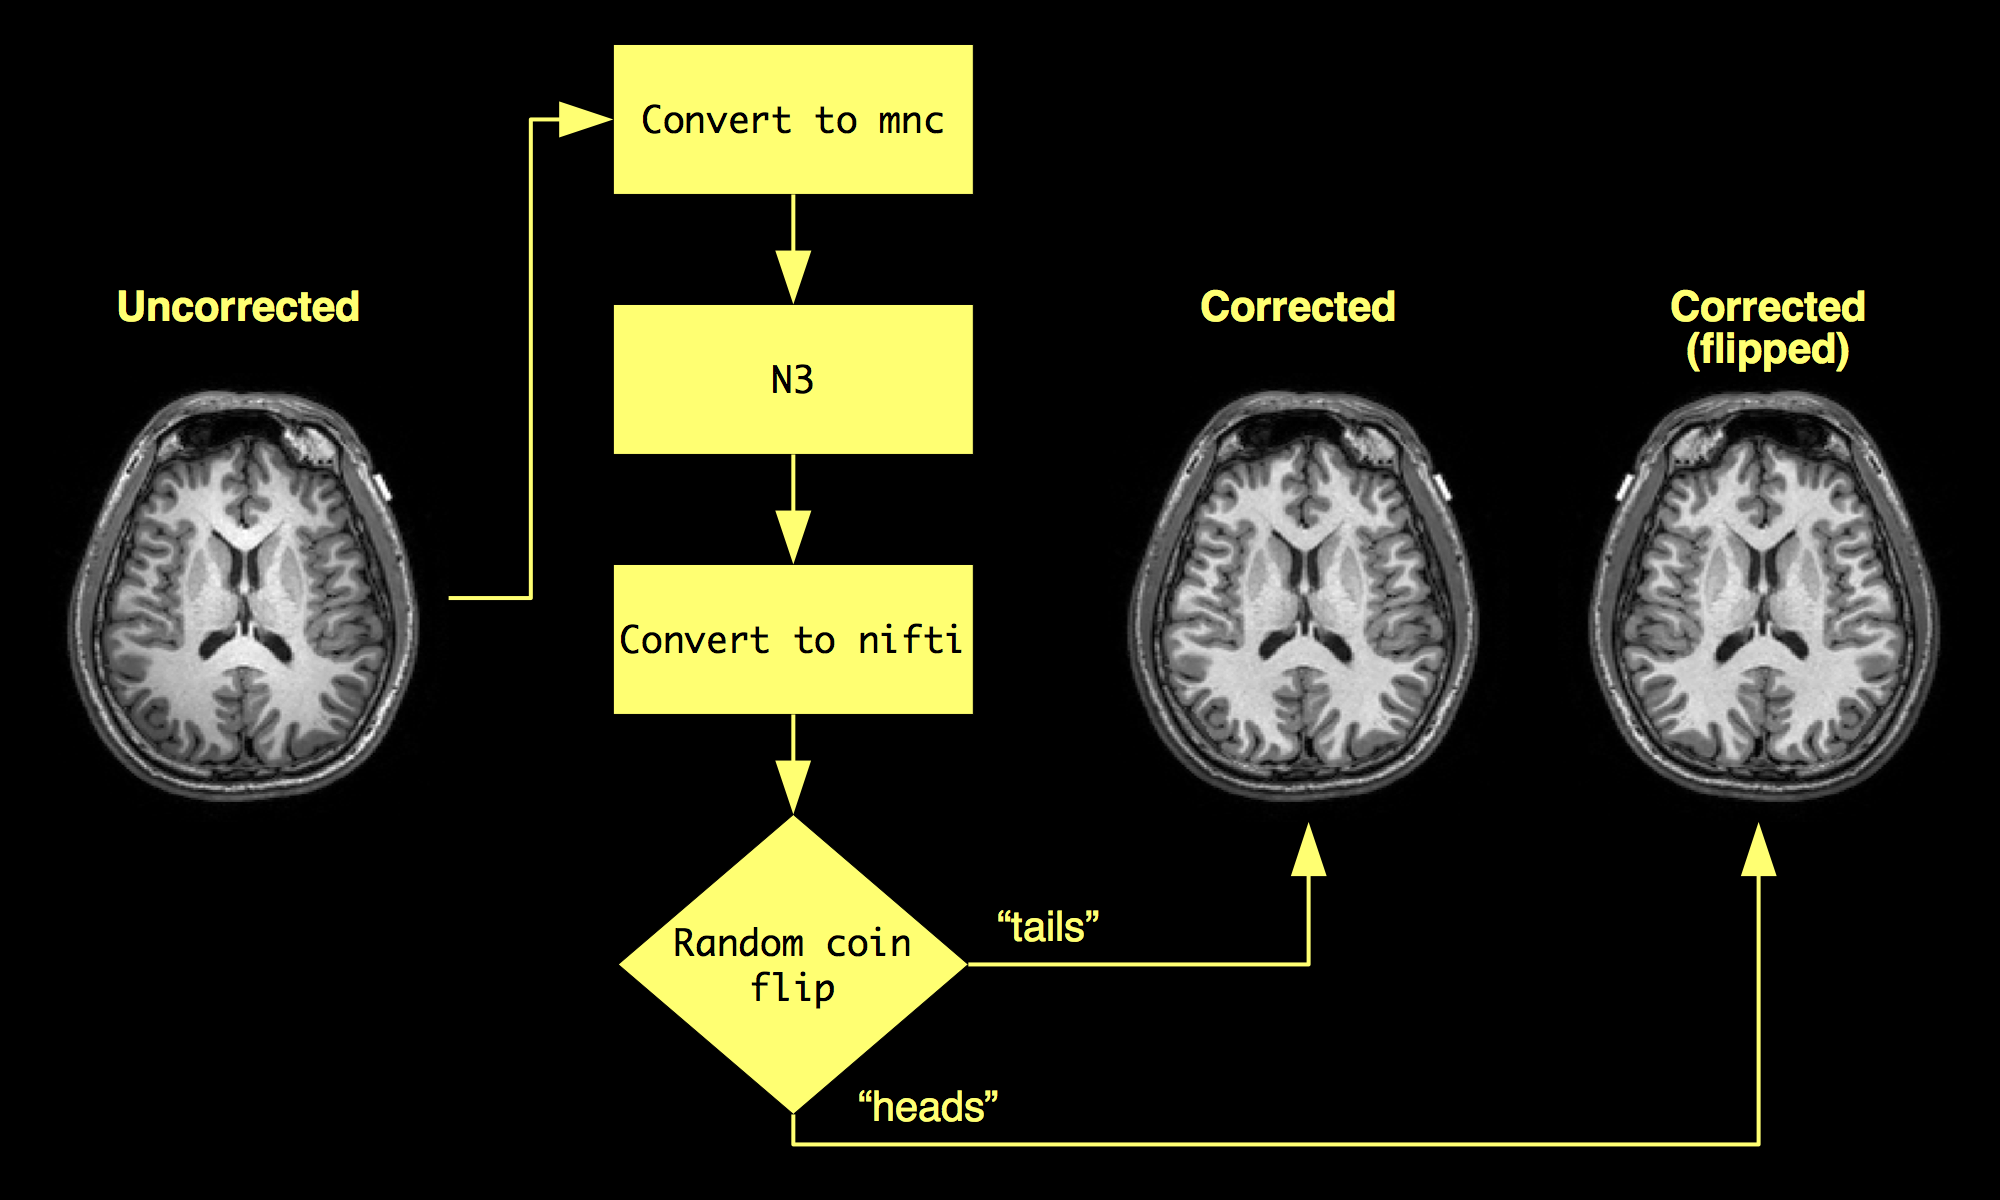
\includegraphics{./tools/n4/figures/whyN4.png}

\end{frame}

\begin{frame}[fragile]{\texttt{N4BiasFieldCorrection}}

\begin{Shaded}
\begin{Highlighting}[]
\NormalTok{$ }\KeywordTok{N4BiasFieldCorrection} \NormalTok{--help}

\KeywordTok{COMMAND}\NormalTok{:}
     \KeywordTok{N4BiasFieldCorrection}
          \KeywordTok{N4} \NormalTok{is a variant of the popular N3 (nonparameteric nonuniform normalization)}
          \KeywordTok{retrospective} \NormalTok{bias correction algorithm. Based on the assumption that the}
          \KeywordTok{corruption} \NormalTok{of the low frequency bias field can be modeled as a convolution of}
          \KeywordTok{the} \NormalTok{intensity histogram by a Gaussian, the basic algorithmic protocol is to}
          \KeywordTok{iterate} \NormalTok{between deconvolving the intensity histogram by a Gaussian, remapping}
          \KeywordTok{the} \NormalTok{intensities, and then spatially smoothing this result by a B-spline modeling}
          \KeywordTok{of} \NormalTok{the bias field itself. The modifications from and improvements obtained over}
          \KeywordTok{the} \NormalTok{original N3 algorithm are described in the following paper: N. Tustison et}
          \KeywordTok{al.}\NormalTok{, N4ITK: Improved N3 Bias Correction, IEEE Transactions on Medical Imaging,}
          \KeywordTok{29}\NormalTok{(6):}\KeywordTok{1310-1320}\NormalTok{, June 2010.}

\KeywordTok{OPTIONS}\NormalTok{:}
     \KeywordTok{-d}\NormalTok{, --image-dimensionality 2/3/4}
          \KeywordTok{This} \NormalTok{option forces the image to be treated as a specified-dimensional image. If}
          \KeywordTok{not} \NormalTok{specified, N4 tries to infer the dimensionality from the input image.}

     \KeywordTok{-i}\NormalTok{, --input-image inputImageFilename}
          \KeywordTok{A} \NormalTok{scalar image is expected as input for bias correction. Since N4 log transforms}
          \KeywordTok{the} \NormalTok{intensities, negative values or values close to zero should be processed}
          \KeywordTok{prior} \NormalTok{to correction.}

     \KeywordTok{-x}\NormalTok{, --mask-image maskImageFilename}
          \KeywordTok{If} \NormalTok{a mask image is specified, the final bias correction is only performed in the}
          \KeywordTok{mask} \NormalTok{region. If a weight image is not specified, only intensity values inside}
          \KeywordTok{the} \NormalTok{masked region are used during the execution of the algorithm. If a weight}
          \KeywordTok{image} \NormalTok{is specified, only the non-zero weights are used in the execution of the}
          \KeywordTok{algorithm} \NormalTok{although the mask region defines where bias correction is performed in}
          \KeywordTok{the} \NormalTok{final output. Otherwise bias correction occurs over the entire image domain.}
          \KeywordTok{See} \NormalTok{also the option description for the weight image.}

     \KeywordTok{-r}\NormalTok{, --rescale-intensities 0/(1)}
          \KeywordTok{At} \NormalTok{each iteration, a new intensity mapping is calculated and applied but there}
          \KeywordTok{is} \NormalTok{nothing which constrains the new intensity range to be within certain values.}
          \KeywordTok{The} \NormalTok{result is that the range can }\StringTok{"drift"} \NormalTok{from the original at each iteration.}
          \KeywordTok{This} \NormalTok{option rescales to the [min,max] range of the original image intensities}
          \KeywordTok{within} \NormalTok{the user-specified mask.}

     \KeywordTok{-w}\NormalTok{, --weight-image weightImageFilename}
          \KeywordTok{The} \NormalTok{weight image allows the user to perform a relative weighting of specific}
          \KeywordTok{voxels} \NormalTok{during the B-spline fitting. For example, some studies have shown that N3}
          \KeywordTok{performed} \NormalTok{on white matter segmentations improves performance. If one has a}
          \KeywordTok{spatial} \NormalTok{probability map of the white matter, one can use this map to weight the}
          \KeywordTok{b-spline} \NormalTok{fitting towards those voxels which are more probabilistically}
          \KeywordTok{classified} \NormalTok{as white matter. See also the option description for the mask image.}

     \KeywordTok{-s}\NormalTok{, --shrink-factor 1/2/3/4/...}
          \KeywordTok{Running} \NormalTok{N4 on large images can be time consuming. To lessen computation time,}
          \KeywordTok{the} \NormalTok{input image can be resampled. The shrink factor, specified as a single}
          \KeywordTok{integer}\NormalTok{, describes this resampling. Shrink factors }\KeywordTok{<}\NormalTok{= 4 are commonly used.}

     \KeywordTok{-c}\NormalTok{, --convergence [}\KeywordTok{<}\NormalTok{numberOfIterations=50x50x50x}\KeywordTok{50>}\NormalTok{,}\KeywordTok{<}\NormalTok{convergenceThreshold=0.}\KeywordTok{0>}\NormalTok{]}
          \KeywordTok{Convergence} \NormalTok{is determined by calculating the coefficient of variation between}
          \KeywordTok{subsequent} \NormalTok{iterations. When this value is less than the specified threshold from}
          \KeywordTok{the} \NormalTok{previous iteration or the maximum number of iterations is exceeded the}
          \KeywordTok{program} \NormalTok{terminates. Multiple resolutions can be specified by using }\StringTok{'x'} \NormalTok{between}
          \KeywordTok{the} \NormalTok{number of iterations at each resolution, e.g. 100x50x50.}

     \KeywordTok{-b}\NormalTok{, --bspline-fitting [splineDistance,}\KeywordTok{<}\NormalTok{splineOrder=}\KeywordTok{3>}\NormalTok{]}
                           \NormalTok{[}\KeywordTok{initialMeshResolution}\NormalTok{,}\KeywordTok{<}\NormalTok{splineOrder=}\KeywordTok{3>}\NormalTok{]}
          \KeywordTok{These} \NormalTok{options describe the b-spline fitting parameters. The initial b-spline}
          \KeywordTok{mesh} \NormalTok{at the coarsest resolution is specified either as the number of elements in}
          \KeywordTok{each} \NormalTok{dimension, e.g. 2x2x3 for 3-D images, or it can be specified as a single}
          \KeywordTok{scalar} \NormalTok{parameter which describes the isotropic sizing of the mesh elements. The}
          \KeywordTok{latter} \NormalTok{option is typically preferred. For each subsequent level, the spline}
          \KeywordTok{distance} \NormalTok{decreases in half, or equivalently, the number of mesh elements doubles}
          \KeywordTok{Cubic} \NormalTok{splines (order = 3) }\KeywordTok{are} \NormalTok{typically used.}

     \KeywordTok{-t}\NormalTok{, --histogram-sharpening [}\KeywordTok{<}\NormalTok{FWHM=0.}\KeywordTok{15>}\NormalTok{,}\KeywordTok{<}\NormalTok{wienerNoise=0.}\KeywordTok{01>}\NormalTok{,}\KeywordTok{<}\NormalTok{numberOfHistogramBins=}\KeywordTok{200>}\NormalTok{]}
          \KeywordTok{These} \NormalTok{options describe the histogram sharpening parameters, i.e. the}
          \KeywordTok{deconvolution} \NormalTok{step parameters described in the original N3 algorithm. The}
          \KeywordTok{default} \NormalTok{values have been shown to work fairly well.}

     \KeywordTok{-o}\NormalTok{, --output correctedImage}
                  \NormalTok{[}\KeywordTok{correctedImage}\NormalTok{,}\KeywordTok{<}\NormalTok{biasField}\KeywordTok{>}\NormalTok{]}
          \KeywordTok{The} \NormalTok{output consists of the bias corrected version of the input image.}
          \KeywordTok{Optionally}\NormalTok{, one can also output the estimated bias field.}

     \KeywordTok{--version}
          \KeywordTok{Get} \NormalTok{Version Information.}

     \KeywordTok{-v}\NormalTok{, --verbose (0)}\KeywordTok{/1}
          \KeywordTok{Verbose} \NormalTok{output.}

     \KeywordTok{-h}
          \KeywordTok{Print} \NormalTok{the help menu (short version)}\KeywordTok{.}

     \KeywordTok{--help}
          \KeywordTok{Print} \NormalTok{the help menu.}
          \KeywordTok{<VALUES>}\NormalTok{: 1}
\end{Highlighting}
\end{Shaded}

\textless{}-- \#\# Atropos -- cutting the threads of fate

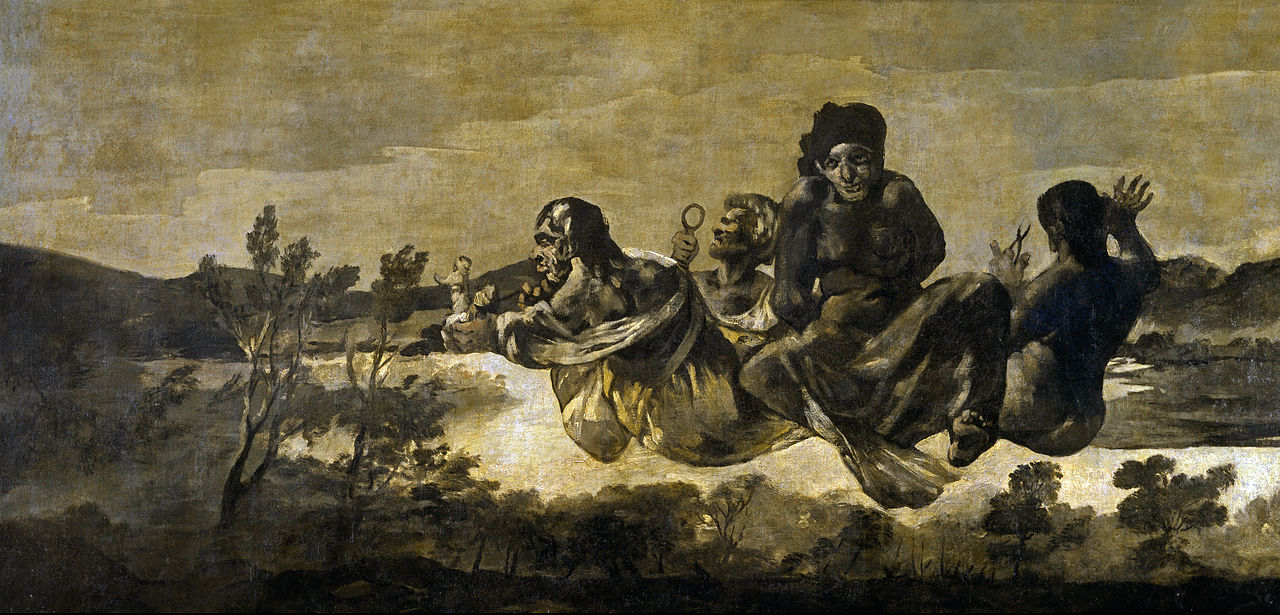
\includegraphics{./papers/figures/Atropos_deGoya.jpg} --\textgreater{}

\end{frame}

\begin{frame}{Atropos: flexible code base}

``20+ years of development. \emph{Show me the code!}''

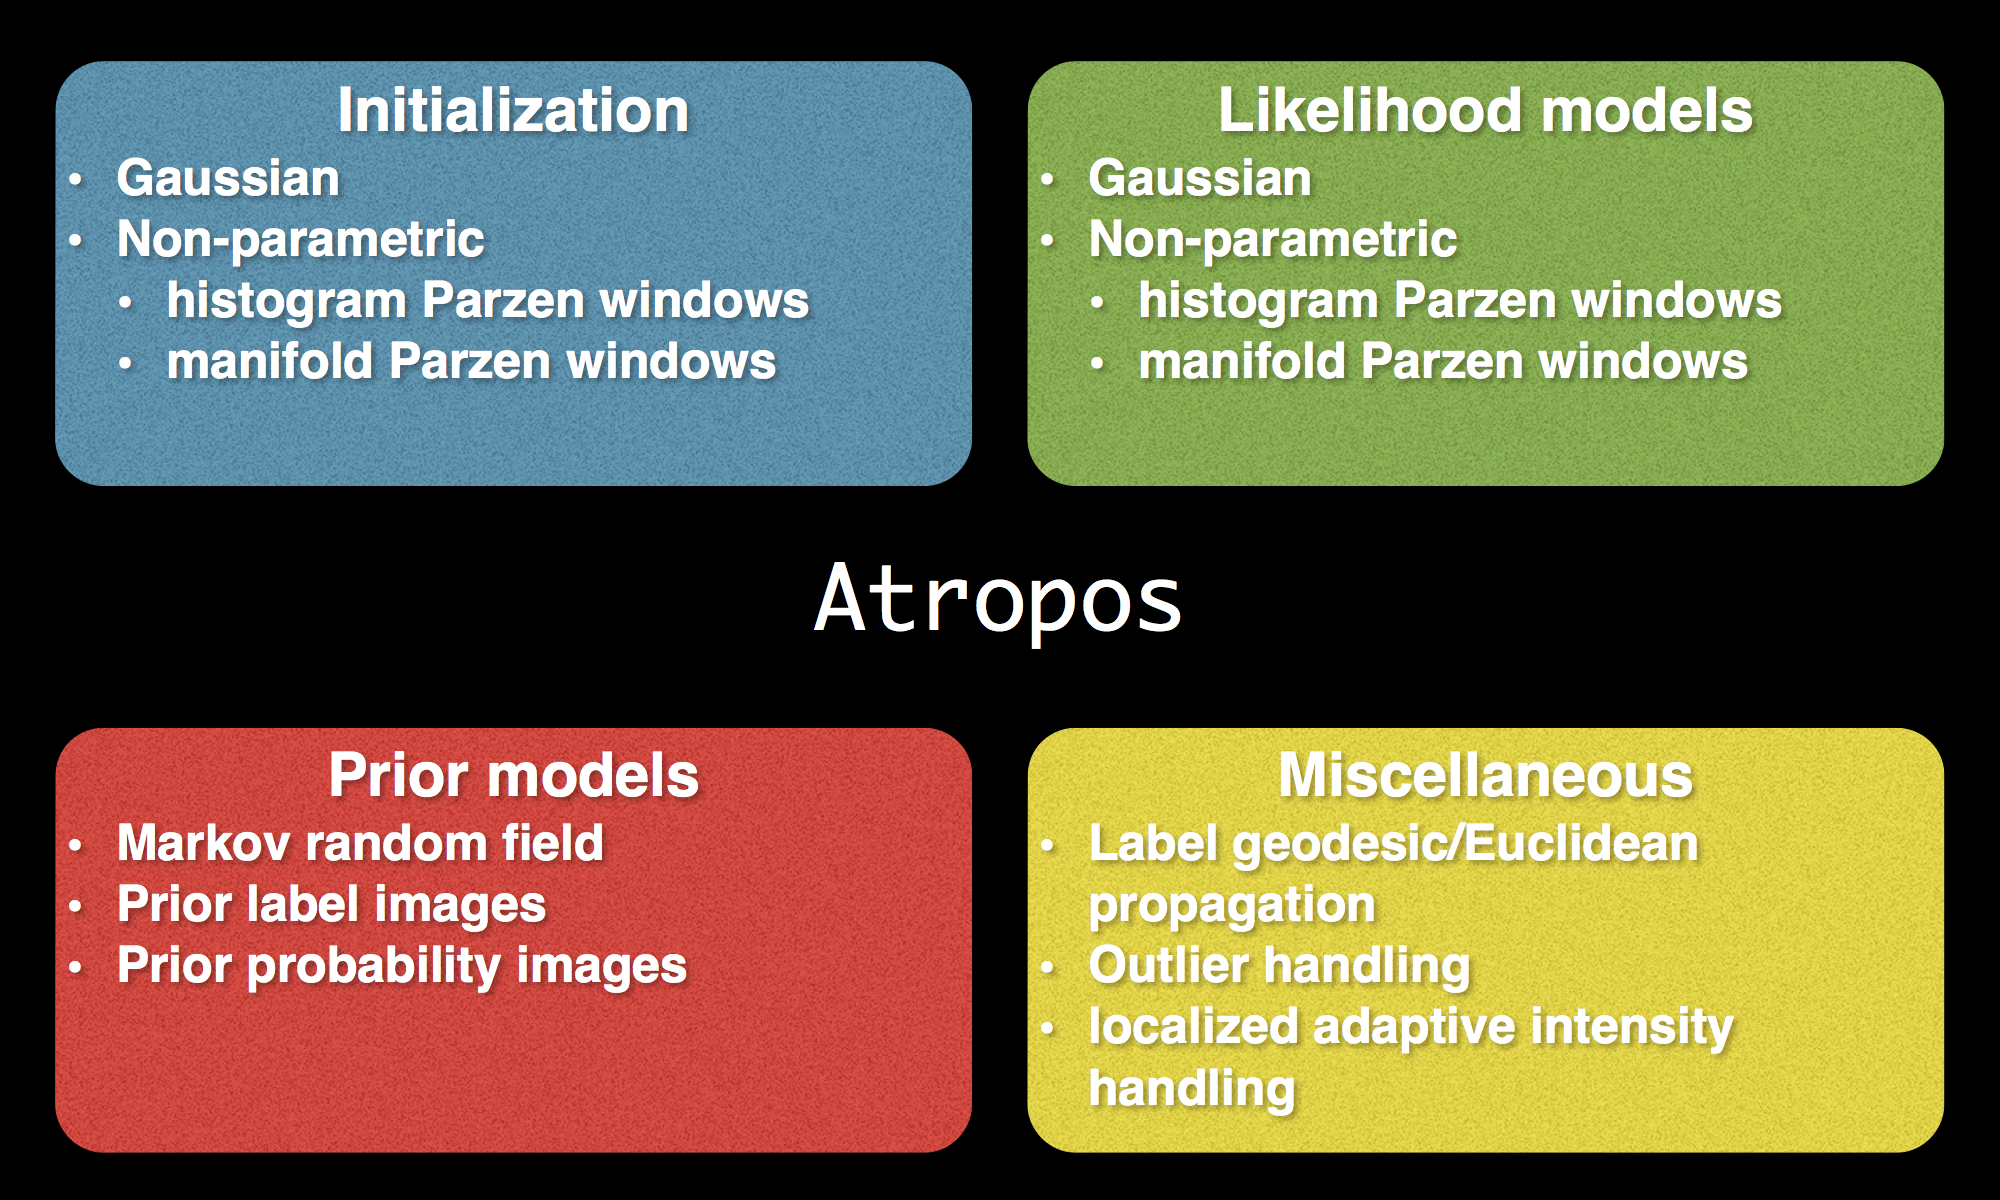
\includegraphics{./tools/atropos/figures/atropos.png}

\end{frame}

\begin{frame}[fragile]{\texttt{Atropos}}

\begin{Shaded}
\begin{Highlighting}[]
\NormalTok{$ }\KeywordTok{Atropos} \NormalTok{--help}

\KeywordTok{COMMAND}\NormalTok{:}
     \KeywordTok{Atropos}
          \KeywordTok{A} \NormalTok{finite mixture modeling (FMM) }\KeywordTok{segmentation} \NormalTok{approach with possibilities for}
          \KeywordTok{specifying} \NormalTok{prior constraints. These prior constraints include the specification}
          \KeywordTok{of} \NormalTok{a prior label image, prior probability images (one for each class), }\KeywordTok{and/or} \NormalTok{an}
          \KeywordTok{MRF} \NormalTok{prior to enforce spatial smoothing of the labels. Similar algorithms include}
          \KeywordTok{FAST} \NormalTok{and SPM. Reference: Avants BB, Tustison NJ, Wu J, Cook PA, Gee JC. An open}
          \KeywordTok{source} \NormalTok{multivariate framework for n-tissue segmentation with evaluation on}
          \KeywordTok{public} \NormalTok{data. Neuroinformatics. 2011 Dec}\KeywordTok{;9}\NormalTok{(4):}\KeywordTok{381-400.}

\KeywordTok{OPTIONS}\NormalTok{:}
     \KeywordTok{-d}\NormalTok{, --image-dimensionality 2/3/4}
          \KeywordTok{This} \NormalTok{option forces the image to be treated as a specified-dimensional image. If}
          \KeywordTok{not} \NormalTok{specified, Atropos tries to infer the dimensionality from the first input}
          \KeywordTok{image.}

     \KeywordTok{-a}\NormalTok{, --intensity-image [intensityImage,}\KeywordTok{<}\NormalTok{adaptiveSmoothingWeight}\KeywordTok{>}\NormalTok{]}
          \KeywordTok{One} \NormalTok{or more scalar images is specified for segmentation using the}
          \KeywordTok{-a/--intensity-image} \NormalTok{option. For segmentation scenarios with no prior}
          \KeywordTok{information}\NormalTok{, the first scalar image encountered on the command line is used to}
          \KeywordTok{order} \NormalTok{labelings such that the class with the smallest intensity signature is}
          \KeywordTok{class} \StringTok{'1'} \NormalTok{through class }\StringTok{'N'} \NormalTok{which represents the voxels with the largest}
          \KeywordTok{intensity} \NormalTok{values. The optional adaptive smoothing weight parameter is applicable}
          \KeywordTok{only} \NormalTok{when using prior label or probability images. This scalar parameter is to}
          \KeywordTok{be} \NormalTok{specified between [0,1] which smooths each labeled region separately and}
          \KeywordTok{modulates} \NormalTok{the intensity measurement at each voxel in each intensity image}
          \KeywordTok{between} \NormalTok{the original intensity and its smoothed counterpart. The smoothness}
          \KeywordTok{parameters} \NormalTok{are governed by the -b/--bspline option.}

     \KeywordTok{-b}\NormalTok{, --bspline [}\KeywordTok{<}\NormalTok{numberOfLevels=}\KeywordTok{6>}\NormalTok{,}\KeywordTok{<}\NormalTok{initialMeshResolution=1x1x...}\KeywordTok{>}\NormalTok{,}\KeywordTok{<}\NormalTok{splineOrder=}\KeywordTok{3>}\NormalTok{]}
          \KeywordTok{If} \NormalTok{the adaptive smoothing weights are }\KeywordTok{>} \NormalTok{0, the intensity images are smoothed in}
          \KeywordTok{calculating} \NormalTok{the likelihood values. This is to account for subtle intensity}
          \KeywordTok{differences} \NormalTok{across the same tissue regions.}

     \KeywordTok{-i}\NormalTok{, --initialization Random[numberOfClasses]}
                          \KeywordTok{Otsu}\NormalTok{[numberOfTissueClasses]}
                          \KeywordTok{KMeans}\NormalTok{[numberOfTissueClasses,}\KeywordTok{<}\NormalTok{clusterCenters(in ascending order and for first intensity image only)}\KeywordTok{>}\NormalTok{]}
                          \KeywordTok{PriorProbabilityImages}\NormalTok{[numberOfTissueClasses,fileSeriesFormat(index=1 to numberOfClasses) }\KeywordTok{or} \NormalTok{vectorImage,priorWeighting,}\KeywordTok{<}\NormalTok{priorProbabilityThreshold}\KeywordTok{>}\NormalTok{]}
                          \KeywordTok{PriorLabelImage}\NormalTok{[numberOfTissueClasses,labelImage,priorWeighting]}
          \KeywordTok{To} \NormalTok{initialize the FMM parameters, one of the following options must be}
          \KeywordTok{specified.} \NormalTok{If one does not have prior label or probability images we recommend}
          \KeywordTok{using} \NormalTok{kmeans as it is typically faster than otsu and can be used with}
          \KeywordTok{multivariate} \NormalTok{initialization. However, since a Euclidean distance on the inter}
          \KeywordTok{cluster} \NormalTok{distances is used, one might have to appropriately scale the additional}
          \KeywordTok{input} \NormalTok{images. Random initialization is meant purely for intellectual curiosity.}
          \KeywordTok{The} \NormalTok{prior weighting (specified in the range [0,1]) }\KeywordTok{is} \NormalTok{used to modulate the}
          \KeywordTok{calculation} \NormalTok{of the posterior probabilities between the likelihood*mrfprior and}
          \KeywordTok{the} \NormalTok{likelihood*mrfprior*prior. For specifying many prior probability images for}
          \KeywordTok{a} \NormalTok{multi-label segmentation, we offer a minimize usage option (see -m)}\KeywordTok{.} \KeywordTok{With} \NormalTok{that}
          \KeywordTok{option} \NormalTok{one can specify a prior probability threshold in which only those pixels}
          \KeywordTok{exceeding} \NormalTok{that threshold are stored in memory.}

     \KeywordTok{-s}\NormalTok{, --partial-volume-label-set label1xlabel2xlabel3}
          \KeywordTok{The} \NormalTok{partial volume estimation option allows one to modelmixtures of classes}
          \KeywordTok{within} \NormalTok{single voxels. Atropos currently allows the user to model two class}
          \KeywordTok{mixtures} \NormalTok{per partial volume class. The user specifies a set of class labels per}
          \KeywordTok{partial} \NormalTok{volume class requested. For example, suppose the user was performing a}
          \KeywordTok{classic} \NormalTok{3-tissue segmentation (csf, gm, wm) }\KeywordTok{using} \NormalTok{kmeans initialization. Suppose}
          \KeywordTok{the} \NormalTok{user also wanted to model the partial voluming effects between csf/gm and}
          \KeywordTok{gm/wm.} \NormalTok{The user would specify it using -i kmeans[3] and -s 1x2 -s 2x3. So, for}
          \KeywordTok{this} \NormalTok{example, there would be 3 tissue classes and 2 partial volume classes.}
          \KeywordTok{Optionally}\NormalTok{,the user can limit partial volume handling to mrf considerations only}
          \KeywordTok{whereby} \NormalTok{the output would only be the three tissues.}

     \KeywordTok{--use-partial-volume-likelihoods} \NormalTok{1/(0)}
                                      \KeywordTok{true}\NormalTok{/}\KeywordTok{(false)}
          \KeywordTok{The} \NormalTok{user can specify whether or not to use the partial volume likelihoods, in}
          \KeywordTok{which} \NormalTok{case the partial volume class is considered separate from the tissue}
          \KeywordTok{classes.} \NormalTok{Alternatively, one can use the MRF only to handle partial volume in}
          \KeywordTok{which} \NormalTok{case, partial volume voxels are not considered as separate classes.}

     \KeywordTok{-p}\NormalTok{, --posterior-formulation Socrates[}\KeywordTok{<}\NormalTok{useMixtureModelProportions=}\KeywordTok{1>}\NormalTok{,}\KeywordTok{<}\NormalTok{initialAnnealingTemperature=}\KeywordTok{1>}\NormalTok{,}\KeywordTok{<}\NormalTok{annealingRate=}\KeywordTok{1>}\NormalTok{,}\KeywordTok{<}\NormalTok{minimumTemperature=0.}\KeywordTok{1>}\NormalTok{]}
                                 \KeywordTok{Plato}\NormalTok{[}\KeywordTok{<}\NormalTok{useMixtureModelProportions=}\KeywordTok{1>}\NormalTok{,}\KeywordTok{<}\NormalTok{initialAnnealingTemperature=}\KeywordTok{1>}\NormalTok{,}\KeywordTok{<}\NormalTok{annealingRate=}\KeywordTok{1>}\NormalTok{,}\KeywordTok{<}\NormalTok{minimumTemperature=0.}\KeywordTok{1>}\NormalTok{]}
                                 \KeywordTok{Aristotle}\NormalTok{[}\KeywordTok{<}\NormalTok{useMixtureModelProportions=}\KeywordTok{1>}\NormalTok{,}\KeywordTok{<}\NormalTok{initialAnnealingTemperature=}\KeywordTok{1>}\NormalTok{,}\KeywordTok{<}\NormalTok{annealingRate=}\KeywordTok{1>}\NormalTok{,}\KeywordTok{<}\NormalTok{minimumTemperature=0.}\KeywordTok{1>}\NormalTok{]}
                                 \KeywordTok{Sigmoid}\NormalTok{[}\KeywordTok{<}\NormalTok{useMixtureModelProportions=}\KeywordTok{1>}\NormalTok{,}\KeywordTok{<}\NormalTok{initialAnnealingTemperature=}\KeywordTok{1>}\NormalTok{,}\KeywordTok{<}\NormalTok{annealingRate=}\KeywordTok{1>}\NormalTok{,}\KeywordTok{<}\NormalTok{minimumTemperature=0.}\KeywordTok{1>}\NormalTok{]]}
          \KeywordTok{Different} \NormalTok{posterior probability formulations are possible as are different}
          \KeywordTok{update} \NormalTok{options. To guarantee theoretical convergence properties, a proper}
          \KeywordTok{formulation} \NormalTok{of the well-known iterated conditional modes (ICM) }\KeywordTok{uses} \NormalTok{an}
          \KeywordTok{asynchronous} \NormalTok{update step modulated by a specified annealing temperature. If one}
          \KeywordTok{sets} \NormalTok{the AnnealingTemperature }\KeywordTok{>} \NormalTok{1 in the posterior formulation a traditional}
          \KeywordTok{code} \NormalTok{set for a proper ICM update will be created. Otherwise, a synchronous}
          \KeywordTok{update} \NormalTok{step will take place at each iteration. The annealing temperature, T,}
          \KeywordTok{converts} \NormalTok{the posteriorProbability to posteriorProbability^(1/T) }\KeywordTok{over} \NormalTok{the course}
          \KeywordTok{of} \NormalTok{optimization.}

     \KeywordTok{-x}\NormalTok{, --mask-image maskImageFilename}
          \KeywordTok{The} \NormalTok{image mask (which is required) }\KeywordTok{defines} \NormalTok{the region which is to be labeled by}
          \KeywordTok{the} \NormalTok{Atropos algorithm.}

     \KeywordTok{-c}\NormalTok{, --convergence numberOfIterations}
                       \NormalTok{[}\KeywordTok{<}\OtherTok{numberOfIterations=}\NormalTok{5}\KeywordTok{>}\NormalTok{,}\KeywordTok{<}\OtherTok{convergenceThreshold=}\NormalTok{0.001}\KeywordTok{>}\NormalTok{]}
          \KeywordTok{Convergence} \NormalTok{is determined by calculating the mean maximum posterior probability}
          \KeywordTok{over} \NormalTok{the region of interest at each iteration. When this value decreases or}
          \KeywordTok{increases} \NormalTok{less than the specified threshold from the previous iteration or the}
          \KeywordTok{maximum} \NormalTok{number of iterations is exceeded the program terminates.}

     \KeywordTok{-k}\NormalTok{, --likelihood-model Gaussian}
                            \KeywordTok{HistogramParzenWindows}\NormalTok{[}\KeywordTok{<}\NormalTok{sigma=1.}\KeywordTok{0>}\NormalTok{,}\KeywordTok{<}\NormalTok{numberOfBins=}\KeywordTok{32>}\NormalTok{]}
                            \KeywordTok{ManifoldParzenWindows}\NormalTok{[}\KeywordTok{<}\NormalTok{pointSetSigma=1.}\KeywordTok{0>}\NormalTok{,}\KeywordTok{<}\NormalTok{evaluationKNeighborhood=}\KeywordTok{50>}\NormalTok{,}\KeywordTok{<}\NormalTok{CovarianceKNeighborhood=}\KeywordTok{0>}\NormalTok{,}\KeywordTok{<}\NormalTok{kernelSigma=}\KeywordTok{0>}\NormalTok{]}
                            \KeywordTok{JointShapeAndOrientationProbability}\NormalTok{[}\KeywordTok{<}\NormalTok{shapeSigma=1.}\KeywordTok{0>}\NormalTok{,}\KeywordTok{<}\NormalTok{numberOfShapeBins=}\KeywordTok{64>}\NormalTok{, }\KeywordTok{<}\NormalTok{orientationSigma=1.}\KeywordTok{0>}\NormalTok{, }\KeywordTok{<}\NormalTok{numberOfOrientationBins=}\KeywordTok{32>}\NormalTok{]}
                            \KeywordTok{LogEuclideanGaussian}
          \KeywordTok{Both} \NormalTok{parametric and non-parametric options exist in Atropos. The Gaussian}
          \KeywordTok{parametric} \NormalTok{option is commonly used (e.g. SPM }\KeywordTok{&} \KeywordTok{FAST}\NormalTok{) }\KeywordTok{where} \NormalTok{the mean and standard}
          \KeywordTok{deviation} \NormalTok{for the Gaussian of each class is calculated at each iteration. Other}
          \KeywordTok{groups} \NormalTok{use non-parametric approaches exemplified by option 2. We recommend using}
          \KeywordTok{options} \NormalTok{1 or 2 as they are fairly standard and the default parameters work}
          \KeywordTok{adequately.}

     \KeywordTok{-m}\NormalTok{, --mrf [}\KeywordTok{<}\NormalTok{smoothingFactor=0.}\KeywordTok{3>}\NormalTok{,}\KeywordTok{<}\NormalTok{radius=1x1x...}\KeywordTok{>}\NormalTok{]}
               \NormalTok{[}\KeywordTok{<mrfCoefficientImage>}\NormalTok{,}\KeywordTok{<}\NormalTok{radius=1x1x...}\KeywordTok{>}\NormalTok{]}
          \KeywordTok{Markov} \NormalTok{random field (MRF) }\KeywordTok{theory} \NormalTok{provides a general framework for enforcing}
          \KeywordTok{spatially} \NormalTok{contextual constraints on the segmentation solution. The default}
          \KeywordTok{smoothing} \NormalTok{factor of 0.3 provides a moderate amount of smoothing. Increasing this}
          \KeywordTok{number} \NormalTok{causes more smoothing whereas decreasing the number lessens the}
          \KeywordTok{smoothing.} \NormalTok{The radius parameter specifies the mrf neighborhood. Different update}
          \KeywordTok{schemes} \NormalTok{are possible but only the asynchronous updating has theoretical}
          \KeywordTok{convergence} \NormalTok{properties.}

     \KeywordTok{-g}\NormalTok{, --icm [}\KeywordTok{<}\NormalTok{useAsynchronousUpdate=}\KeywordTok{1>}\NormalTok{,}\KeywordTok{<}\NormalTok{maximumNumberOfICMIterations=}\KeywordTok{1>}\NormalTok{,}\KeywordTok{<}\NormalTok{icmCodeImage=}\StringTok{''}\KeywordTok{>}\NormalTok{]}
          \KeywordTok{Asynchronous} \NormalTok{updating requires the construction of an ICM code image which is a}
          \KeywordTok{label} \NormalTok{image (with labels in the range }\DataTypeTok{\{1,..,MaximumICMCode\}}\NormalTok{) }\KeywordTok{constructed} \NormalTok{such}
          \KeywordTok{that} \NormalTok{no MRF neighborhood has duplicate ICM code labels. Thus, to update the}
          \KeywordTok{voxel} \NormalTok{class labels we iterate through the code labels and, for each code label,}
          \KeywordTok{we} \NormalTok{iterate through the image and update the voxel class label that has the}
          \KeywordTok{corresponding} \NormalTok{ICM code label. One can print out the ICM code image by specifying}
          \KeywordTok{an} \NormalTok{ITK-compatible image filename.}

     \KeywordTok{-r}\NormalTok{, --use-random-seed 0/(1)}
          \KeywordTok{Initialize} \NormalTok{internal random number generator with a random seed. Otherwise,}
          \KeywordTok{initialize} \NormalTok{with a constant seed number.}

     \KeywordTok{-o}\NormalTok{, --output [classifiedImage,}\KeywordTok{<}\NormalTok{posteriorProbabilityImageFileNameFormat}\KeywordTok{>}\NormalTok{]}
          \KeywordTok{The} \NormalTok{output consists of a labeled image where each voxel in the masked region is}
          \KeywordTok{assigned} \NormalTok{a label from 1, 2, ..., N. Optionally, one can also output the}
          \KeywordTok{posterior} \NormalTok{probability images specified in the same format as the prior}
          \KeywordTok{probability} \NormalTok{images, e.g. posterior%02d.nii.gz (C-style file name formatting)}\KeywordTok{.}

     \KeywordTok{-u}\NormalTok{, --minimize-memory-usage (0)}\KeywordTok{/1}
          \KeywordTok{By} \NormalTok{default, memory usage is not minimized, however, if this is needed, the}
          \KeywordTok{various} \NormalTok{probability and distance images are calculated on the fly instead of}
          \KeywordTok{being} \NormalTok{stored in memory at each iteration. Also, if prior probability images are}
          \KeywordTok{used}\NormalTok{, only the non-negligible pixel values are stored in memory.}
          \KeywordTok{<VALUES>}\NormalTok{: 0}

     \KeywordTok{-w}\NormalTok{, --winsorize-outliers BoxPlot[}\KeywordTok{<}\NormalTok{lowerPercentile=0.}\KeywordTok{25>}\NormalTok{,}\KeywordTok{<}\NormalTok{upperPercentile=0.}\KeywordTok{75>}\NormalTok{,}\KeywordTok{<}\NormalTok{whiskerLength=1.}\KeywordTok{5>}\NormalTok{]}
                              \KeywordTok{GrubbsRosner}\NormalTok{[}\KeywordTok{<}\NormalTok{significanceLevel=0.}\KeywordTok{05>}\NormalTok{,}\KeywordTok{<}\NormalTok{winsorizingLevel=0.}\KeywordTok{10>}\NormalTok{]}
          \KeywordTok{To} \NormalTok{remove the effects of outliers in calculating the weighted mean and weighted}
          \KeywordTok{covariance}\NormalTok{, the user can opt to remove the outliers through the options}
          \KeywordTok{specified} \NormalTok{below.}

     \KeywordTok{-e}\NormalTok{, --use-euclidean-distance (0)}\KeywordTok{/1}
          \KeywordTok{Given} \NormalTok{prior label or probability images, the labels are propagated throughout}
          \KeywordTok{the} \NormalTok{masked region so that every voxel in the mask is labeled. Propagation is}
          \KeywordTok{done} \KeywordTok{by} \NormalTok{using a signed distance transform of the label. Alternatively,}
          \KeywordTok{propagation} \NormalTok{of the labels with the fast marching filter respects the distance}
          \KeywordTok{along} \NormalTok{the shape of the mask (e.g. the sinuous sulci and gyri of the cortex.}
          \KeywordTok{<VALUES>}\NormalTok{: 0}

     \KeywordTok{-l}\NormalTok{, --label-propagation whichLabel[lambda=0.0,}\KeywordTok{<}\NormalTok{boundaryProbability=1.}\KeywordTok{0>}\NormalTok{]}
          \KeywordTok{The} \NormalTok{propagation of each prior label can be controlled by the lambda and boundary}
          \KeywordTok{probability} \NormalTok{parameters. The latter parameter is the probability (in the range}
          \NormalTok{[}\KeywordTok{0}\NormalTok{,1]) }\KeywordTok{of} \NormalTok{the label on the boundary which increases linearly to a maximum value}
          \KeywordTok{of} \NormalTok{1.0 in the interior of the labeled region. The former parameter dictates the}
          \KeywordTok{exponential} \NormalTok{decay of probability propagation outside the labeled region from the}
          \KeywordTok{boundary} \NormalTok{probability, i.e. boundaryProbability*exp( -lambda * distance )}\KeywordTok{.}

     \KeywordTok{-v}\NormalTok{, --verbose (0)}\KeywordTok{/1}
          \KeywordTok{Verbose} \NormalTok{output.}

     \KeywordTok{-h}
          \KeywordTok{Print} \NormalTok{the help menu (short version)}\KeywordTok{.}

     \KeywordTok{--help}
          \KeywordTok{Print} \NormalTok{the help menu.}
          \KeywordTok{<VALUES>}\NormalTok{: 1}
\end{Highlighting}
\end{Shaded}

\end{frame}

\begin{frame}[fragile]{\texttt{DenoiseImage} --- contribution from Jose
Manjon}

\begin{Shaded}
\begin{Highlighting}[]
\NormalTok{$ }\KeywordTok{DenoiseImage} \NormalTok{--help}


\KeywordTok{COMMAND}\NormalTok{:}
     \KeywordTok{DenoiseImage}
          \KeywordTok{Denoise} \NormalTok{an image using a spatially adaptive filter originally described in J. V.}
          \KeywordTok{Manjon}\NormalTok{, P. Coupe, Luis Marti-Bonmati, D. L. Collins, and M. Robles. Adaptive}
          \KeywordTok{Non-Local} \NormalTok{Means Denoising of MR Images With Spatially Varying Noise Levels,}
          \KeywordTok{Journal} \NormalTok{of Magnetic Resonance Imaging, 31:192-203, June 2010.}

\KeywordTok{OPTIONS}\NormalTok{:}
     \KeywordTok{-d}\NormalTok{, --image-dimensionality 2/3/4}
          \KeywordTok{This} \NormalTok{option forces the image to be treated as a specified-dimensional image. If}
          \KeywordTok{not} \NormalTok{specified, the program tries to infer the dimensionality from the input}
          \KeywordTok{image.}

     \KeywordTok{-i}\NormalTok{, --input-image inputImageFilename}
          \KeywordTok{A} \NormalTok{scalar image is expected as input for noise correction.}

     \KeywordTok{-n}\NormalTok{, --noise-model Rician/(Gaussian)}
          \KeywordTok{Employ} \NormalTok{a Rician or Gaussian noise model.}

     \KeywordTok{-x}\NormalTok{, --mask-image maskImageFilename}
          \KeywordTok{If} \NormalTok{a mask image is specified, denoising is only performed in the mask region.}

     \KeywordTok{-s}\NormalTok{, --shrink-factor (1)}\KeywordTok{/2/3/...}
          \KeywordTok{Running} \NormalTok{noise correction on large images can be time consuming. To lessen}
          \KeywordTok{computation} \NormalTok{time, the input image can be resampled. The shrink factor, specified}
          \KeywordTok{as} \NormalTok{a single integer, describes this resampling. Shrink factor = 1 is the}
          \KeywordTok{default.}

     \KeywordTok{-p}\NormalTok{, --patch-radius 1}
                        \KeywordTok{1x1x1}
          \KeywordTok{Patch} \NormalTok{radius. Default = 1x1x1}

     \KeywordTok{-r}\NormalTok{, --search-radius 3}
                         \KeywordTok{3x3x3}
          \KeywordTok{Search} \NormalTok{radius. Default = 3x3x3.}

     \KeywordTok{-o}\NormalTok{, --output correctedImage}
                  \NormalTok{[}\KeywordTok{correctedImage}\NormalTok{,}\KeywordTok{<}\NormalTok{noiseImage}\KeywordTok{>}\NormalTok{]}
          \KeywordTok{The} \NormalTok{output consists of the noise corrected version of the input image.}
          \KeywordTok{Optionally}\NormalTok{, one can also output the estimated noise image.}

     \KeywordTok{--version}
          \KeywordTok{Get} \NormalTok{Version Information.}

     \KeywordTok{-v}\NormalTok{, --verbose (0)}\KeywordTok{/1}
          \KeywordTok{Verbose} \NormalTok{output.}

     \KeywordTok{-h}
          \KeywordTok{Print} \NormalTok{the help menu (short version)}\KeywordTok{.}

     \KeywordTok{--help}
          \KeywordTok{Print} \NormalTok{the help menu.}
          \KeywordTok{<VALUES>}\NormalTok{: 1}
\end{Highlighting}
\end{Shaded}

\end{frame}

\begin{frame}{Multi-atlas segmentation}

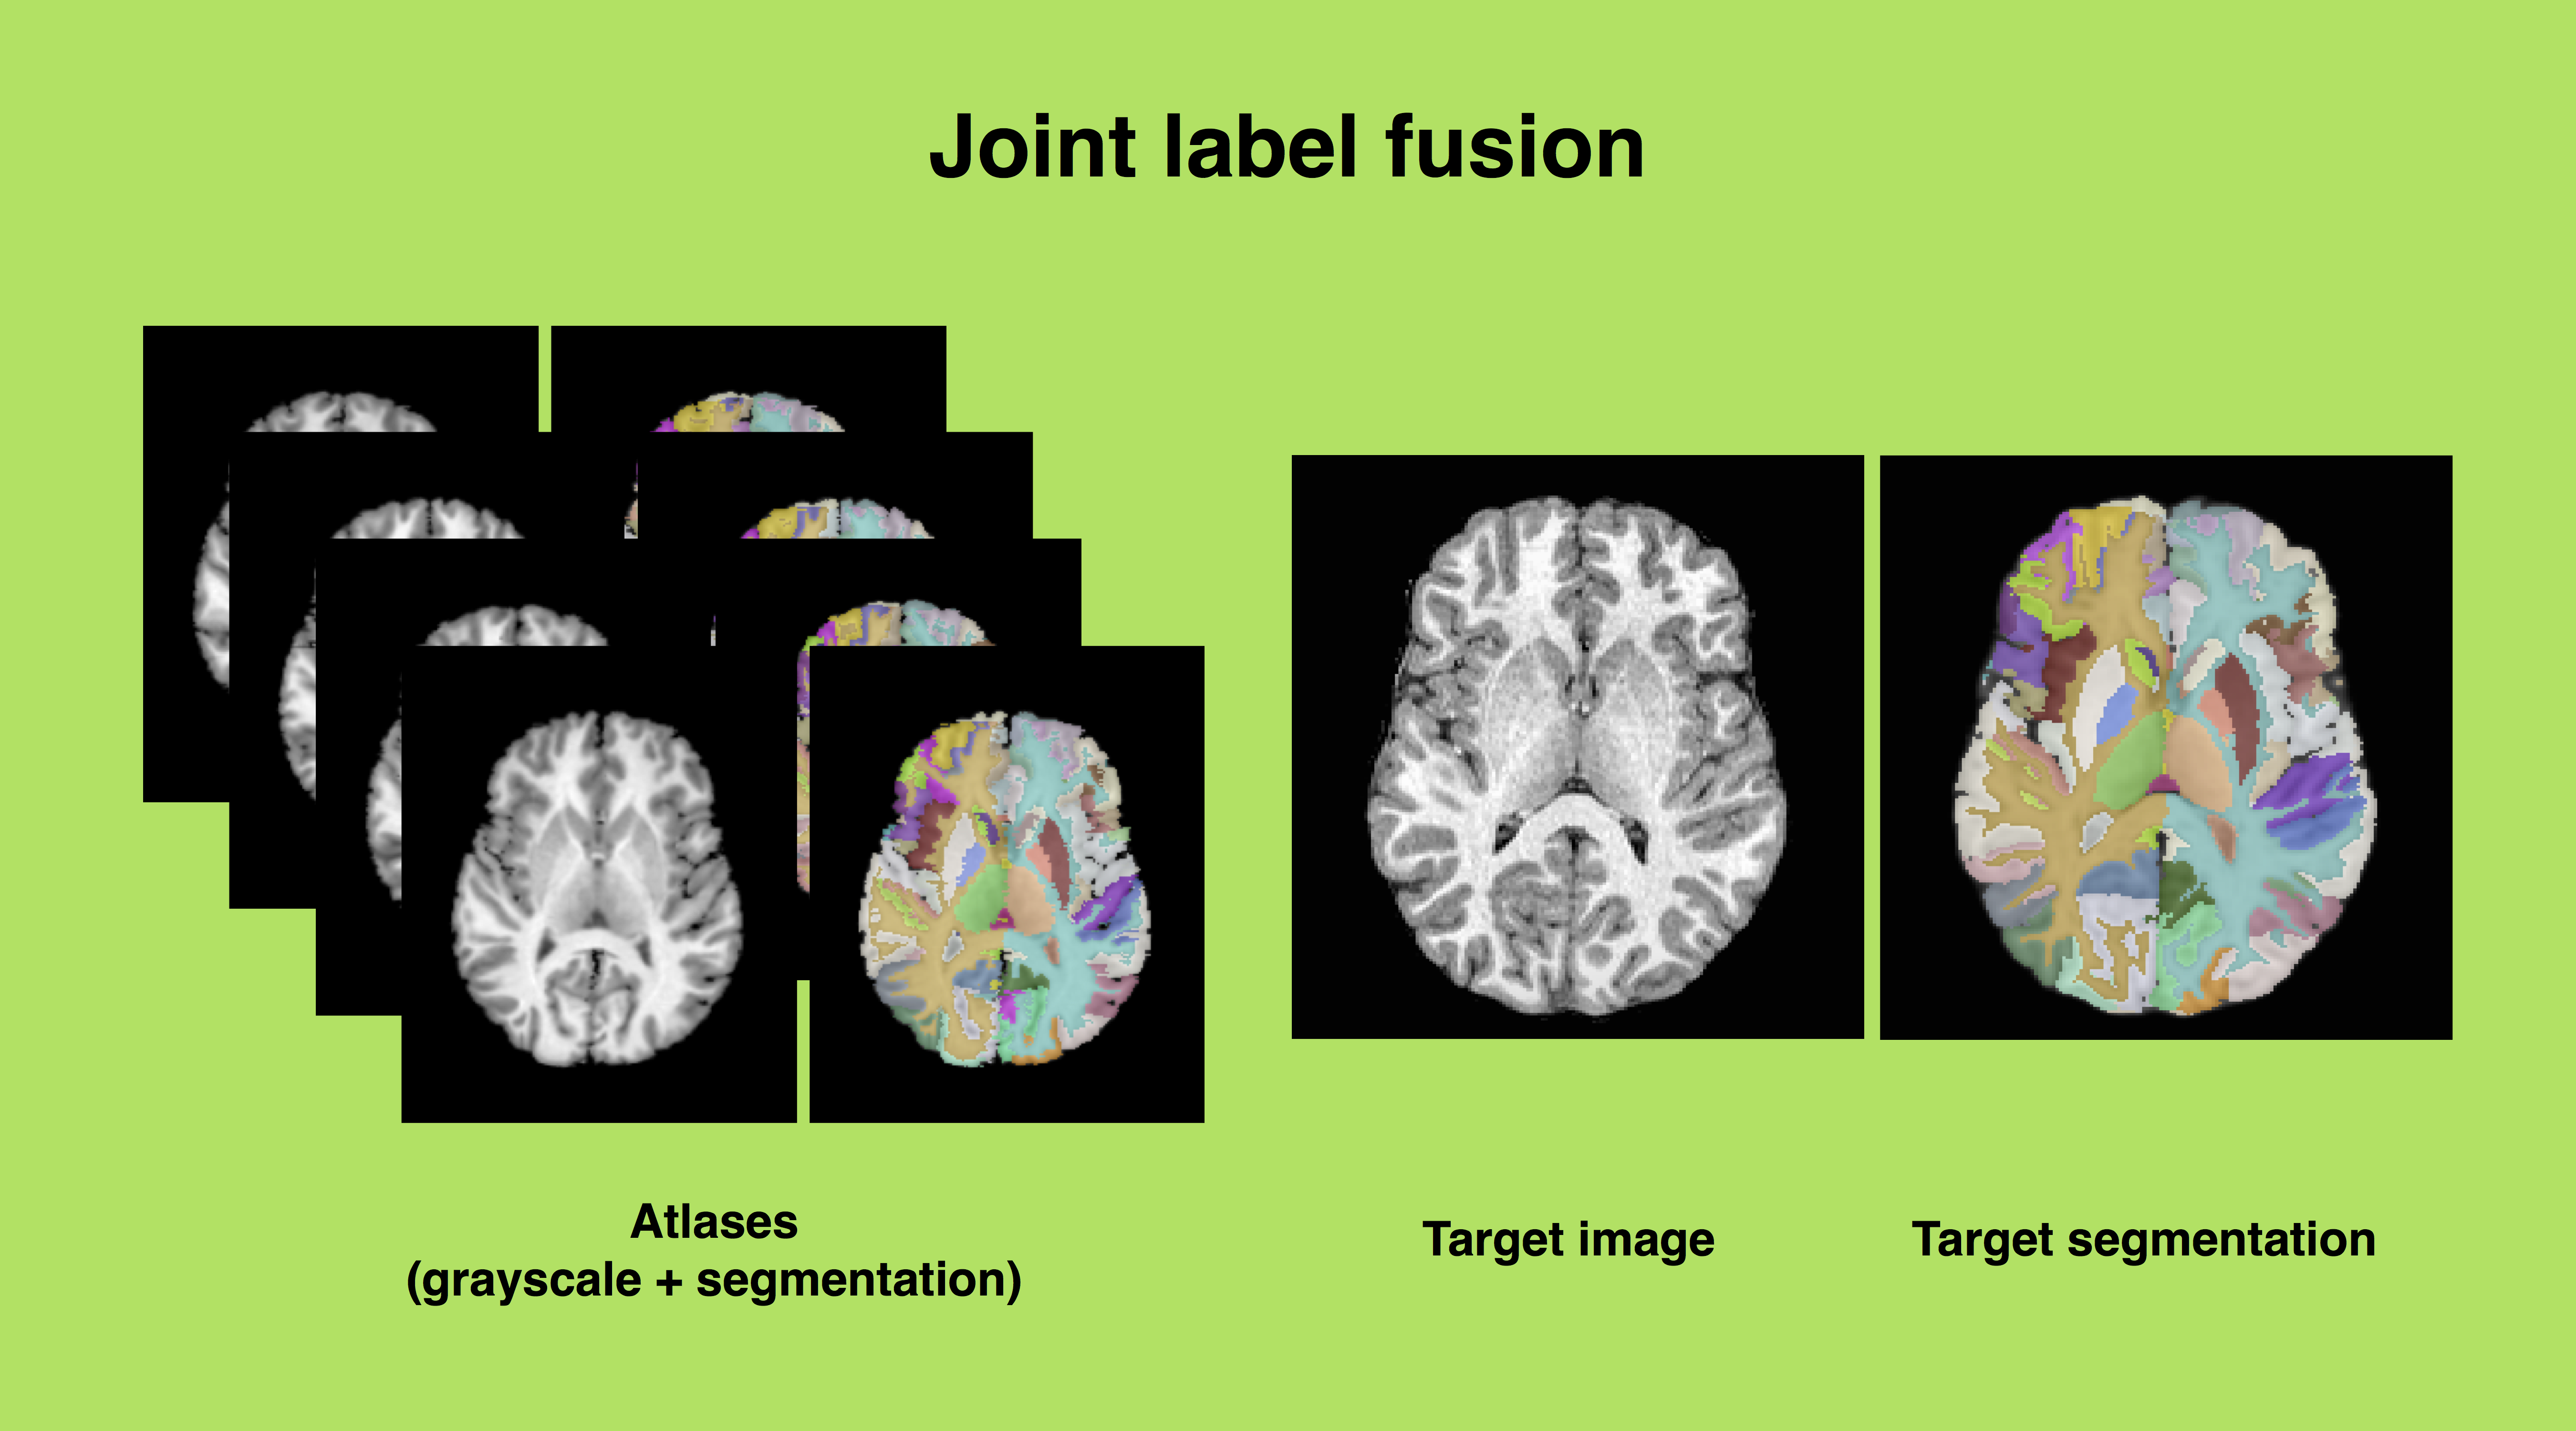
\includegraphics{./tools/jointfusion/figures/jointLabelFusion.png}

\end{frame}

\begin{frame}{New work: joint intensity fusion}

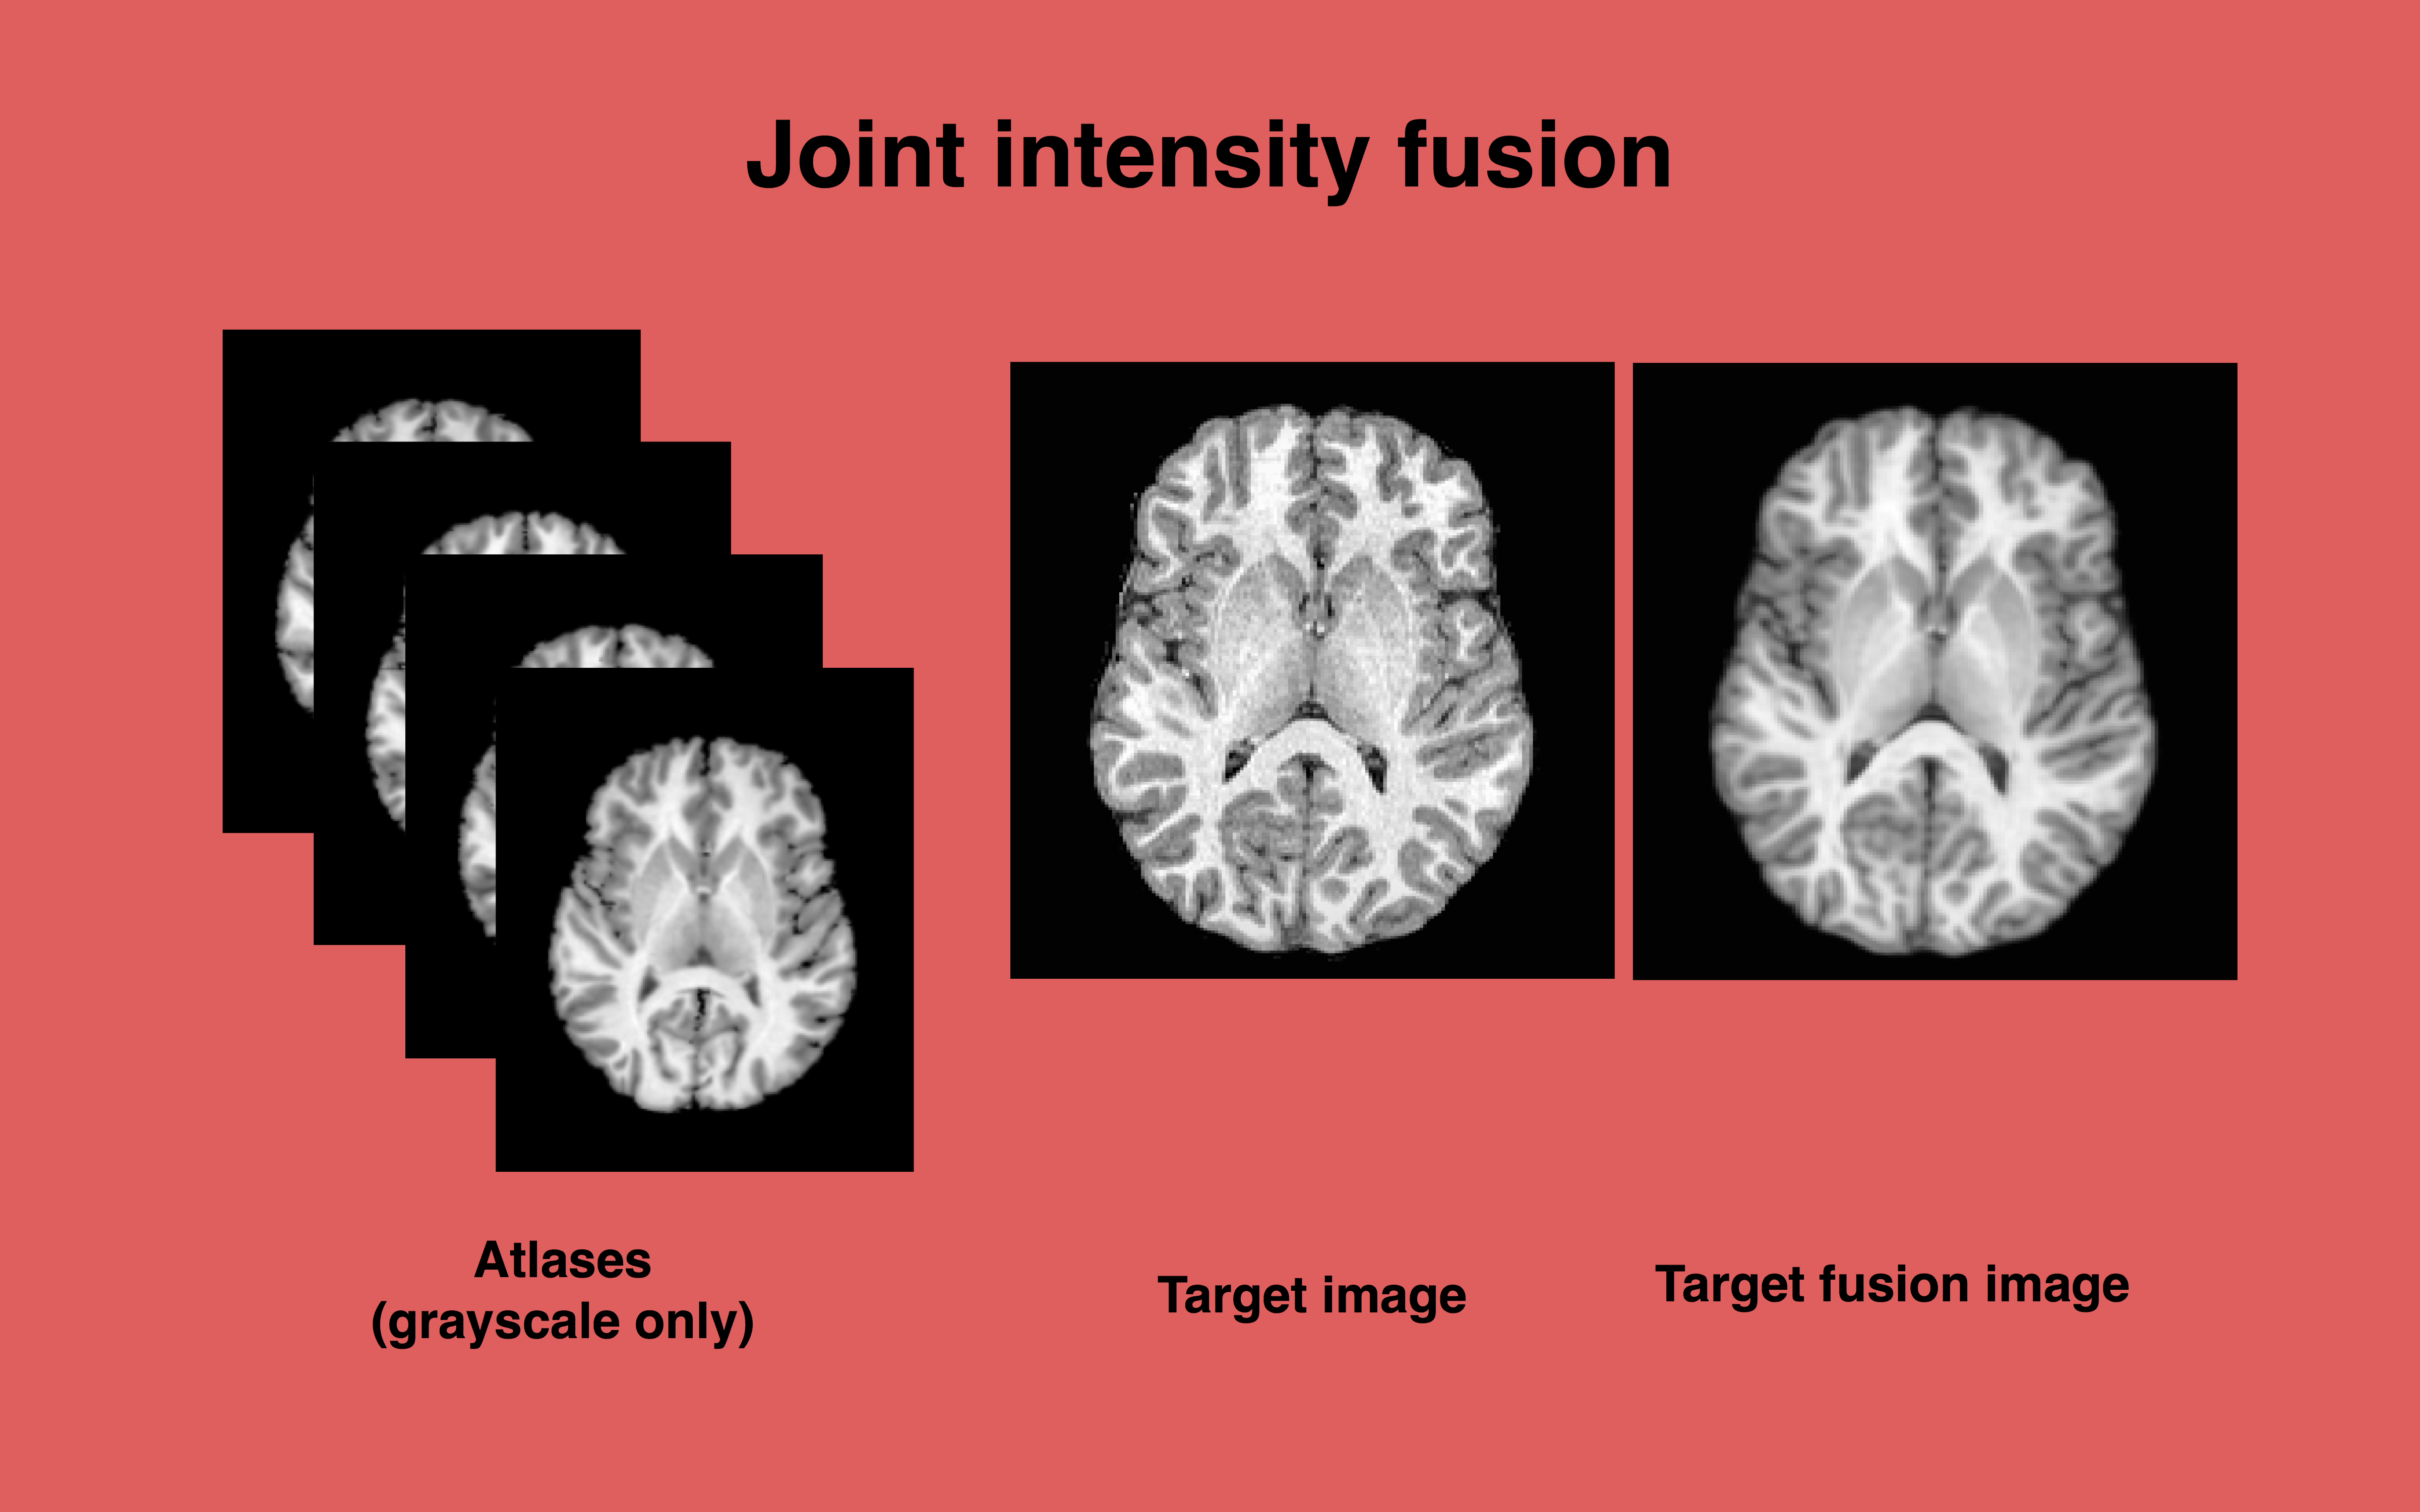
\includegraphics{./tools/jointfusion/figures/jointIntensityFusion.png}

\end{frame}

\begin{frame}{Possible uses}

\begin{itemize}
\item
  ``Correct'' images

  \begin{itemize}
  \item
    motion correction
  \item
    ``remove'' lesions
  \end{itemize}
\item
  Project atlas set intensity signature
\item
  Use in ``corrective learning''
\end{itemize}

\end{frame}

\begin{frame}[fragile]{\texttt{antsJointFusion} --- contribution from
Hongzhi Wang (with some added features)}

\begin{Shaded}
\begin{Highlighting}[]
\NormalTok{$ }\KeywordTok{antsJointFusion} \NormalTok{--help}

\KeywordTok{COMMAND}\NormalTok{:}
     \KeywordTok{antsJointFusion}
          \KeywordTok{antsJointFusion} \NormalTok{is an image fusion algorithm developed by Hongzhi Wang and Paul}
          \KeywordTok{Yushkevich} \NormalTok{which won segmentation challenges at MICCAI 2012 and MICCAI 2013. The}
          \KeywordTok{original} \NormalTok{label fusion framework was extended to accommodate intensities by Brian}
          \KeywordTok{Avants.} \NormalTok{This implementation is based on Paul}\StringTok{'s original ITK-style implementation}
\StringTok{          and Brian'}\NormalTok{s ANTsR implementation. References include 1) }\KeywordTok{H.} \NormalTok{Wang, J. W. Suh, S.}
          \KeywordTok{Das}\NormalTok{, J. Pluta, C. Craige, P. Yushkevich, Multi-atlas segmentation with joint}
          \KeywordTok{label} \NormalTok{fusion IEEE Trans. on Pattern Analysis and Machine Intelligence, 35(3),}
          \KeywordTok{611-623}\NormalTok{, 2013. and 2) }\KeywordTok{H.} \NormalTok{Wang and P. A. Yushkevich, Multi-atlas segmentation}
          \KeywordTok{with} \NormalTok{joint label fusion and corrective learning--an open source implementation,}
          \KeywordTok{Front.} \NormalTok{Neuroinform., 2013.}

\KeywordTok{OPTIONS}\NormalTok{:}
     \KeywordTok{-d}\NormalTok{, --image-dimensionality 2/3/4}
          \KeywordTok{This} \NormalTok{option forces the image to be treated as a specified-dimensional image. If}
          \KeywordTok{not} \NormalTok{specified, the program tries to infer the dimensionality from the input}
          \KeywordTok{image.}

     \KeywordTok{-t}\NormalTok{, --target-image targetImage}
                        \NormalTok{[}\KeywordTok{targetImageModality0}\NormalTok{,targetImageModality1,...,targetImageModalityN]}
          \KeywordTok{The} \NormalTok{target image (or multimodal target images) }\KeywordTok{assumed} \NormalTok{to be aligned to a common}
          \KeywordTok{image} \NormalTok{domain.}

     \KeywordTok{-g}\NormalTok{, --atlas-image atlasImage}
                       \NormalTok{[}\KeywordTok{atlasImageModality0}\NormalTok{,atlasImageModality1,...,atlasImageModalityN]}
          \KeywordTok{The} \NormalTok{atlas image (or multimodal atlas images) }\KeywordTok{assumed} \NormalTok{to be aligned to a common}
          \KeywordTok{image} \NormalTok{domain.}

     \KeywordTok{-l}\NormalTok{, --atlas-segmentation atlasSegmentation}
          \KeywordTok{The} \NormalTok{atlas segmentation images. For performing label fusion the number of}
          \KeywordTok{specified} \NormalTok{segmentations should be identical to the number of atlas image sets.}

     \KeywordTok{-a}\NormalTok{, --alpha 0.1}
          \KeywordTok{Regularization} \NormalTok{term added to matrix Mx for calculating the inverse. Default =}
          \KeywordTok{0.1}

     \KeywordTok{-b}\NormalTok{, --beta 2.0}
          \KeywordTok{Exponent} \NormalTok{for mapping intensity difference to the joint error. Default = 2.0}

     \KeywordTok{-r}\NormalTok{, --retain-label-posterior-images (0)}\KeywordTok{/1}
          \KeywordTok{Retain} \NormalTok{label posterior probability images. Requires atlas segmentations to be}
          \KeywordTok{specified.} \NormalTok{Default = false}

     \KeywordTok{-f}\NormalTok{, --retain-atlas-voting-images (0)}\KeywordTok{/1}
          \KeywordTok{Retain} \NormalTok{atlas voting images. Default = false}

     \KeywordTok{-c}\NormalTok{, --constrain-nonnegative (0)}\KeywordTok{/1}
          \KeywordTok{Constrain} \NormalTok{solution to non-negative weights.}

     \KeywordTok{-p}\NormalTok{, --patch-radius 2}
                        \KeywordTok{2x2x2}
          \KeywordTok{Patch} \NormalTok{radius for similarity measures. Default = 2x2x2}

     \KeywordTok{-m}\NormalTok{, --patch-metric (PC)}\KeywordTok{/MSQ}
          \KeywordTok{Metric} \NormalTok{to be used in determining the most similar neighborhood patch. Options}
          \KeywordTok{include} \NormalTok{Pearson}\StringTok{'s correlation (PC) and mean squares (MSQ). Default = PC (Pearson}
\StringTok{          correlation).}

\StringTok{     -s, --search-radius 3}
\StringTok{                         3x3x3}
\StringTok{                         searchRadiusMap.nii.gz}
\StringTok{          Search radius for similarity measures. Default = 3x3x3. One can also specify an}
\StringTok{          image where the value at the voxel specifies the isotropic search radius at that}
\StringTok{          voxel.}

\StringTok{     -e, --exclusion-image label[exclusionImage]}
\StringTok{          Specify an exclusion region for the given label.}

\StringTok{     -x, --mask-image maskImageFilename}
\StringTok{          If a mask image is specified, fusion is only performed in the mask region.}

\StringTok{     -o, --output labelFusionImage}
\StringTok{                  intensityFusionImageFileNameFormat}
\StringTok{                  [labelFusionImage,intensityFusionImageFileNameFormat,<labelPosteriorProbabilityImageFileNameFormat>,<atlasVotingWeightImageFileNameFormat>]}
\StringTok{          The output is the intensity and/or label fusion image. Additional optional}
\StringTok{          outputs include the label posterior probability images and the atlas voting}
\StringTok{          weight images.}

\StringTok{     --version}
\StringTok{          Get version information.}

\StringTok{     -v, --verbose (0)/1}
\StringTok{          Verbose output.}

\StringTok{     -h}
\StringTok{          Print the help menu (short version).}

\StringTok{     --help}
\StringTok{          Print the help menu.}
\StringTok{          <VALUES>: 1}
\end{Highlighting}
\end{Shaded}

\end{frame}

\section{Putting it all together---the ANTs cortical thickness
pipeline}\label{putting-it-all-togetherthe-ants-cortical-thickness-pipeline}

\begin{frame}{Cortical thickness studies}

\begin{longtable}[c]{@{}ll@{}}
\toprule
Column1 & Column2\tabularnewline
\midrule
\endhead
Tetris-playing ability & chronic pancreatitis\tabularnewline
Huntington's disease & obsessive-compulsive disorder\tabularnewline
schizophrenia & ADHD\tabularnewline
bipolar disorder & obesity\tabularnewline
Alzheimer's disease & heritable depression\tabularnewline
frontotemporal dementia & elderly depression\tabularnewline
Parkinson's disease & age\tabularnewline
Williams syndrome & gender\tabularnewline
multiple sclerosis & handedness\tabularnewline
autism & intelligence\tabularnewline
migraines & athletic ability\tabularnewline
chronic smoking & meditative practices\tabularnewline
alcoholism & musical ability\tabularnewline
cocaine addiction & tendency toward criminality\tabularnewline
Tourette syndrome in children & childhood sexual abuse in female
adolescents\tabularnewline
scoliosis in female adolescents & traumatic brain injury\tabularnewline
early-onset blindness & untreated male-to-female
transsexuality\tabularnewline
\bottomrule
\end{longtable}

\end{frame}

\begin{frame}{Basic components of the pipeline}

\begin{enumerate}
\def\labelenumi{\arabic{enumi}.}
\tightlist
\item
  template building (offline)
\item
  brain extraction
\item
  cortical thickness estimation
\item
  cortical parcellation
\end{enumerate}

\end{frame}

\begin{frame}{Sample results}

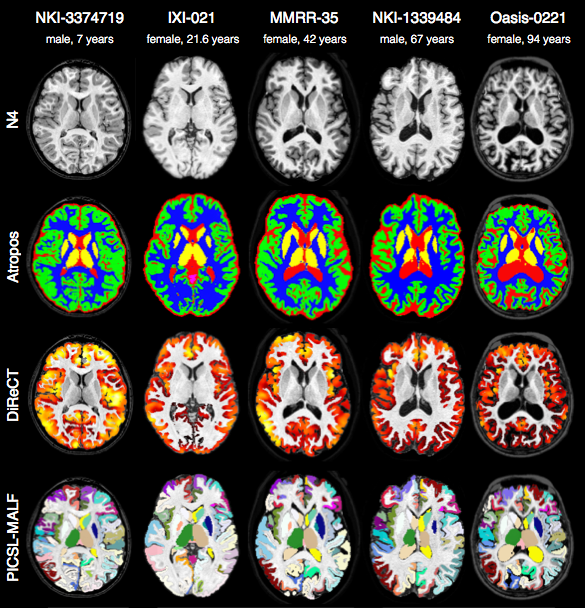
\includegraphics{./evaluation/figures/components.png}

\end{frame}

\begin{frame}{The ANTs structural brain mapping workflow}

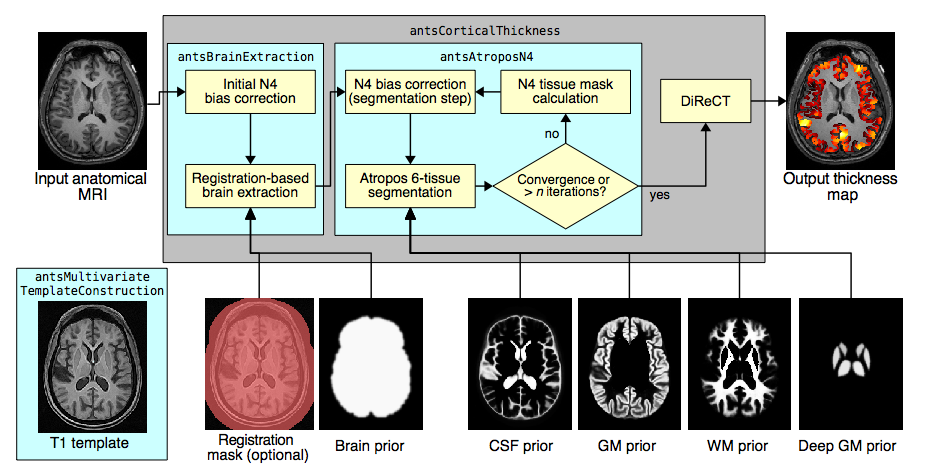
\includegraphics{./evaluation/figures/pipeline.png}

\end{frame}

\begin{frame}{Template building}

\emph{Tailor data to your specific cohort}

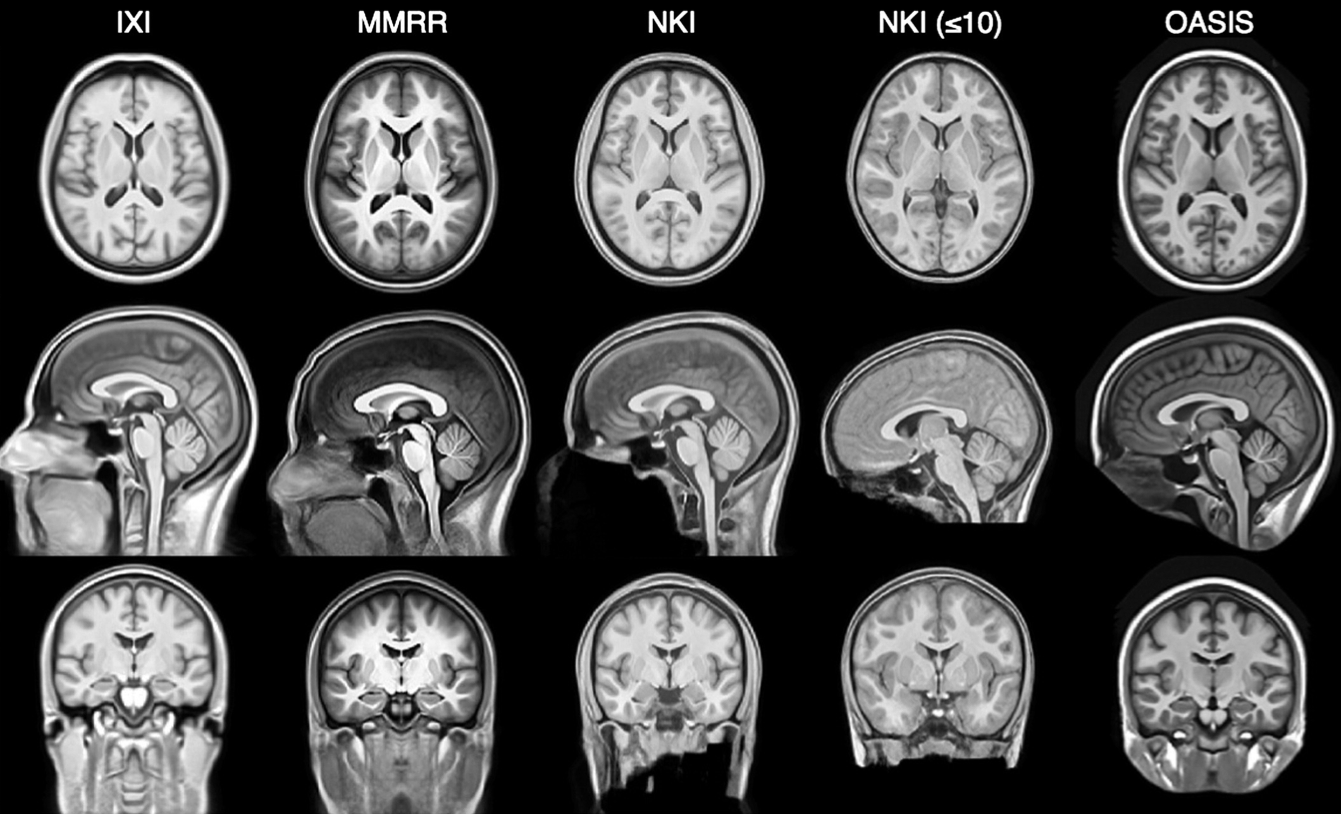
\includegraphics{./evaluation/figures/templates.png}

\end{frame}

\begin{frame}{Template priors}

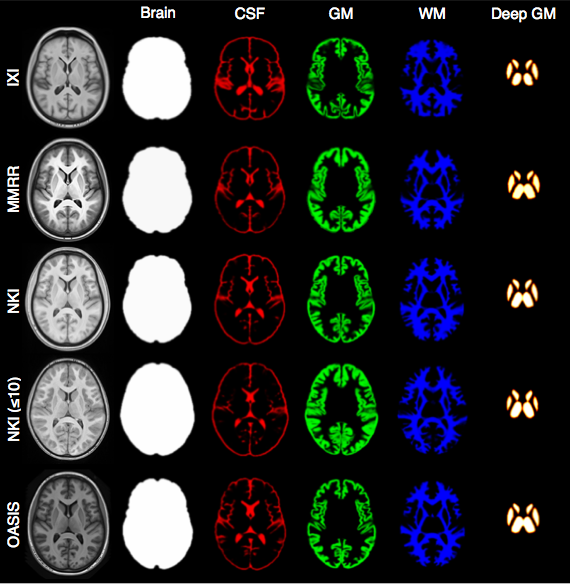
\includegraphics{./evaluation/figures/templatePriors.png}

\end{frame}

\begin{frame}{Cortical thickness maps}

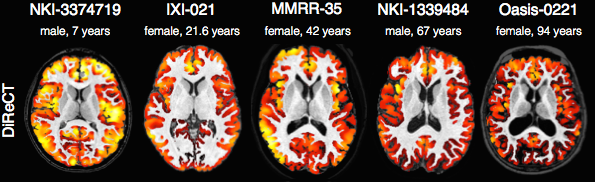
\includegraphics{./evaluation/figures/corticalThicknessEstimation.png}

In contrast to FreeSurfer which warps coupled surface meshes to segment
the gray matter, \emph{ANTs} diffeomorphically registers the white
matter to the combined gray/white matters while simultaneously
estimating thickness.

\end{frame}

\begin{frame}

\emph{But without ground truth, how does one evaluate the pipeline?}

\end{frame}

\begin{frame}{Predict age and gender}

\(AGE \sim VOLUME + GENDER + \sum_{i=1}^{62} T(DKT_i)\)

\end{frame}

\begin{frame}{Open science principles}

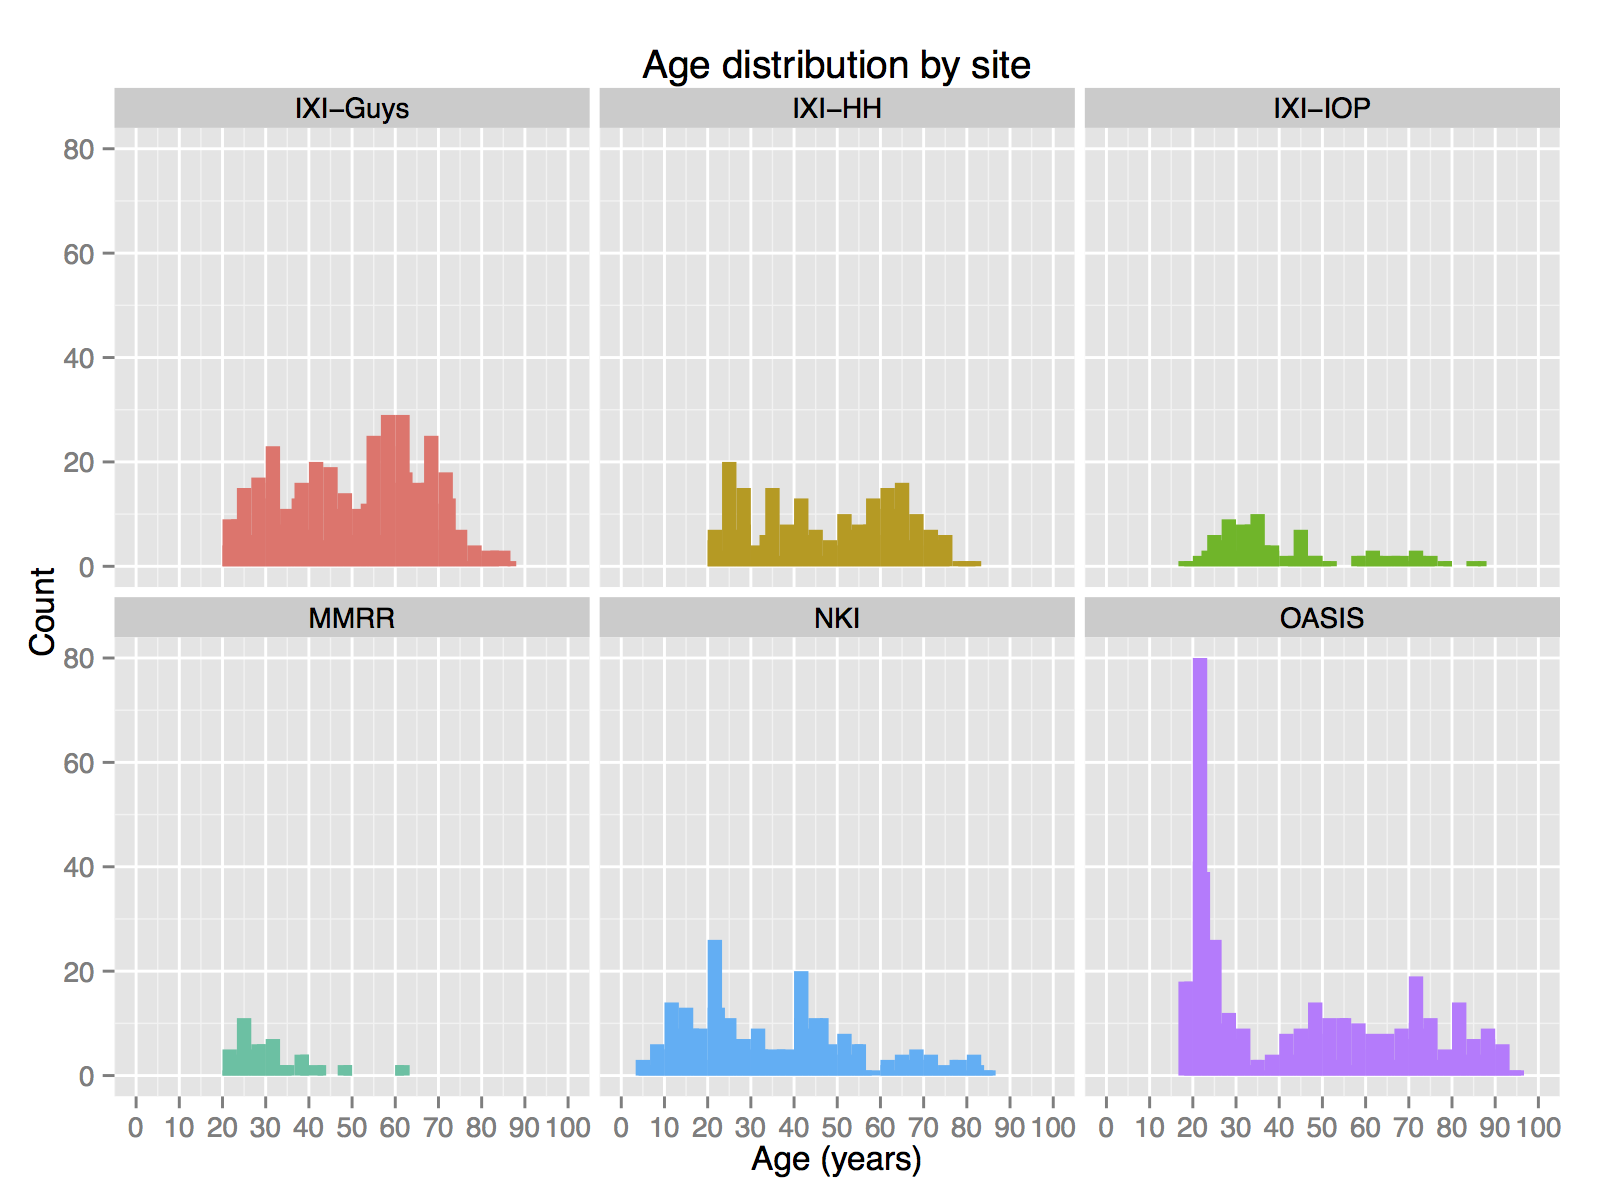
\includegraphics{./evaluation/figures/ageDistribution.png}

\end{frame}

\begin{frame}{Prediction from cortical thickness data}

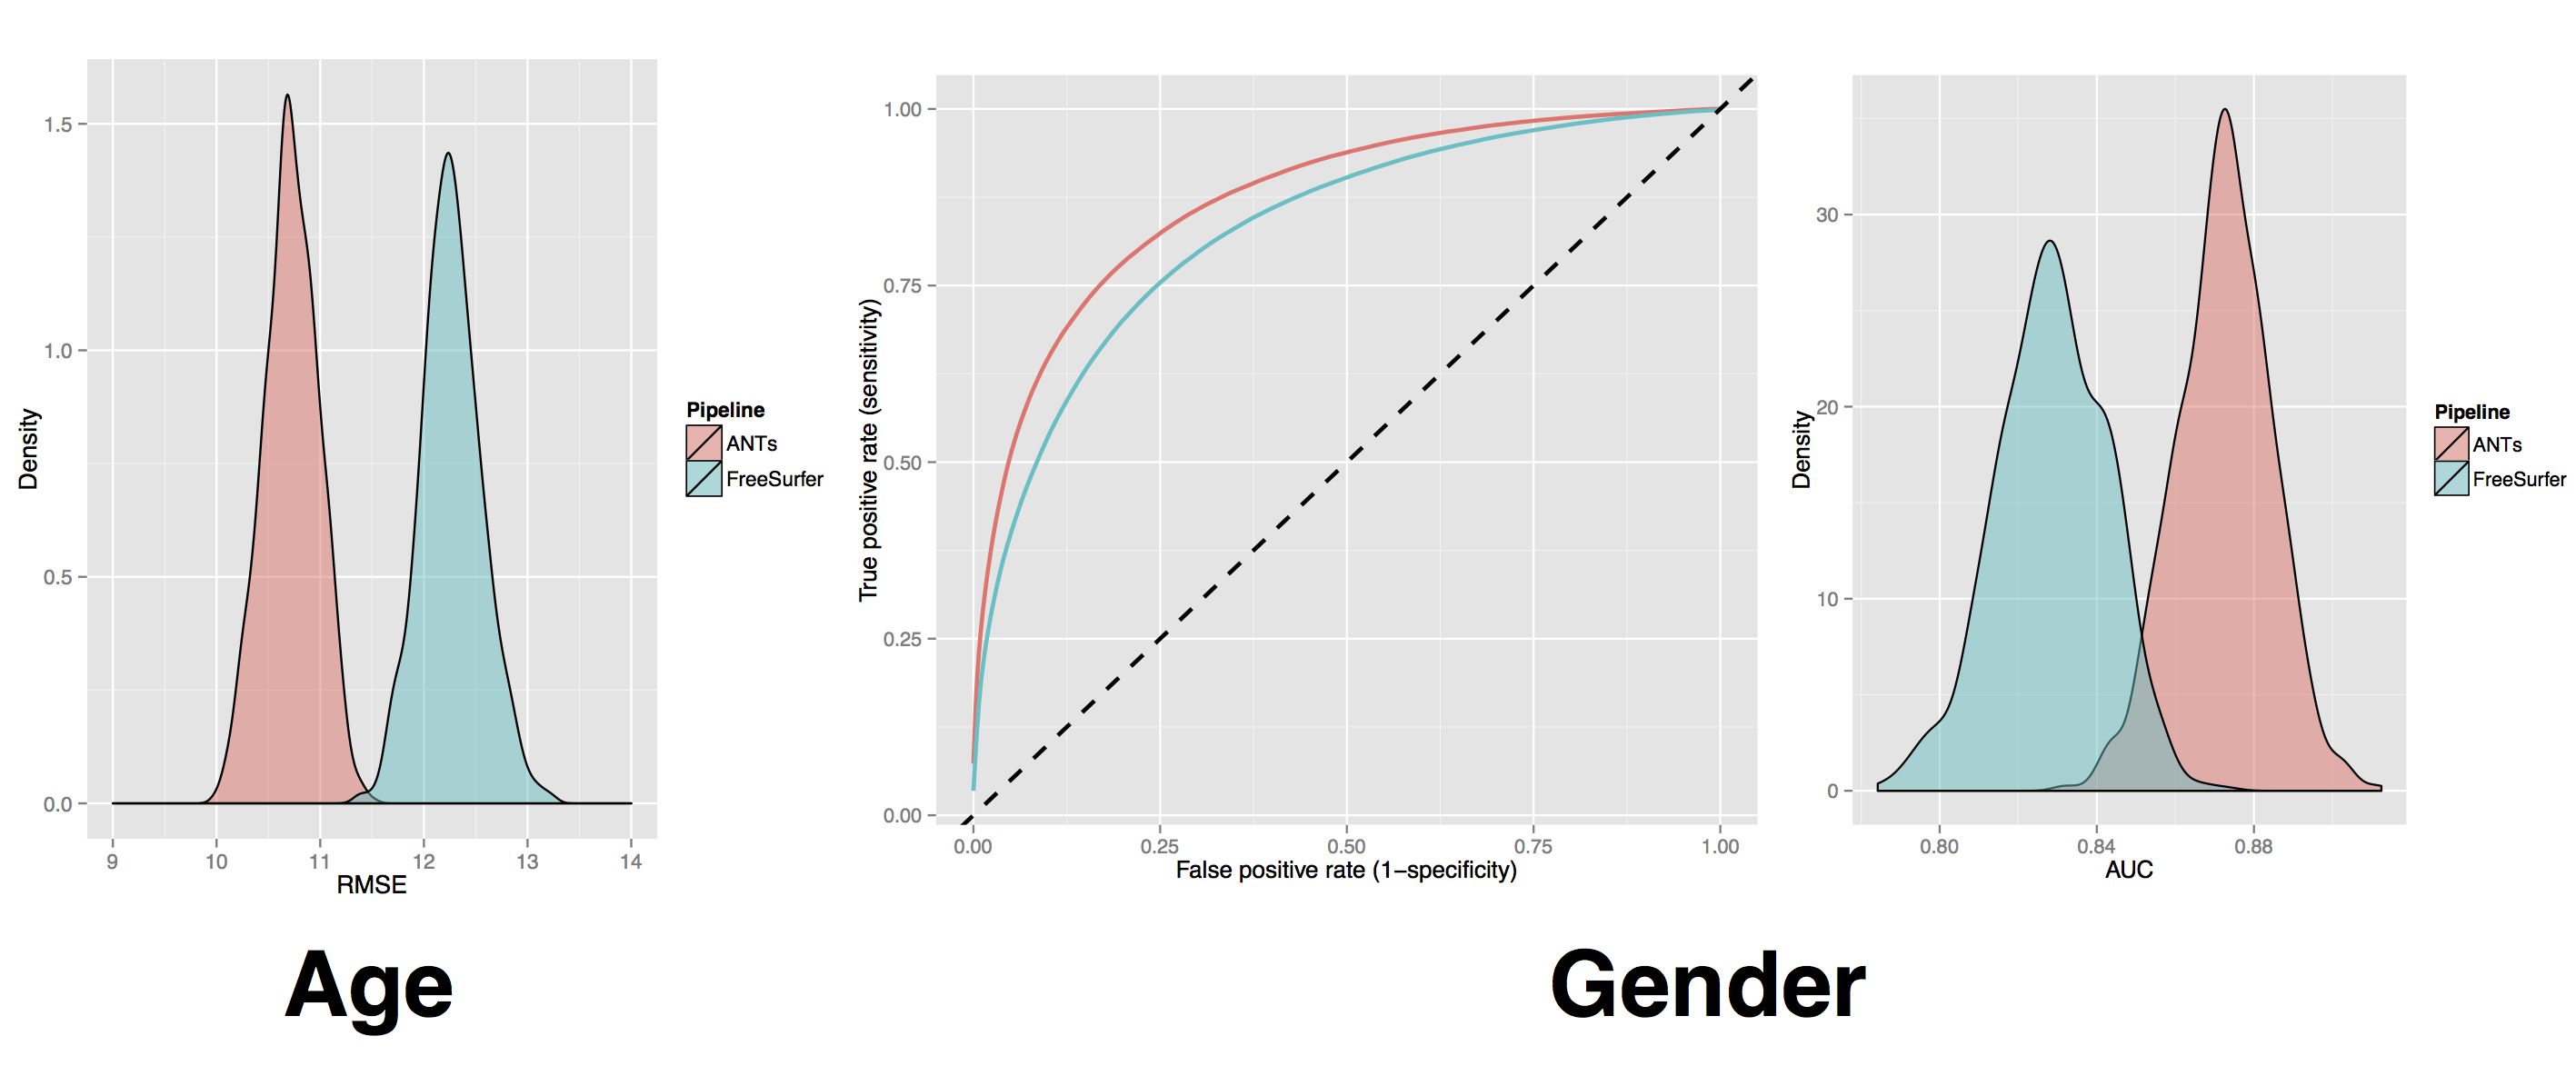
\includegraphics{./evaluation/figures/evaluation.png}

\end{frame}

\begin{frame}{Age prediction per site}

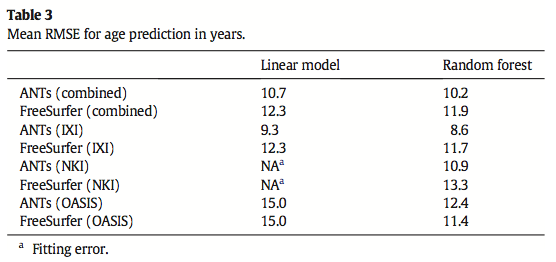
\includegraphics{./evaluation/figures/agePredictionPerSite.png}

\end{frame}

\begin{frame}{Regional importance comparison}

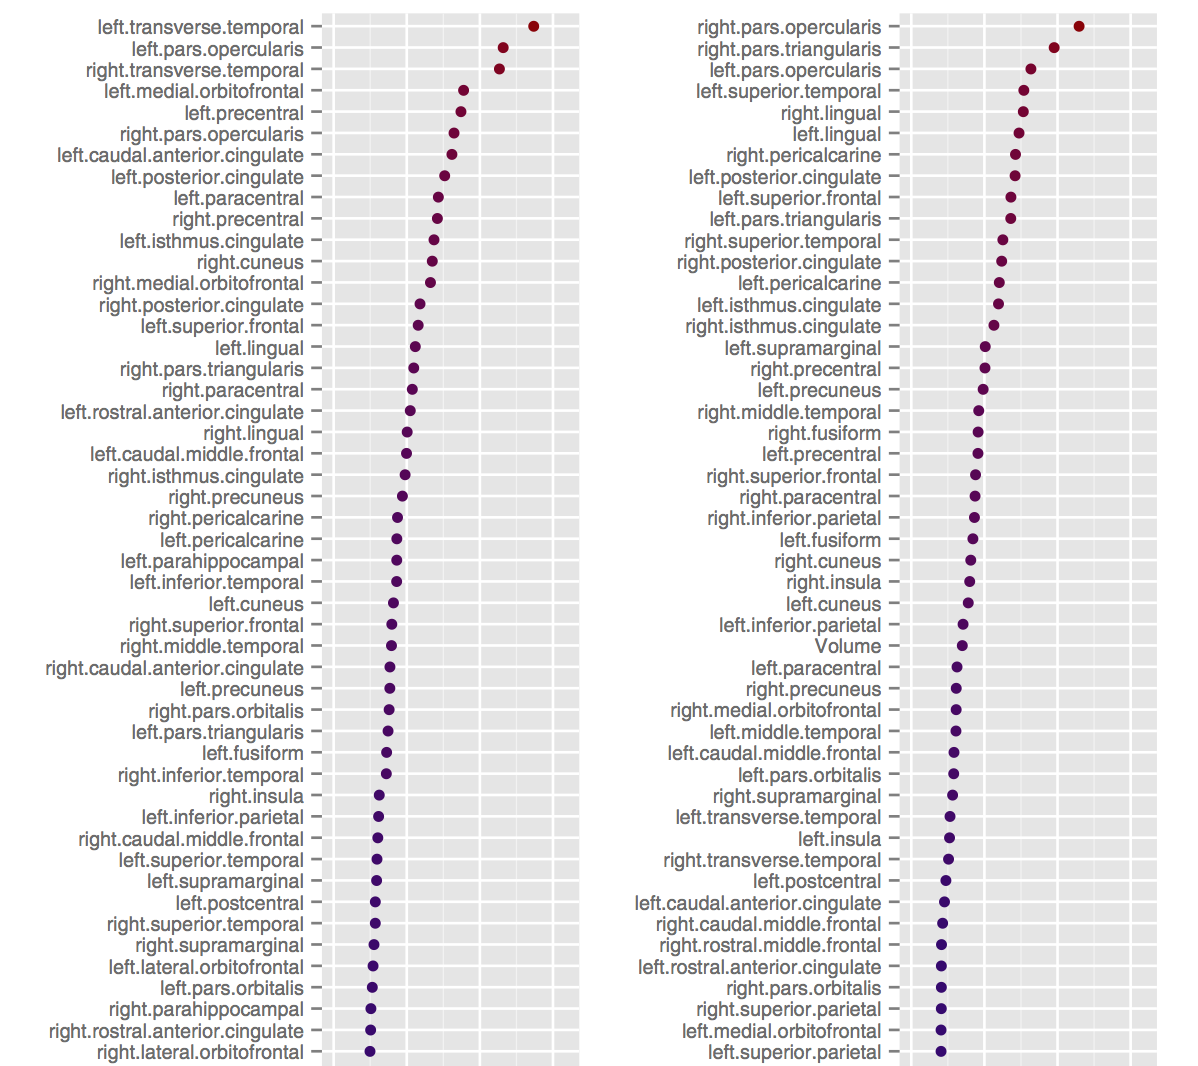
\includegraphics{./evaluation/figures/antsvfreesurfer_Importance.png}

ANTs (left) vs.~FreeSurfer (right)

\end{frame}

\begin{frame}{Regional measurements}

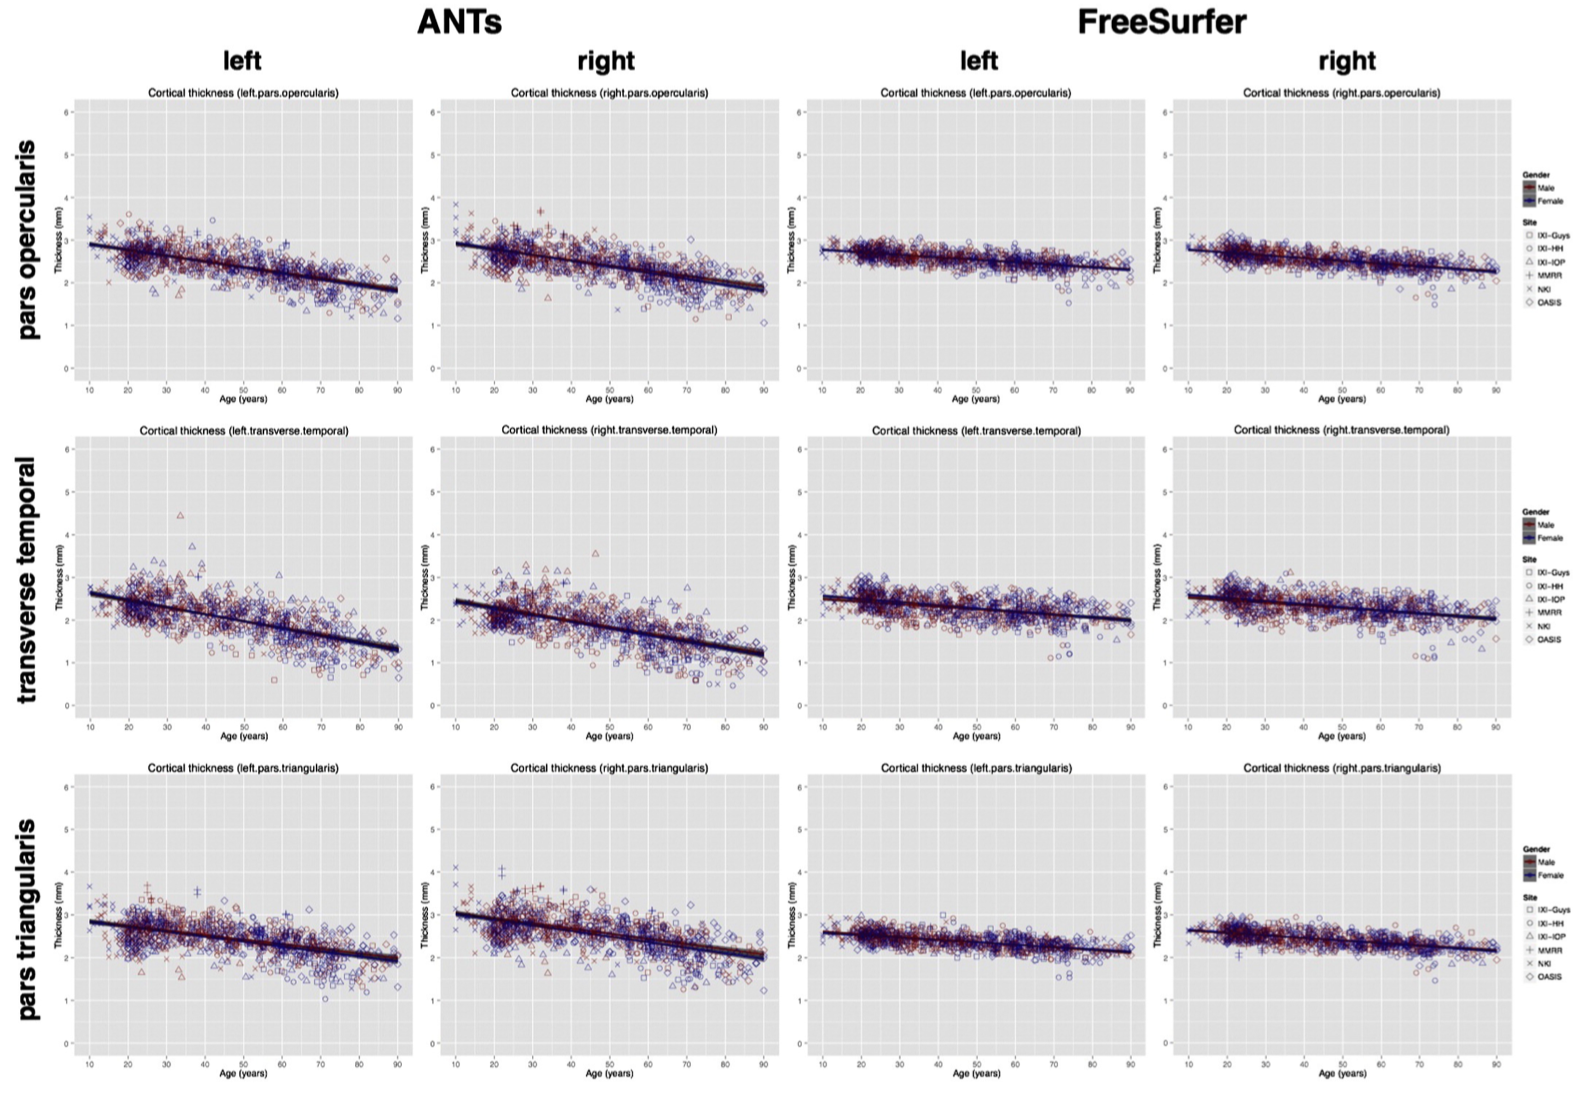
\includegraphics{./evaluation/figures/antsvfreesurfer_regionalPlots.png}

\end{frame}

\section{But, wait, there's more!}\label{but-wait-theres-more}

\begin{frame}{ANTs tools are multivariate}

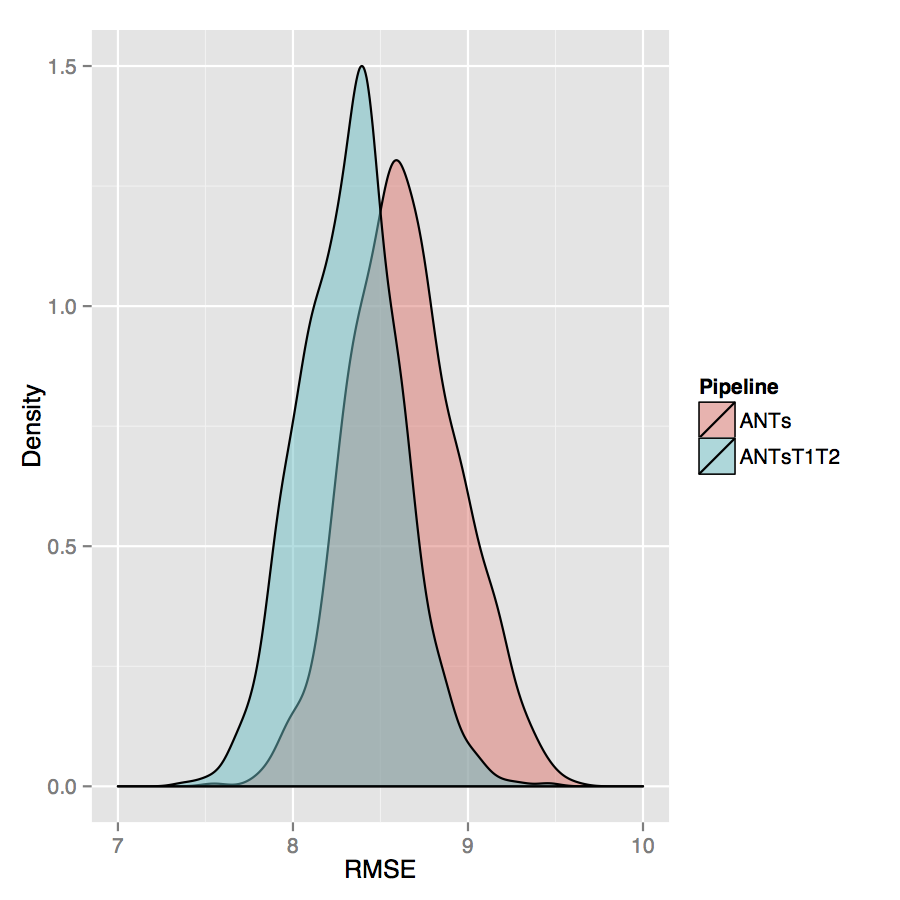
\includegraphics{./evaluation/figures/rfRmse05ANTsT1T2.png}

\end{frame}

\begin{frame}{Arno-thick-in-the-head (ATITH)}

\emph{What if we made a crude estimate of the cortical thickness?}

\[thickness_{ROI} = \frac{volume_{ROI}}{area_{ROI}}\]

\end{frame}

\begin{frame}{Prediction from cortical thickness data}

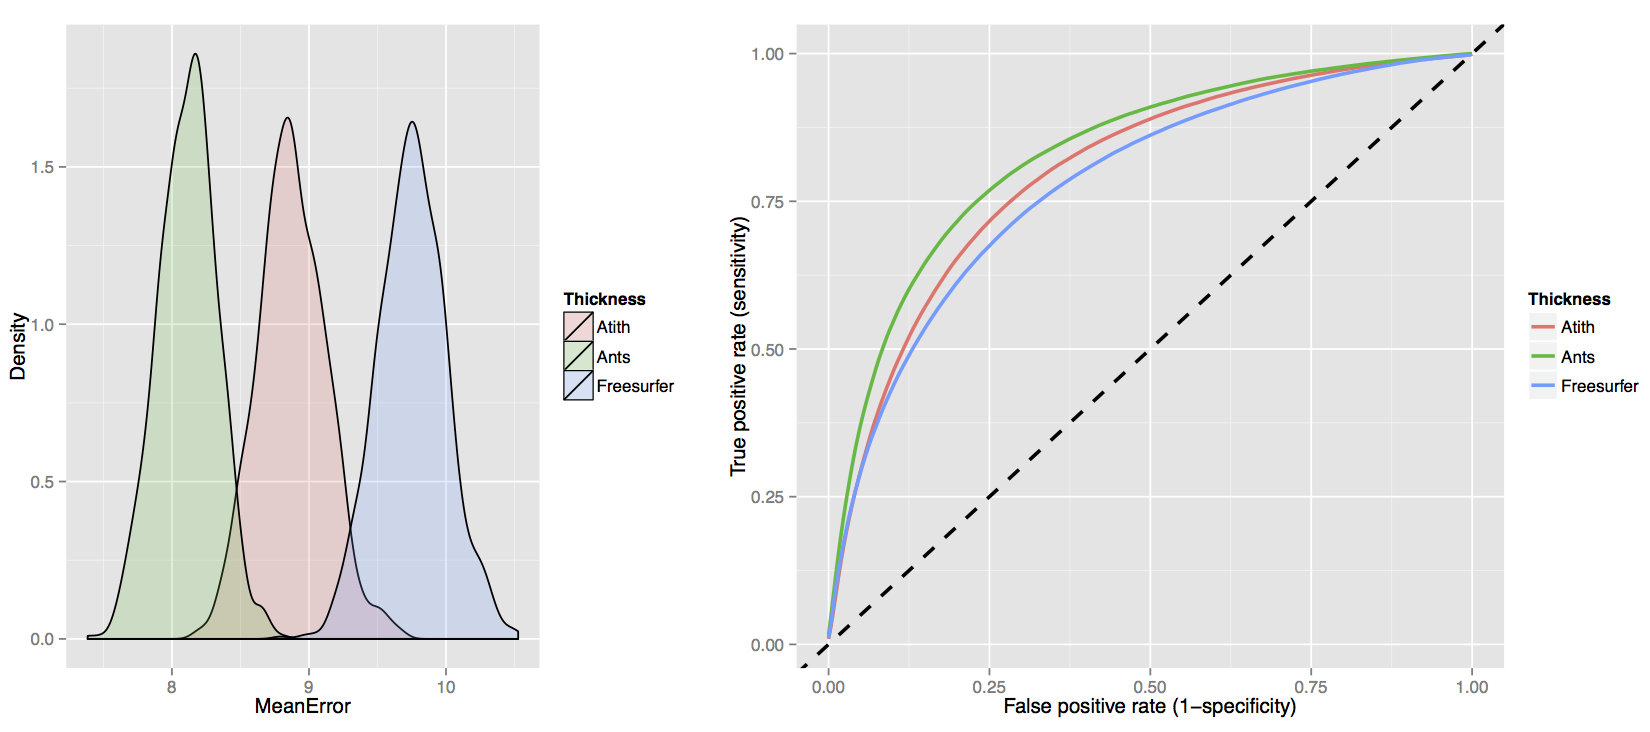
\includegraphics{./evaluation/figures/atith.png}

\end{frame}

\begin{frame}{Longitudinal processing}

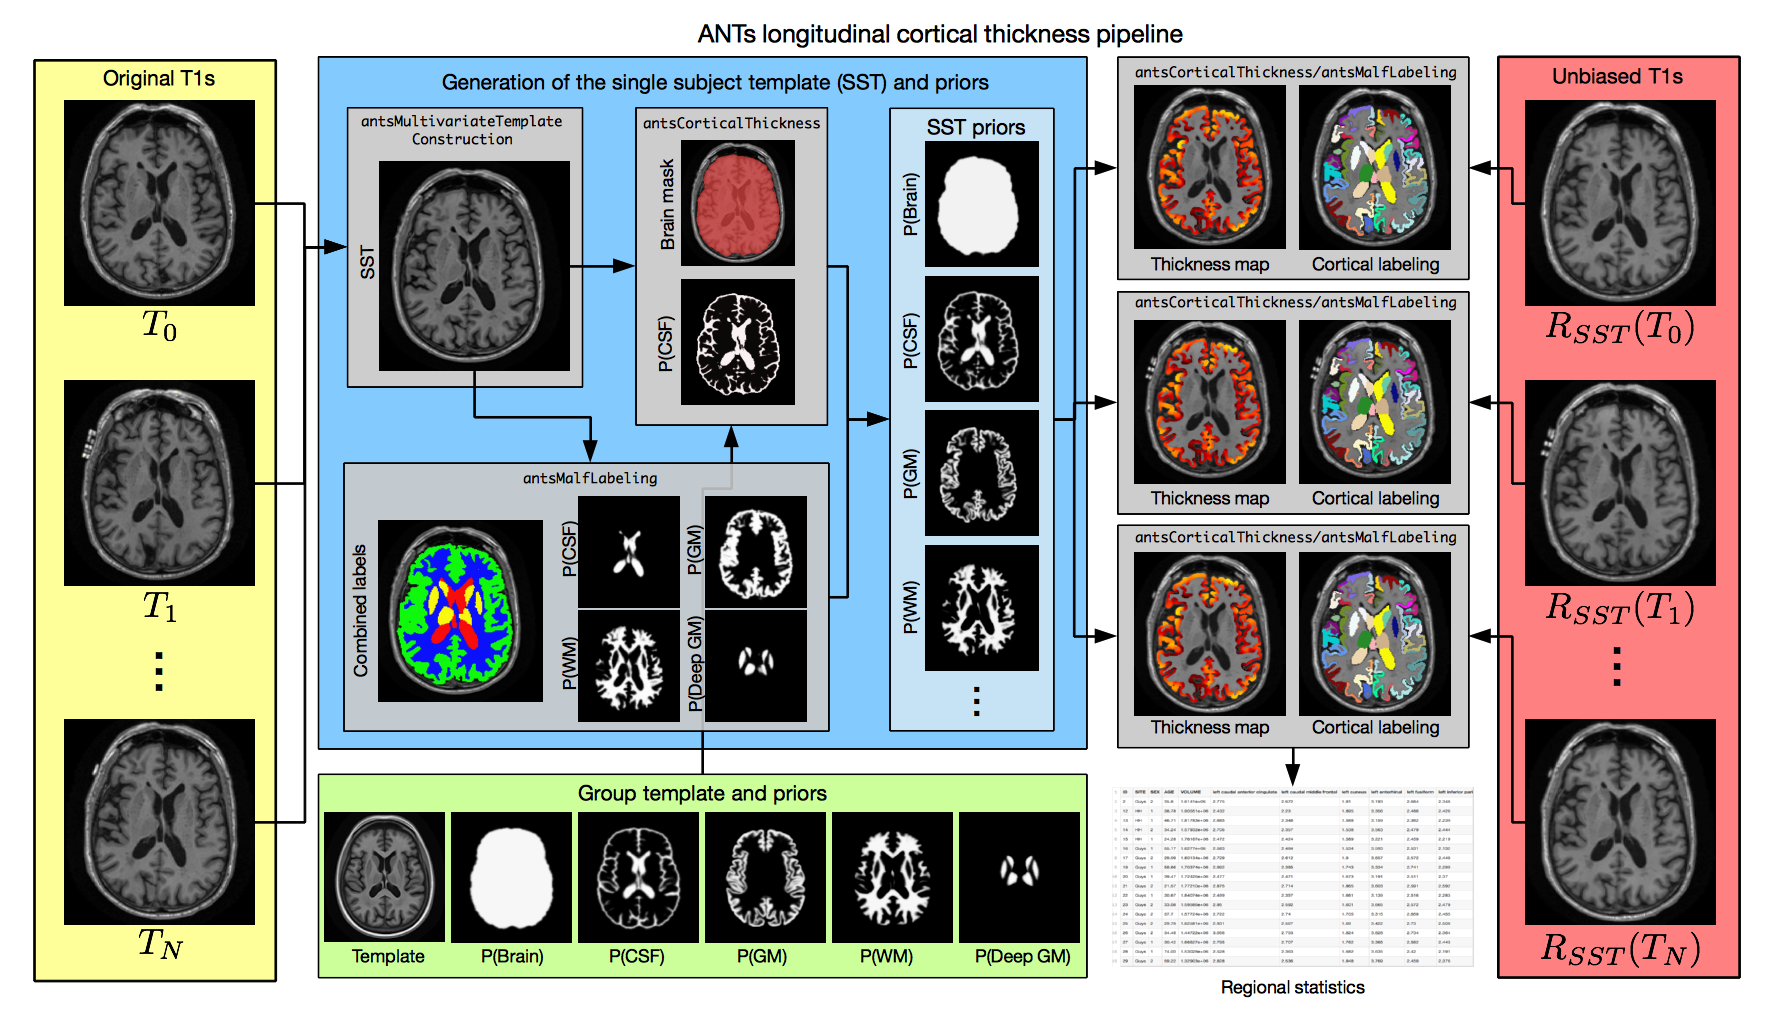
\includegraphics{./longitudinal/figures/longitudinalPipeline.png}

\end{frame}

\section{But the best part is \ldots{}}\label{but-the-best-part-is}

\begin{frame}[fragile]{it is absolutely ``free''!}

\begin{Shaded}
\begin{Highlighting}[]
\OtherTok{$\{ANTSPATH\}}\KeywordTok{/antsCorticalThickness.sh} \NormalTok{\textbackslash{}}
  \NormalTok{-a IXI/T1/IXI002-Guys-0828-T1.nii.gz \textbackslash{}}
  \NormalTok{-e IXI/template/T_template0.nii.gz \textbackslash{}}
  \NormalTok{-m IXI/template/T_template0ProbabilityMask.nii.gz \textbackslash{}}
  \NormalTok{-f IXI/template/T_template0ExtractionMask.nii.gz \textbackslash{}}
  \NormalTok{-p IXI/template/Priors/priors%d.nii.gz \textbackslash{}}
  \NormalTok{-o IXI/ANTsResults/IXI002-Guys-0828-}
\end{Highlighting}
\end{Shaded}

\end{frame}

\begin{frame}

\href{https://github.com/ntustison/KapowskiChronicles}{\textbf{Data
availability}}

\begin{itemize}
\item
  ``\emph{Hey, can I have the FreeSurfer measurements for the entorhinal
  cortex?}'' Sure, why
  not?---\href{http://www.ncbi.nlm.nih.gov/pubmed/26565394}{Hasan, et
  al., J Neuroimaging}
\item
  ``\emph{Can I have one or more of the templates that you used for your
  study?}'' Would you like the priors as well?
\end{itemize}

\end{frame}

\section{Current work and Advanced Normalization Tools in R
(ANTsR)}\label{current-work-and-advanced-normalization-tools-in-r-antsr}

\begin{frame}{Multimodal Brain Tumor Segmentation (BRATS 2013)}

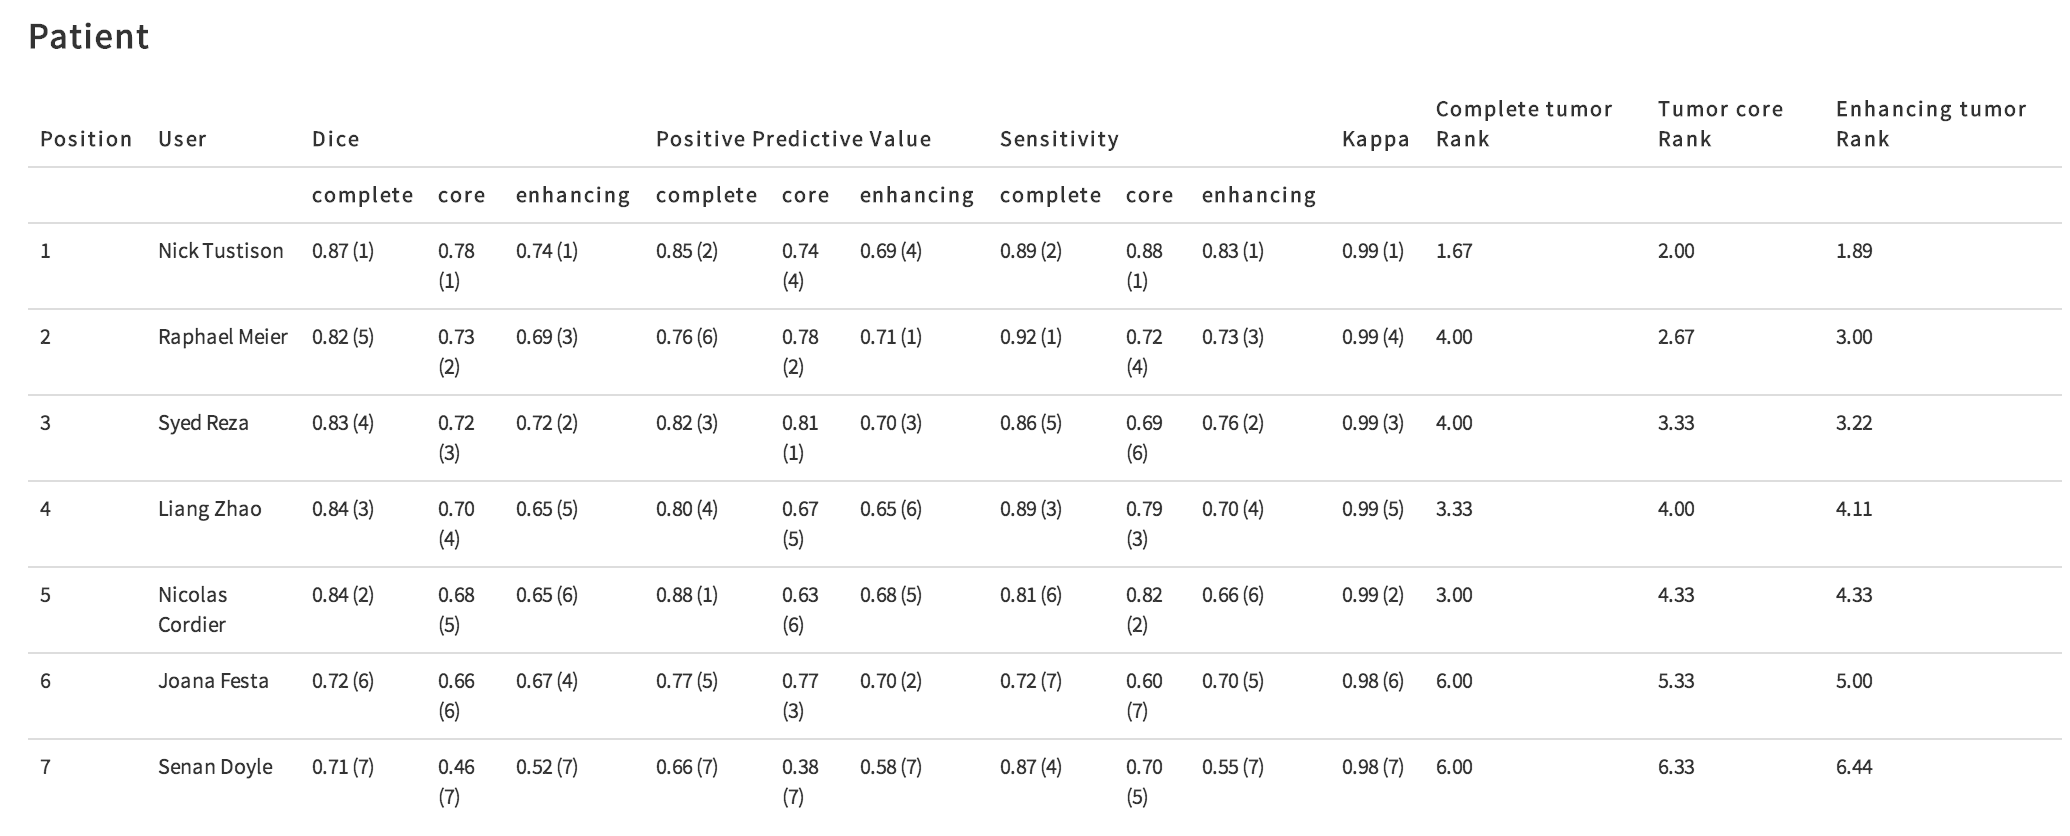
\includegraphics{./competitions/figures/brats2013results2.png}

\href{http://www.ncbi.nlm.nih.gov/pubmed/25433513}{Tustison, et al.,
Optimal symmetric multimodal templates and concatenated random forests
for supervised brain tumor segmentation (simplified) with \emph{ANTsR},
\emph{Neuroinformatics}.}

\end{frame}

\begin{frame}{White matter hyperintensities in TBI}

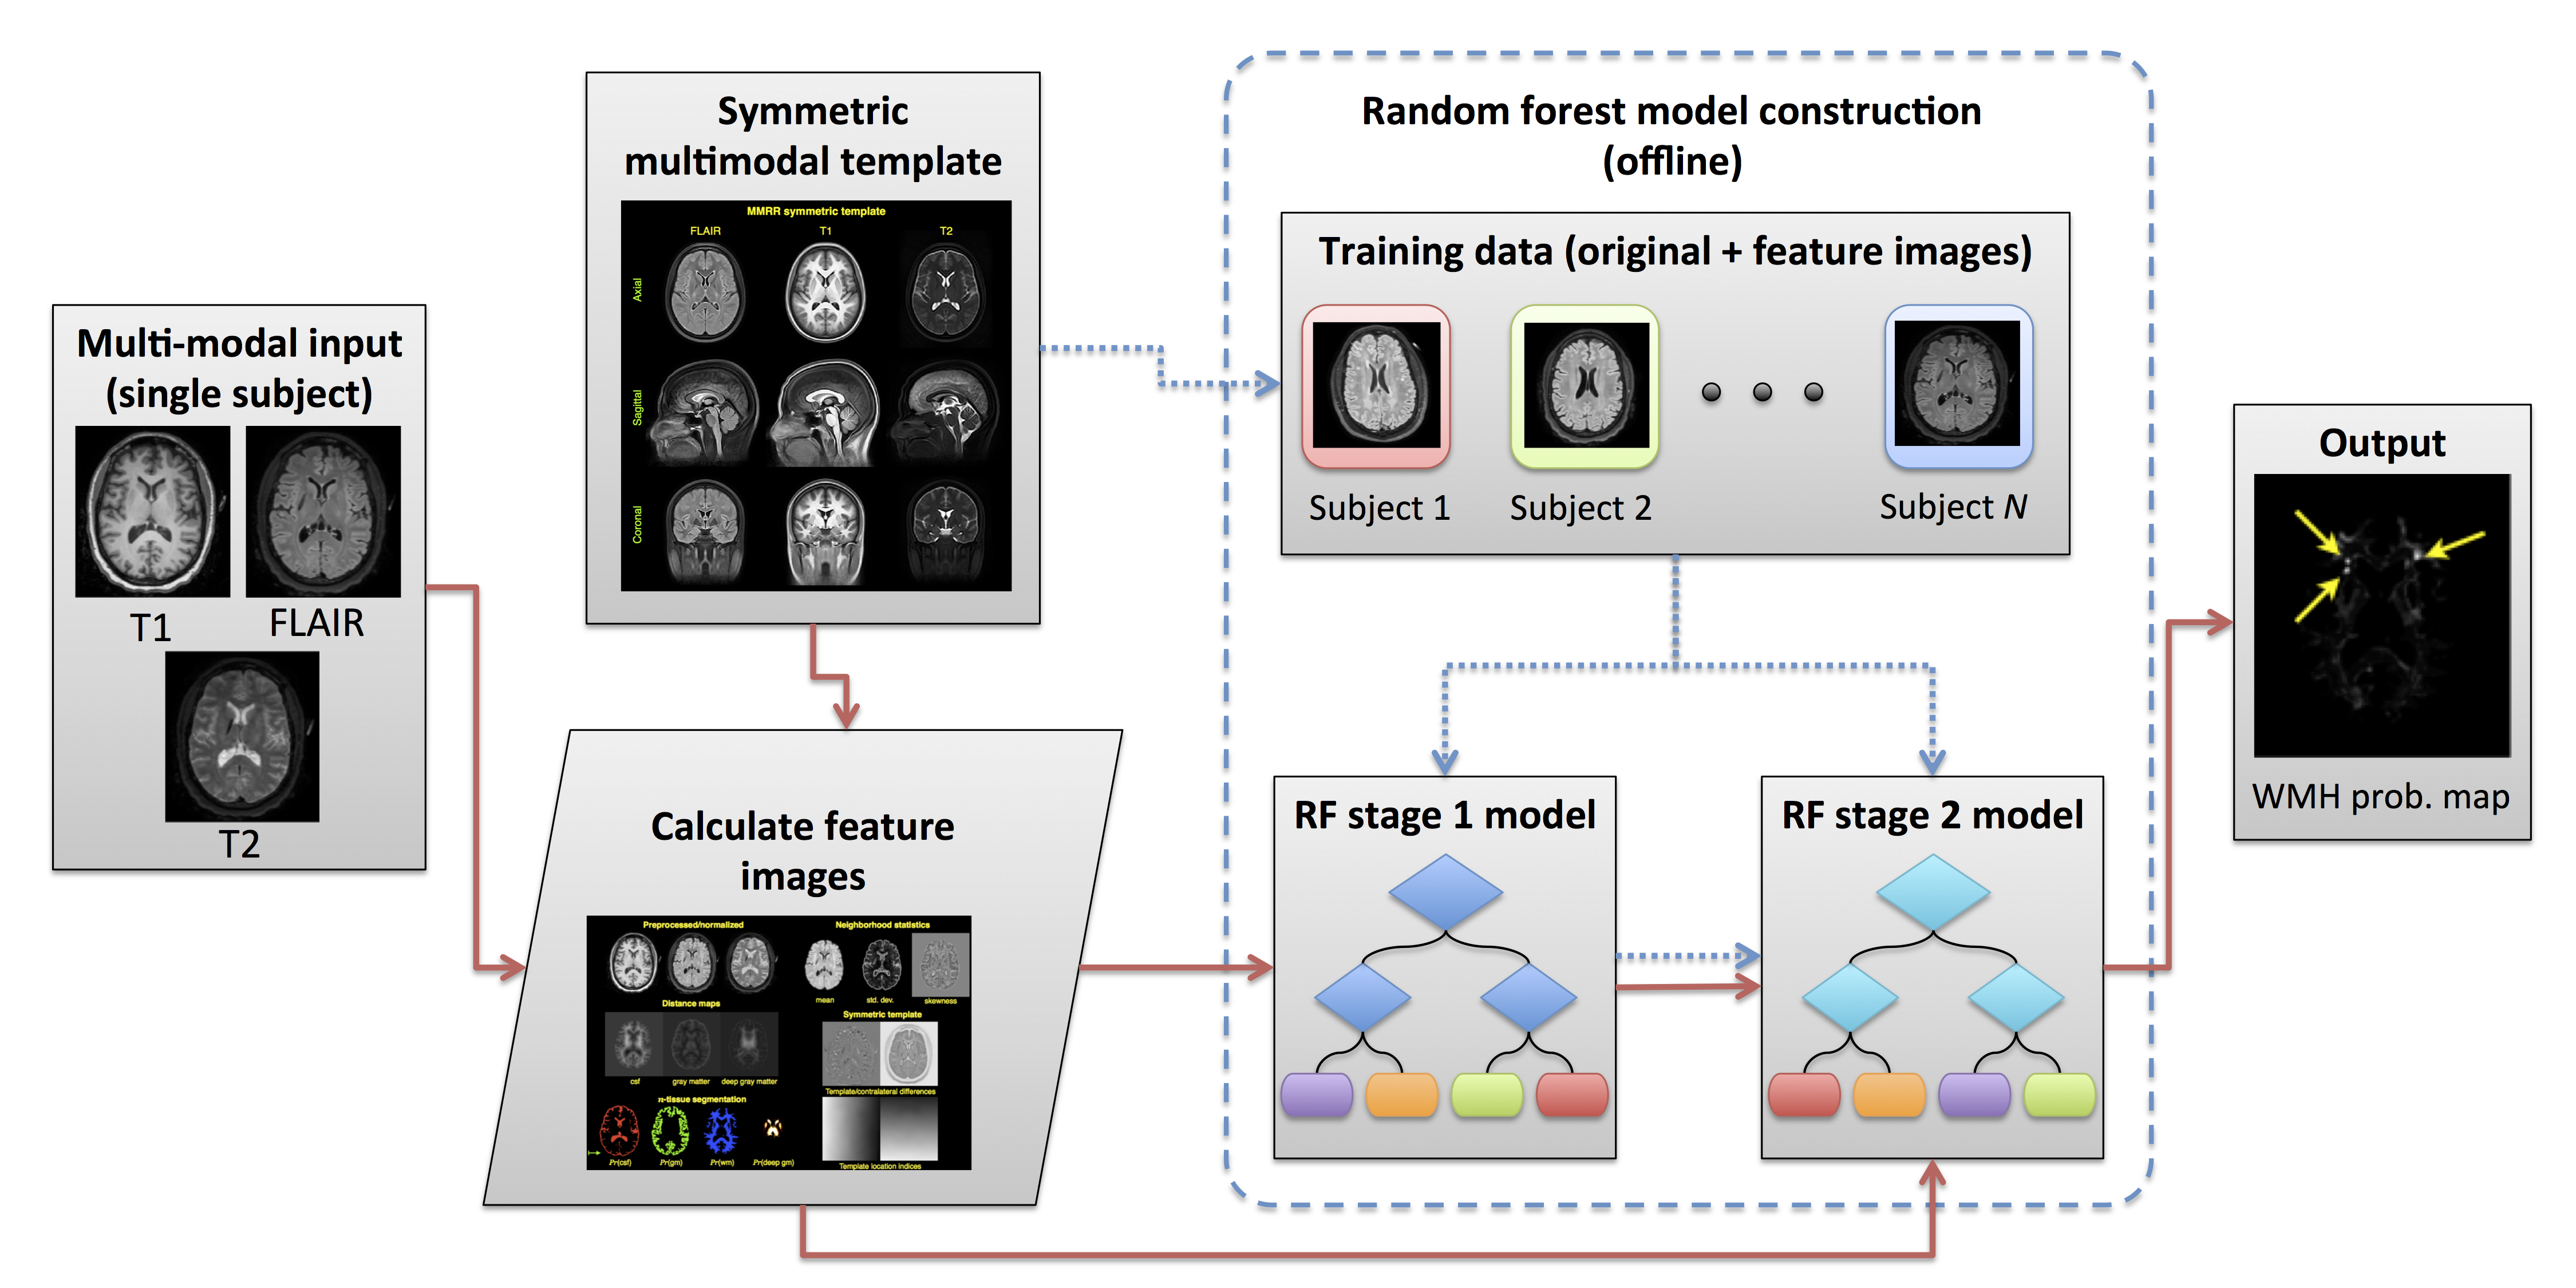
\includegraphics{./wmhs/figures/wmhPipeline.png}

\end{frame}

\begin{frame}{Social behavior and immunity dysfunction in mice}

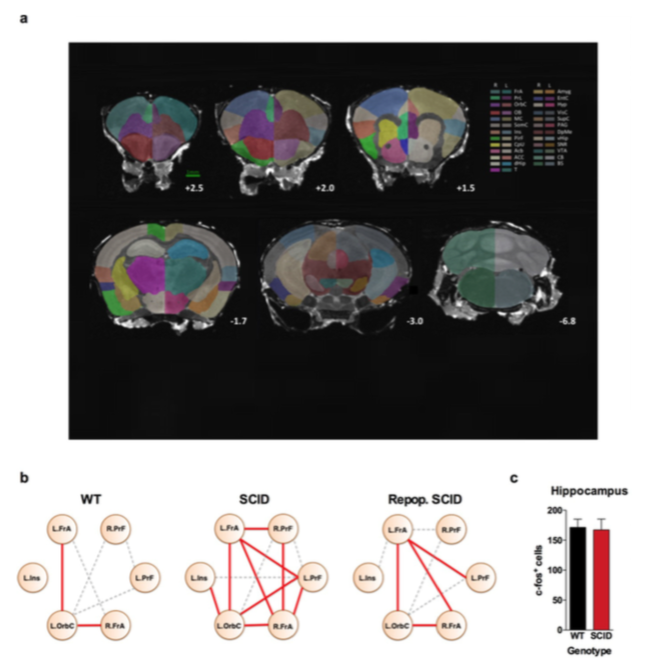
\includegraphics{./antsr/figures/filiano_rsfmri.png}

\end{frame}

\begin{frame}{Other ANTsR work}

\begin{itemize}
\item
  \href{http://www.nature.com/articles/sdata20153}{Pediatric template of
  brain perfusion}
\item
  \href{http://www.ncbi.nlm.nih.gov/pubmed/26756101}{Automated
  segmentation of chronic stroke lesions using LINDA: Lesion
  identification with neighborhood data analysis}
\item
  \href{http://www.ncbi.nlm.nih.gov/pubmed/25448483}{Eigenanatomy}
\item
  Corrective learning for segmentation refinement
\end{itemize}

\hypertarget{refs}{}

\end{frame}

\end{document}
